\documentclass[twoside]{book}

% Packages required by doxygen
\usepackage{fixltx2e}
\usepackage{calc}
\usepackage{doxygen}
\usepackage[export]{adjustbox} % also loads graphicx
\usepackage{graphicx}
\usepackage[utf8]{inputenc}
\usepackage{makeidx}
\usepackage{multicol}
\usepackage{multirow}
\PassOptionsToPackage{warn}{textcomp}
\usepackage{textcomp}
\usepackage[nointegrals]{wasysym}
\usepackage[table]{xcolor}

% Font selection
\usepackage[T1]{fontenc}
\usepackage[scaled=.90]{helvet}
\usepackage{courier}
\usepackage{amssymb}
\usepackage{sectsty}
\renewcommand{\familydefault}{\sfdefault}
\allsectionsfont{%
  \fontseries{bc}\selectfont%
  \color{darkgray}%
}
\renewcommand{\DoxyLabelFont}{%
  \fontseries{bc}\selectfont%
  \color{darkgray}%
}
\newcommand{\+}{\discretionary{\mbox{\scriptsize$\hookleftarrow$}}{}{}}

% Page & text layout
\usepackage{geometry}
\geometry{%
  a4paper,%
  top=2.5cm,%
  bottom=2.5cm,%
  left=2.5cm,%
  right=2.5cm%
}
\tolerance=750
\hfuzz=15pt
\hbadness=750
\setlength{\emergencystretch}{15pt}
\setlength{\parindent}{0cm}
\setlength{\parskip}{3ex plus 2ex minus 2ex}
\makeatletter
\renewcommand{\paragraph}{%
  \@startsection{paragraph}{4}{0ex}{-1.0ex}{1.0ex}{%
    \normalfont\normalsize\bfseries\SS@parafont%
  }%
}
\renewcommand{\subparagraph}{%
  \@startsection{subparagraph}{5}{0ex}{-1.0ex}{1.0ex}{%
    \normalfont\normalsize\bfseries\SS@subparafont%
  }%
}
\makeatother

% Headers & footers
\usepackage{fancyhdr}
\pagestyle{fancyplain}
\fancyhead[LE]{\fancyplain{}{\bfseries\thepage}}
\fancyhead[CE]{\fancyplain{}{}}
\fancyhead[RE]{\fancyplain{}{\bfseries\leftmark}}
\fancyhead[LO]{\fancyplain{}{\bfseries\rightmark}}
\fancyhead[CO]{\fancyplain{}{}}
\fancyhead[RO]{\fancyplain{}{\bfseries\thepage}}
\fancyfoot[LE]{\fancyplain{}{}}
\fancyfoot[CE]{\fancyplain{}{}}
\fancyfoot[RE]{\fancyplain{}{\bfseries\scriptsize 制作者 Doxygen }}
\fancyfoot[LO]{\fancyplain{}{\bfseries\scriptsize 制作者 Doxygen }}
\fancyfoot[CO]{\fancyplain{}{}}
\fancyfoot[RO]{\fancyplain{}{}}
\renewcommand{\footrulewidth}{0.4pt}
\renewcommand{\chaptermark}[1]{%
  \markboth{#1}{}%
}
\renewcommand{\sectionmark}[1]{%
  \markright{\thesection\ #1}%
}

% Indices & bibliography
\usepackage{natbib}
\usepackage[titles]{tocloft}
\setcounter{tocdepth}{3}
\setcounter{secnumdepth}{5}
\makeindex

% Hyperlinks (required, but should be loaded last)
\usepackage{ifpdf}
\ifpdf
  \usepackage[pdftex,pagebackref=true]{hyperref}
\else
  \usepackage[ps2pdf,pagebackref=true]{hyperref}
\fi
\hypersetup{%
  colorlinks=true,%
  linkcolor=blue,%
  citecolor=blue,%
  unicode%
}

% Custom commands
\newcommand{\clearemptydoublepage}{%
  \newpage{\pagestyle{empty}\cleardoublepage}%
}

\usepackage{caption}
\captionsetup{labelsep=space,justification=centering,font={bf},singlelinecheck=off,skip=4pt,position=top}

%===== C O N T E N T S =====

\begin{document}

% Titlepage & ToC
\hypersetup{pageanchor=false,
             bookmarksnumbered=true,
             pdfencoding=unicode
            }
\pagenumbering{alph}
\begin{titlepage}
\vspace*{7cm}
\begin{center}%
{\Large Lost Phoenix \\[1ex]\large 1.\+1 }\\
\vspace*{1cm}
{\large 制作者 Doxygen 1.8.13}\\
\end{center}
\end{titlepage}
\clearemptydoublepage
\pagenumbering{roman}
\tableofcontents
\clearemptydoublepage
\pagenumbering{arabic}
\hypersetup{pageanchor=true}

%--- Begin generated contents ---
\chapter{命名空间索引}
\section{命名空间列表}
这里列出了所有命名空间定义,附带简要说明\+:\begin{DoxyCompactList}
\item\contentsline{section}{\hyperlink{namespaceege}{ege} }{\pageref{namespaceege}}{}
\item\contentsline{section}{\hyperlink{namespace_settings}{Settings} }{\pageref{namespace_settings}}{}
\end{DoxyCompactList}

\chapter{继承关系索引}
\section{类继承关系}
此继承关系列表按字典顺序粗略的排序\+: \begin{DoxyCompactList}
\item \contentsline{section}{Settings\+:\+:Anime\+Textures}{\pageref{struct_settings_1_1_anime_textures}}{}
\item \contentsline{section}{basic\+\_\+vector2D$<$ \+\_\+\+Ty $>$}{\pageref{structbasic__vector2_d}}{}
\item \contentsline{section}{basic\+\_\+vector2D$<$ double $>$}{\pageref{structbasic__vector2_d}}{}
\item \contentsline{section}{Settings\+:\+:Bg\+Textures}{\pageref{struct_settings_1_1_bg_textures}}{}
\item \contentsline{section}{Settings\+:\+:Bullet}{\pageref{struct_settings_1_1_bullet}}{}
\item ege\+Control\+Base\begin{DoxyCompactList}
\item \contentsline{section}{Action}{\pageref{class_action}}{}
\begin{DoxyCompactList}
\item \contentsline{section}{Action\+\_\+\+Plane\+\_\+\+Explode}{\pageref{class_action___plane___explode}}{}
\end{DoxyCompactList}
\end{DoxyCompactList}
\item \contentsline{section}{Entity}{\pageref{class_entity}}{}
\begin{DoxyCompactList}
\item \contentsline{section}{Bullet}{\pageref{class_bullet}}{}
\begin{DoxyCompactList}
\item \contentsline{section}{Bullet\+\_\+\+Enemy\+\_\+\+Auto\+Target}{\pageref{class_bullet___enemy___auto_target}}{}
\item \contentsline{section}{Bullet\+\_\+\+Enemy\+\_\+\+Junior}{\pageref{class_bullet___enemy___junior}}{}
\item \contentsline{section}{Bullet\+\_\+\+Player}{\pageref{class_bullet___player}}{}
\end{DoxyCompactList}
\item \contentsline{section}{Plane}{\pageref{class_plane}}{}
\begin{DoxyCompactList}
\item \contentsline{section}{Plane\+\_\+\+Enemy\+\_\+\+Auto\+Target}{\pageref{class_plane___enemy___auto_target}}{}
\item \contentsline{section}{Plane\+\_\+\+Enemy\+\_\+\+Junior}{\pageref{class_plane___enemy___junior}}{}
\item \contentsline{section}{Plane\+\_\+\+Player}{\pageref{class_plane___player}}{}
\end{DoxyCompactList}
\end{DoxyCompactList}
\item \contentsline{section}{Settings\+:\+:General}{\pageref{struct_settings_1_1_general}}{}
\item \contentsline{section}{Input\+Controller}{\pageref{class_input_controller}}{}
\item \contentsline{section}{Settings\+:\+:Plane}{\pageref{struct_settings_1_1_plane}}{}
\item \contentsline{section}{Resources\+Loader}{\pageref{class_resources_loader}}{}
\item \contentsline{section}{Texture}{\pageref{struct_texture}}{}
\item \contentsline{section}{Settings\+:\+:Texture\+Info}{\pageref{struct_settings_1_1_texture_info}}{}
\item \contentsline{section}{World}{\pageref{class_world}}{}
\end{DoxyCompactList}

\chapter{类索引}
\section{类列表}
这里列出了所有类、结构、联合以及接口定义等,并附带简要说明\+:\begin{DoxyCompactList}
\item\contentsline{section}{\hyperlink{class_action}{Action} }{\pageref{class_action}}{}
\item\contentsline{section}{\hyperlink{class_action___plane___explode}{Action\+\_\+\+Plane\+\_\+\+Explode} }{\pageref{class_action___plane___explode}}{}
\item\contentsline{section}{\hyperlink{struct_settings_1_1_anime_textures}{Settings\+::\+Anime\+Textures} \\*所有动画、\hyperlink{class_action}{Action}相关材质设置。 }{\pageref{struct_settings_1_1_anime_textures}}{}
\item\contentsline{section}{\hyperlink{structbasic__vector2_d}{basic\+\_\+vector2\+D$<$ \+\_\+\+Ty $>$} \\*数学二维向量模板类。 }{\pageref{structbasic__vector2_d}}{}
\item\contentsline{section}{\hyperlink{struct_settings_1_1_bg_textures}{Settings\+::\+Bg\+Textures} \\*所有游戏背景材质设置。 }{\pageref{struct_settings_1_1_bg_textures}}{}
\item\contentsline{section}{\hyperlink{struct_settings_1_1_bullet}{Settings\+::\+Bullet} \\*子弹的设置基类。 }{\pageref{struct_settings_1_1_bullet}}{}
\item\contentsline{section}{\hyperlink{class_bullet}{Bullet} }{\pageref{class_bullet}}{}
\item\contentsline{section}{\hyperlink{class_bullet___enemy___auto_target}{Bullet\+\_\+\+Enemy\+\_\+\+Auto\+Target} }{\pageref{class_bullet___enemy___auto_target}}{}
\item\contentsline{section}{\hyperlink{class_bullet___enemy___junior}{Bullet\+\_\+\+Enemy\+\_\+\+Junior} }{\pageref{class_bullet___enemy___junior}}{}
\item\contentsline{section}{\hyperlink{class_bullet___player}{Bullet\+\_\+\+Player} }{\pageref{class_bullet___player}}{}
\item\contentsline{section}{\hyperlink{class_entity}{Entity} \\*游戏中所有实体的总基类。 }{\pageref{class_entity}}{}
\item\contentsline{section}{\hyperlink{struct_settings_1_1_general}{Settings\+::\+General} \\*游戏全局设置,主要包含\+U\+I与相关时间设置。 }{\pageref{struct_settings_1_1_general}}{}
\item\contentsline{section}{\hyperlink{class_input_controller}{Input\+Controller} \\*处理键盘输入的控制器类。 }{\pageref{class_input_controller}}{}
\item\contentsline{section}{\hyperlink{class_plane}{Plane} }{\pageref{class_plane}}{}
\item\contentsline{section}{\hyperlink{struct_settings_1_1_plane}{Settings\+::\+Plane} \\*飞机的设置基类。 }{\pageref{struct_settings_1_1_plane}}{}
\item\contentsline{section}{\hyperlink{class_plane___enemy___auto_target}{Plane\+\_\+\+Enemy\+\_\+\+Auto\+Target} }{\pageref{class_plane___enemy___auto_target}}{}
\item\contentsline{section}{\hyperlink{class_plane___enemy___junior}{Plane\+\_\+\+Enemy\+\_\+\+Junior} }{\pageref{class_plane___enemy___junior}}{}
\item\contentsline{section}{\hyperlink{class_plane___player}{Plane\+\_\+\+Player} }{\pageref{class_plane___player}}{}
\item\contentsline{section}{\hyperlink{class_resources_loader}{Resources\+Loader} }{\pageref{class_resources_loader}}{}
\item\contentsline{section}{\hyperlink{struct_texture}{Texture} \\*表征图像材质的结构体。 }{\pageref{struct_texture}}{}
\item\contentsline{section}{\hyperlink{struct_settings_1_1_texture_info}{Settings\+::\+Texture\+Info} }{\pageref{struct_settings_1_1_texture_info}}{}
\item\contentsline{section}{\hyperlink{class_world}{World} \\*承载整个游戏运行逻辑的总类。有一个extern声明的实例。 }{\pageref{class_world}}{}
\end{DoxyCompactList}

\chapter{文件索引}
\section{文件列表}
这里列出了所有文件,并附带简要说明\+:\begin{DoxyCompactList}
\item\contentsline{section}{D\+:/叶志浩文件夹/\+Vigilans的文档/\+Programming/\+Visual Studio/\+Projects/\+Grade 1 Summer Vacation/\+Lost Phoenix/\+Lost Phoenix/include/\hyperlink{_actions_8h}{Actions.\+h} }{\pageref{_actions_8h}}{}
\item\contentsline{section}{D\+:/叶志浩文件夹/\+Vigilans的文档/\+Programming/\+Visual Studio/\+Projects/\+Grade 1 Summer Vacation/\+Lost Phoenix/\+Lost Phoenix/include/\hyperlink{_enemy___auto_target_8h}{Enemy\+\_\+\+Auto\+Target.\+h} }{\pageref{_enemy___auto_target_8h}}{}
\item\contentsline{section}{D\+:/叶志浩文件夹/\+Vigilans的文档/\+Programming/\+Visual Studio/\+Projects/\+Grade 1 Summer Vacation/\+Lost Phoenix/\+Lost Phoenix/include/\hyperlink{_enemy___cruiser_8h}{Enemy\+\_\+\+Cruiser.\+h} }{\pageref{_enemy___cruiser_8h}}{}
\item\contentsline{section}{D\+:/叶志浩文件夹/\+Vigilans的文档/\+Programming/\+Visual Studio/\+Projects/\+Grade 1 Summer Vacation/\+Lost Phoenix/\+Lost Phoenix/include/\hyperlink{_enemy___junior_8h}{Enemy\+\_\+\+Junior.\+h} }{\pageref{_enemy___junior_8h}}{}
\item\contentsline{section}{D\+:/叶志浩文件夹/\+Vigilans的文档/\+Programming/\+Visual Studio/\+Projects/\+Grade 1 Summer Vacation/\+Lost Phoenix/\+Lost Phoenix/include/\hyperlink{_entity_8h}{Entity.\+h} }{\pageref{_entity_8h}}{}
\item\contentsline{section}{D\+:/叶志浩文件夹/\+Vigilans的文档/\+Programming/\+Visual Studio/\+Projects/\+Grade 1 Summer Vacation/\+Lost Phoenix/\+Lost Phoenix/include/\hyperlink{_input_controller_8h}{Input\+Controller.\+h} }{\pageref{_input_controller_8h}}{}
\item\contentsline{section}{D\+:/叶志浩文件夹/\+Vigilans的文档/\+Programming/\+Visual Studio/\+Projects/\+Grade 1 Summer Vacation/\+Lost Phoenix/\+Lost Phoenix/include/\hyperlink{_plane_01-_01_bullet_8h}{Plane -\/ Bullet.\+h} }{\pageref{_plane_01-_01_bullet_8h}}{}
\item\contentsline{section}{D\+:/叶志浩文件夹/\+Vigilans的文档/\+Programming/\+Visual Studio/\+Projects/\+Grade 1 Summer Vacation/\+Lost Phoenix/\+Lost Phoenix/include/\hyperlink{_player_8h}{Player.\+h} }{\pageref{_player_8h}}{}
\item\contentsline{section}{D\+:/叶志浩文件夹/\+Vigilans的文档/\+Programming/\+Visual Studio/\+Projects/\+Grade 1 Summer Vacation/\+Lost Phoenix/\+Lost Phoenix/include/\hyperlink{_resources_8h}{Resources.\+h} }{\pageref{_resources_8h}}{}
\item\contentsline{section}{D\+:/叶志浩文件夹/\+Vigilans的文档/\+Programming/\+Visual Studio/\+Projects/\+Grade 1 Summer Vacation/\+Lost Phoenix/\+Lost Phoenix/include/\hyperlink{_vector2_d_8hpp}{Vector2\+D.\+hpp} }{\pageref{_vector2_d_8hpp}}{}
\item\contentsline{section}{D\+:/叶志浩文件夹/\+Vigilans的文档/\+Programming/\+Visual Studio/\+Projects/\+Grade 1 Summer Vacation/\+Lost Phoenix/\+Lost Phoenix/include/\hyperlink{_world_8h}{World.\+h} }{\pageref{_world_8h}}{}
\item\contentsline{section}{D\+:/叶志浩文件夹/\+Vigilans的文档/\+Programming/\+Visual Studio/\+Projects/\+Grade 1 Summer Vacation/\+Lost Phoenix/\+Lost Phoenix/src/\hyperlink{_actions_8cpp}{Actions.\+cpp} }{\pageref{_actions_8cpp}}{}
\item\contentsline{section}{D\+:/叶志浩文件夹/\+Vigilans的文档/\+Programming/\+Visual Studio/\+Projects/\+Grade 1 Summer Vacation/\+Lost Phoenix/\+Lost Phoenix/src/\hyperlink{_enemy___auto_target_8cpp}{Enemy\+\_\+\+Auto\+Target.\+cpp} }{\pageref{_enemy___auto_target_8cpp}}{}
\item\contentsline{section}{D\+:/叶志浩文件夹/\+Vigilans的文档/\+Programming/\+Visual Studio/\+Projects/\+Grade 1 Summer Vacation/\+Lost Phoenix/\+Lost Phoenix/src/\hyperlink{_enemy___cruiser_8cpp}{Enemy\+\_\+\+Cruiser.\+cpp} }{\pageref{_enemy___cruiser_8cpp}}{}
\item\contentsline{section}{D\+:/叶志浩文件夹/\+Vigilans的文档/\+Programming/\+Visual Studio/\+Projects/\+Grade 1 Summer Vacation/\+Lost Phoenix/\+Lost Phoenix/src/\hyperlink{_enemy___junior_8cpp}{Enemy\+\_\+\+Junior.\+cpp} }{\pageref{_enemy___junior_8cpp}}{}
\item\contentsline{section}{D\+:/叶志浩文件夹/\+Vigilans的文档/\+Programming/\+Visual Studio/\+Projects/\+Grade 1 Summer Vacation/\+Lost Phoenix/\+Lost Phoenix/src/\hyperlink{_entity_8cpp}{Entity.\+cpp} }{\pageref{_entity_8cpp}}{}
\item\contentsline{section}{D\+:/叶志浩文件夹/\+Vigilans的文档/\+Programming/\+Visual Studio/\+Projects/\+Grade 1 Summer Vacation/\+Lost Phoenix/\+Lost Phoenix/src/\hyperlink{_input_controller_8cpp}{Input\+Controller.\+cpp} }{\pageref{_input_controller_8cpp}}{}
\item\contentsline{section}{D\+:/叶志浩文件夹/\+Vigilans的文档/\+Programming/\+Visual Studio/\+Projects/\+Grade 1 Summer Vacation/\+Lost Phoenix/\+Lost Phoenix/src/\hyperlink{main_8cpp}{main.\+cpp} }{\pageref{main_8cpp}}{}
\item\contentsline{section}{D\+:/叶志浩文件夹/\+Vigilans的文档/\+Programming/\+Visual Studio/\+Projects/\+Grade 1 Summer Vacation/\+Lost Phoenix/\+Lost Phoenix/src/\hyperlink{_plane_01-_01_bullet_8cpp}{Plane -\/ Bullet.\+cpp} }{\pageref{_plane_01-_01_bullet_8cpp}}{}
\item\contentsline{section}{D\+:/叶志浩文件夹/\+Vigilans的文档/\+Programming/\+Visual Studio/\+Projects/\+Grade 1 Summer Vacation/\+Lost Phoenix/\+Lost Phoenix/src/\hyperlink{_player_8cpp}{Player.\+cpp} }{\pageref{_player_8cpp}}{}
\item\contentsline{section}{D\+:/叶志浩文件夹/\+Vigilans的文档/\+Programming/\+Visual Studio/\+Projects/\+Grade 1 Summer Vacation/\+Lost Phoenix/\+Lost Phoenix/src/\hyperlink{_resources_8cpp}{Resources.\+cpp} }{\pageref{_resources_8cpp}}{}
\item\contentsline{section}{D\+:/叶志浩文件夹/\+Vigilans的文档/\+Programming/\+Visual Studio/\+Projects/\+Grade 1 Summer Vacation/\+Lost Phoenix/\+Lost Phoenix/src/\hyperlink{_resources_loader_8cpp}{Resources\+Loader.\+cpp} }{\pageref{_resources_loader_8cpp}}{}
\item\contentsline{section}{D\+:/叶志浩文件夹/\+Vigilans的文档/\+Programming/\+Visual Studio/\+Projects/\+Grade 1 Summer Vacation/\+Lost Phoenix/\+Lost Phoenix/src/\hyperlink{_resources_loader_8h}{Resources\+Loader.\+h} }{\pageref{_resources_loader_8h}}{}
\item\contentsline{section}{D\+:/叶志浩文件夹/\+Vigilans的文档/\+Programming/\+Visual Studio/\+Projects/\+Grade 1 Summer Vacation/\+Lost Phoenix/\+Lost Phoenix/src/\hyperlink{_world_8cpp}{World.\+cpp} }{\pageref{_world_8cpp}}{}
\end{DoxyCompactList}

\chapter{命名空间文档}
\hypertarget{namespaceege}{}\section{ege 命名空间参考}
\label{namespaceege}\index{ege@{ege}}
\subsection*{类型定义}
\begin{DoxyCompactItemize}
\item 
typedef I\+M\+A\+GE $\ast$ \hyperlink{namespaceege_a72e07306fee47bc08f1baf842cb681fb}{P\+I\+M\+A\+GE}
\end{DoxyCompactItemize}


\subsection{类型定义说明}
\mbox{\Hypertarget{namespaceege_a72e07306fee47bc08f1baf842cb681fb}\label{namespaceege_a72e07306fee47bc08f1baf842cb681fb}} 
\index{ege@{ege}!P\+I\+M\+A\+GE@{P\+I\+M\+A\+GE}}
\index{P\+I\+M\+A\+GE@{P\+I\+M\+A\+GE}!ege@{ege}}
\subsubsection{\texorpdfstring{P\+I\+M\+A\+GE}{PIMAGE}}
{\footnotesize\ttfamily typedef I\+M\+A\+GE$\ast$ \hyperlink{namespaceege_a72e07306fee47bc08f1baf842cb681fb}{ege\+::\+P\+I\+M\+A\+GE}}


\hypertarget{namespace_settings}{}\section{Settings 命名空间参考}
\label{namespace_settings}\index{Settings@{Settings}}


封装了游戏全局与所有实体设置的名空间。 所有获取默认设置的方法采用 {\itshape Lazy Load(延时加载)} 机制。 {\bfseries 推荐参考详细描述来获取完整信息} 。  


\subsection*{类}
\begin{DoxyCompactItemize}
\item 
struct \hyperlink{struct_settings_1_1_anime_textures}{Anime\+Textures}
\begin{DoxyCompactList}\small\item\em 所有动画、\hyperlink{class_action}{Action}相关材质设置。 \end{DoxyCompactList}\item 
struct \hyperlink{struct_settings_1_1_bg_textures}{Bg\+Textures}
\begin{DoxyCompactList}\small\item\em 所有游戏背景材质设置。 \end{DoxyCompactList}\item 
struct \hyperlink{struct_settings_1_1_bullet}{Bullet}
\begin{DoxyCompactList}\small\item\em 子弹的设置基类。 \end{DoxyCompactList}\item 
struct \hyperlink{struct_settings_1_1_general}{General}
\begin{DoxyCompactList}\small\item\em 游戏全局设置,主要包含\+U\+I与相关时间设置。 \end{DoxyCompactList}\item 
struct \hyperlink{struct_settings_1_1_plane}{Plane}
\begin{DoxyCompactList}\small\item\em 飞机的设置基类。 \end{DoxyCompactList}\item 
struct \hyperlink{struct_settings_1_1_texture_info}{Texture\+Info}
\end{DoxyCompactItemize}
\subsection*{函数}
\begin{DoxyCompactItemize}
\item 
\mbox{\Hypertarget{namespace_settings_a8d5eb32bea233e3b9ae9ce6e29b8d8bb}\label{namespace_settings_a8d5eb32bea233e3b9ae9ce6e29b8d8bb}} 
const \hyperlink{struct_settings_1_1_general}{Settings\+::\+General} \& \hyperlink{namespace_settings_a8d5eb32bea233e3b9ae9ce6e29b8d8bb}{general} ()
\begin{DoxyCompactList}\small\item\em 获取默认的全局游戏设置。采取\+Lazy Load机制。 \end{DoxyCompactList}\item 
\mbox{\Hypertarget{namespace_settings_a8bae923ac0d881b72bbec4f50730ec72}\label{namespace_settings_a8bae923ac0d881b72bbec4f50730ec72}} 
const \hyperlink{struct_settings_1_1_bg_textures}{Settings\+::\+Bg\+Textures} \& \hyperlink{namespace_settings_a8bae923ac0d881b72bbec4f50730ec72}{bg\+Textures} ()
\begin{DoxyCompactList}\small\item\em 获取默认的背景材质设置。采取\+Lazy Load机制。 \end{DoxyCompactList}\item 
\mbox{\Hypertarget{namespace_settings_ae61a4eddbf5405fae02d781d7e698413}\label{namespace_settings_ae61a4eddbf5405fae02d781d7e698413}} 
const \hyperlink{struct_settings_1_1_anime_textures}{Settings\+::\+Anime\+Textures} \& \hyperlink{namespace_settings_ae61a4eddbf5405fae02d781d7e698413}{anime\+Textures} ()
\begin{DoxyCompactList}\small\item\em 获取默认的动画材质设置。采取\+Lazy Load机制。 \end{DoxyCompactList}\item 
\mbox{\Hypertarget{namespace_settings_ab78c6dca0d1b2fc76eae348e81a3eed7}\label{namespace_settings_ab78c6dca0d1b2fc76eae348e81a3eed7}} 
const \hyperlink{struct_settings_1_1_plane}{Settings\+::\+Plane} \& \hyperlink{namespace_settings_ab78c6dca0d1b2fc76eae348e81a3eed7}{player} ()
\begin{DoxyCompactList}\small\item\em 获取默认的玩家飞机设置。采取\+Lazy Load机制。 \end{DoxyCompactList}\item 
\mbox{\Hypertarget{namespace_settings_a5d571065d327daba740814f8e90261f5}\label{namespace_settings_a5d571065d327daba740814f8e90261f5}} 
const \hyperlink{struct_settings_1_1_plane}{Settings\+::\+Plane} \& \hyperlink{namespace_settings_a5d571065d327daba740814f8e90261f5}{enemy\+\_\+junior} ()
\begin{DoxyCompactList}\small\item\em 获取默认的新兵敌机设置。采取\+Lazy Load机制。 \end{DoxyCompactList}\item 
\mbox{\Hypertarget{namespace_settings_a77e282eadc82f97cb15c2c3eef3c535b}\label{namespace_settings_a77e282eadc82f97cb15c2c3eef3c535b}} 
const \hyperlink{struct_settings_1_1_plane}{Settings\+::\+Plane} \& \hyperlink{namespace_settings_a77e282eadc82f97cb15c2c3eef3c535b}{enemy\+\_\+auto\+Target} ()
\begin{DoxyCompactList}\small\item\em 获取默认的自机狙敌机设置。采取\+Lazy Load机制。 \end{DoxyCompactList}\item 
\mbox{\Hypertarget{namespace_settings_a42e5acb521fa66b1f2311a896df95a98}\label{namespace_settings_a42e5acb521fa66b1f2311a896df95a98}} 
void {\bfseries from\+\_\+json} (const json \&j, \hyperlink{struct_settings_1_1_bullet}{Settings\+::\+Bullet} \&b)
\item 
\mbox{\Hypertarget{namespace_settings_aaba1604e449415b4bcbbb0a6e50a0ac9}\label{namespace_settings_aaba1604e449415b4bcbbb0a6e50a0ac9}} 
void {\bfseries from\+\_\+json} (const json \&j, \hyperlink{struct_settings_1_1_plane}{Settings\+::\+Plane} \&s)
\end{DoxyCompactItemize}


\subsection{详细描述}
封装了游戏全局与所有实体设置的名空间。 所有获取默认设置的方法采用 {\itshape Lazy Load(延时加载)} 机制。 {\bfseries 推荐参考详细描述来获取完整信息} 。 

这个名空间将游戏的所有设置用几个struct进行表示,以提高可读性与扩展性。

所有默认设置保存在json文件中,放置于/settings文件夹下。 相比于用一个宏头文件保存设置,使用json的可读性与结构性更强,同时在修改相关设置数据时,也不需要 {\bfseries 全部重新编译一遍} 。

运行游戏后,会陆续从json文件中读取相关设置,在堆上用一块专门的内存保存。具体机制为:
\begin{DoxyItemize}
\item 程序开始运行时,读取所有材质的索引信息到\hyperlink{struct_settings_1_1_texture_info}{Texture\+Info}的std\+::map中,为此后设置的\+Lazy Load作准备。
\item Setting名空间中提供几个获取$\ast$$\ast$默认设置引用$\ast$$\ast$的函数。此时尚未加载任何设置。
\item 当外部类调用任一\+Setting名空间的函数后,若未加载,则加载设置到堆上的一块稳定内存区域中,并返回引用。这有两个效果:
\begin{DoxyItemize}
\item 所有设置都采取了\+Lazy Load机制,这避免了在ege图形库未初始化窗口前读取材质而造成bug,同时节省内存。
\item 默认设置始终返回堆上一块稳定内存的引用,达到一处保存多处使用的效果,同时减少拷贝。
\end{DoxyItemize}
\end{DoxyItemize}





对于飞机与子弹这样的实体,设置还有另一层作用:在一个实例构造函数中使用。 实体可能有很多的属性,若全部放在构造函数中显得十分臃肿;同时,要新增一个属性,需要修改很多地方,容易出错。

因此,飞机与子弹的构造函数设计为只需要传一个 {\ttfamily 设置} 与其他 {\ttfamily 非设置信息} 进去即可。 在传入设置前,可以对设置的实例进行修改,达到修改飞机子弹相关数据的效果。 
\chapter{类说明}
\hypertarget{class_action}{}\section{Action类 参考}
\label{class_action}\index{Action@{Action}}
类 Action 继承关系图\+:\begin{figure}[H]
\begin{center}
\leavevmode
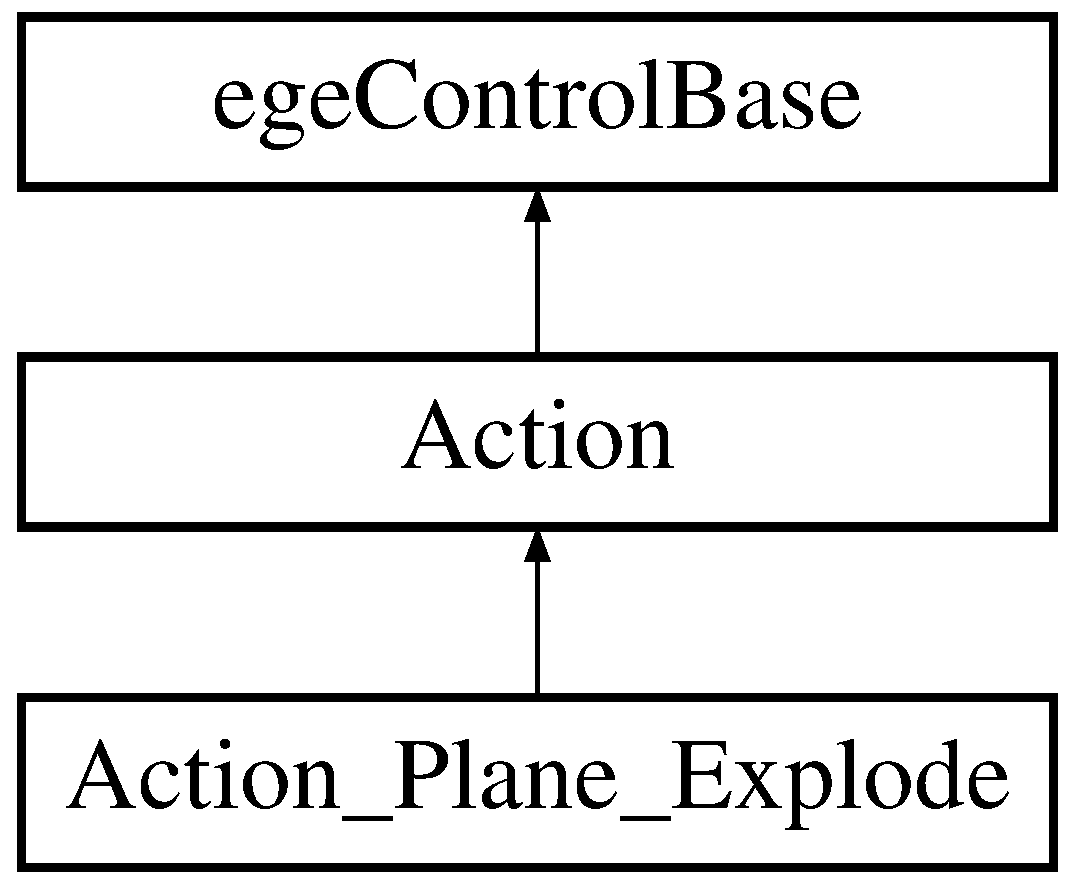
\includegraphics[height=3.000000cm]{class_action}
\end{center}
\end{figure}
\subsection*{Public 成员函数}
\begin{DoxyCompactItemize}
\item 
\mbox{\Hypertarget{class_action_a4d1309da871dfc1da7b4bdc896e34c0e}\label{class_action_a4d1309da871dfc1da7b4bdc896e34c0e}} 
{\bfseries C\+T\+L\+\_\+\+P\+R\+E\+I\+N\+IT} (\hyperlink{class_action}{Action}, ege\+Control\+Base)
\item 
\mbox{\Hypertarget{class_action_a656f4ac0205bbd055dd360248786475a}\label{class_action_a656f4ac0205bbd055dd360248786475a}} 
{\bfseries Action} (void($\ast$end\+Callback\+Func)()=N\+U\+LL, C\+T\+L\+\_\+\+D\+E\+F\+P\+A\+R\+AM)
\end{DoxyCompactItemize}
\subsection*{Public 属性}
\begin{DoxyCompactItemize}
\item 
\mbox{\Hypertarget{class_action_a682e7ba0a9ef3f891382df776c1ce883}\label{class_action_a682e7ba0a9ef3f891382df776c1ce883}} 
{\bfseries C\+T\+L\+\_\+\+P\+R\+E\+I\+N\+I\+T\+E\+ND}
\item 
\mbox{\Hypertarget{class_action_a28332e6535d45661d768bb1b321f4715}\label{class_action_a28332e6535d45661d768bb1b321f4715}} 
bool {\bfseries end}
\item 
\mbox{\Hypertarget{class_action_aef6c7c00b09ea1b0ddd7a26926309717}\label{class_action_aef6c7c00b09ea1b0ddd7a26926309717}} 
void($\ast$ {\bfseries callback} )()
\end{DoxyCompactItemize}


该类的文档由以下文件生成\+:\begin{DoxyCompactItemize}
\item 
D\+:/叶志浩文件夹/\+Vigilans的文档/\+Programming/\+Visual Studio/\+Projects/\+Grade 1 Summer Vacation/\+Lost Phoenix/\+Lost Phoenix/include/Actions.\+h\end{DoxyCompactItemize}

\hypertarget{class_action___plane___explode}{}\section{Action\+\_\+\+Plane\+\_\+\+Explode类 参考}
\label{class_action___plane___explode}\index{Action\+\_\+\+Plane\+\_\+\+Explode@{Action\+\_\+\+Plane\+\_\+\+Explode}}


{\ttfamily \#include $<$Actions.\+h$>$}

类 Action\+\_\+\+Plane\+\_\+\+Explode 继承关系图\+:\begin{figure}[H]
\begin{center}
\leavevmode
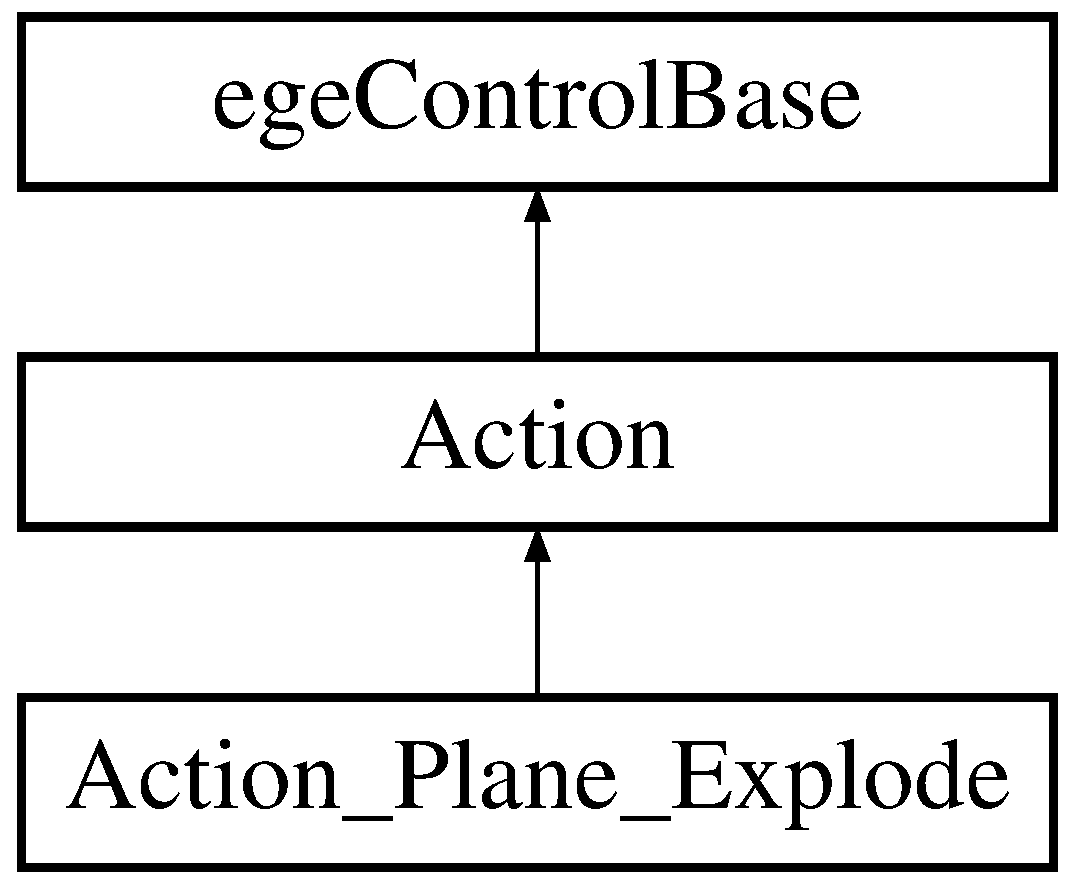
\includegraphics[height=3.000000cm]{class_action___plane___explode}
\end{center}
\end{figure}
\subsection*{Public 成员函数}
\begin{DoxyCompactItemize}
\item 
\hyperlink{class_action___plane___explode_aa7aeb998cd636ad6d0b42d9e23a43b57}{Action\+\_\+\+Plane\+\_\+\+Explode} (\hyperlink{class_plane}{Plane} $\ast$src, bool do\+Destroy=true, int boom\+Speed=5, void($\ast$end\+Callback\+Func)()=N\+U\+LL)
\item 
virtual \hyperlink{class_action___plane___explode_a1cfe86e64ece12731955275b8d6b9a41}{$\sim$\+Action\+\_\+\+Plane\+\_\+\+Explode} ()
\item 
virtual int \hyperlink{class_action___plane___explode_a1786450893420df4539056e93dcdc3b6}{on\+Update} ()
\item 
virtual void \hyperlink{class_action___plane___explode_a8436b3848df9d2f27434d5b7bebea525}{on\+Draw} (P\+I\+M\+A\+GE pimg) const
\end{DoxyCompactItemize}
\subsection*{静态 Public 成员函数}
\begin{DoxyCompactItemize}
\item 
static void \hyperlink{class_action___plane___explode_a797e8de15934ea7370086bde4cc45015}{initialize\+Models} ()
\end{DoxyCompactItemize}
\subsection*{Public 属性}
\begin{DoxyCompactItemize}
\item 
int \hyperlink{class_action___plane___explode_a3425e9988fc97a794c01b3288df4afe6}{boom\+Time}
\item 
int \hyperlink{class_action___plane___explode_a5da7d39e28db0b1a852ae81cc6e96ba5}{cur\+Index}
\item 
\hyperlink{class_plane}{Plane} $\ast$ \hyperlink{class_action___plane___explode_a98d4991b3266a6c7fc5ebbad4d41f136}{src\+Plane}
\item 
bool \hyperlink{class_action___plane___explode_a655f5cf52656c4ce16040d2310494029}{to\+Destroy}
\end{DoxyCompactItemize}
\subsection*{静态 Public 属性}
\begin{DoxyCompactItemize}
\item 
static \hyperlink{struct_texture}{Texture} \hyperlink{class_action___plane___explode_ab37c2419e1e16a739b856de09df79909}{models} \mbox{[}4\mbox{]} = \{ \}
\end{DoxyCompactItemize}


\subsection{构造及析构函数说明}
\mbox{\Hypertarget{class_action___plane___explode_aa7aeb998cd636ad6d0b42d9e23a43b57}\label{class_action___plane___explode_aa7aeb998cd636ad6d0b42d9e23a43b57}} 
\index{Action\+\_\+\+Plane\+\_\+\+Explode@{Action\+\_\+\+Plane\+\_\+\+Explode}!Action\+\_\+\+Plane\+\_\+\+Explode@{Action\+\_\+\+Plane\+\_\+\+Explode}}
\index{Action\+\_\+\+Plane\+\_\+\+Explode@{Action\+\_\+\+Plane\+\_\+\+Explode}!Action\+\_\+\+Plane\+\_\+\+Explode@{Action\+\_\+\+Plane\+\_\+\+Explode}}
\subsubsection{\texorpdfstring{Action\+\_\+\+Plane\+\_\+\+Explode()}{Action\_Plane\_Explode()}}
{\footnotesize\ttfamily Action\+\_\+\+Plane\+\_\+\+Explode\+::\+Action\+\_\+\+Plane\+\_\+\+Explode (\begin{DoxyParamCaption}\item[{\hyperlink{class_plane}{Plane} $\ast$}]{src,  }\item[{bool}]{do\+Destroy = {\ttfamily true},  }\item[{int}]{boom\+Speed = {\ttfamily 5},  }\item[{void($\ast$)()}]{end\+Callback\+Func = {\ttfamily NULL} }\end{DoxyParamCaption})}

\mbox{\Hypertarget{class_action___plane___explode_a1cfe86e64ece12731955275b8d6b9a41}\label{class_action___plane___explode_a1cfe86e64ece12731955275b8d6b9a41}} 
\index{Action\+\_\+\+Plane\+\_\+\+Explode@{Action\+\_\+\+Plane\+\_\+\+Explode}!````~Action\+\_\+\+Plane\+\_\+\+Explode@{$\sim$\+Action\+\_\+\+Plane\+\_\+\+Explode}}
\index{````~Action\+\_\+\+Plane\+\_\+\+Explode@{$\sim$\+Action\+\_\+\+Plane\+\_\+\+Explode}!Action\+\_\+\+Plane\+\_\+\+Explode@{Action\+\_\+\+Plane\+\_\+\+Explode}}
\subsubsection{\texorpdfstring{$\sim$\+Action\+\_\+\+Plane\+\_\+\+Explode()}{~Action\_Plane\_Explode()}}
{\footnotesize\ttfamily Action\+\_\+\+Plane\+\_\+\+Explode\+::$\sim$\+Action\+\_\+\+Plane\+\_\+\+Explode (\begin{DoxyParamCaption}{ }\end{DoxyParamCaption})\hspace{0.3cm}{\ttfamily [virtual]}}



\subsection{成员函数说明}
\mbox{\Hypertarget{class_action___plane___explode_a797e8de15934ea7370086bde4cc45015}\label{class_action___plane___explode_a797e8de15934ea7370086bde4cc45015}} 
\index{Action\+\_\+\+Plane\+\_\+\+Explode@{Action\+\_\+\+Plane\+\_\+\+Explode}!initialize\+Models@{initialize\+Models}}
\index{initialize\+Models@{initialize\+Models}!Action\+\_\+\+Plane\+\_\+\+Explode@{Action\+\_\+\+Plane\+\_\+\+Explode}}
\subsubsection{\texorpdfstring{initialize\+Models()}{initializeModels()}}
{\footnotesize\ttfamily void Action\+\_\+\+Plane\+\_\+\+Explode\+::initialize\+Models (\begin{DoxyParamCaption}{ }\end{DoxyParamCaption})\hspace{0.3cm}{\ttfamily [static]}}

\mbox{\Hypertarget{class_action___plane___explode_a8436b3848df9d2f27434d5b7bebea525}\label{class_action___plane___explode_a8436b3848df9d2f27434d5b7bebea525}} 
\index{Action\+\_\+\+Plane\+\_\+\+Explode@{Action\+\_\+\+Plane\+\_\+\+Explode}!on\+Draw@{on\+Draw}}
\index{on\+Draw@{on\+Draw}!Action\+\_\+\+Plane\+\_\+\+Explode@{Action\+\_\+\+Plane\+\_\+\+Explode}}
\subsubsection{\texorpdfstring{on\+Draw()}{onDraw()}}
{\footnotesize\ttfamily void Action\+\_\+\+Plane\+\_\+\+Explode\+::on\+Draw (\begin{DoxyParamCaption}\item[{P\+I\+M\+A\+GE}]{pimg }\end{DoxyParamCaption}) const\hspace{0.3cm}{\ttfamily [virtual]}}

\mbox{\Hypertarget{class_action___plane___explode_a1786450893420df4539056e93dcdc3b6}\label{class_action___plane___explode_a1786450893420df4539056e93dcdc3b6}} 
\index{Action\+\_\+\+Plane\+\_\+\+Explode@{Action\+\_\+\+Plane\+\_\+\+Explode}!on\+Update@{on\+Update}}
\index{on\+Update@{on\+Update}!Action\+\_\+\+Plane\+\_\+\+Explode@{Action\+\_\+\+Plane\+\_\+\+Explode}}
\subsubsection{\texorpdfstring{on\+Update()}{onUpdate()}}
{\footnotesize\ttfamily int Action\+\_\+\+Plane\+\_\+\+Explode\+::on\+Update (\begin{DoxyParamCaption}{ }\end{DoxyParamCaption})\hspace{0.3cm}{\ttfamily [virtual]}}



\subsection{类成员变量说明}
\mbox{\Hypertarget{class_action___plane___explode_a3425e9988fc97a794c01b3288df4afe6}\label{class_action___plane___explode_a3425e9988fc97a794c01b3288df4afe6}} 
\index{Action\+\_\+\+Plane\+\_\+\+Explode@{Action\+\_\+\+Plane\+\_\+\+Explode}!boom\+Time@{boom\+Time}}
\index{boom\+Time@{boom\+Time}!Action\+\_\+\+Plane\+\_\+\+Explode@{Action\+\_\+\+Plane\+\_\+\+Explode}}
\subsubsection{\texorpdfstring{boom\+Time}{boomTime}}
{\footnotesize\ttfamily int Action\+\_\+\+Plane\+\_\+\+Explode\+::boom\+Time}

\mbox{\Hypertarget{class_action___plane___explode_a5da7d39e28db0b1a852ae81cc6e96ba5}\label{class_action___plane___explode_a5da7d39e28db0b1a852ae81cc6e96ba5}} 
\index{Action\+\_\+\+Plane\+\_\+\+Explode@{Action\+\_\+\+Plane\+\_\+\+Explode}!cur\+Index@{cur\+Index}}
\index{cur\+Index@{cur\+Index}!Action\+\_\+\+Plane\+\_\+\+Explode@{Action\+\_\+\+Plane\+\_\+\+Explode}}
\subsubsection{\texorpdfstring{cur\+Index}{curIndex}}
{\footnotesize\ttfamily int Action\+\_\+\+Plane\+\_\+\+Explode\+::cur\+Index}

\mbox{\Hypertarget{class_action___plane___explode_ab37c2419e1e16a739b856de09df79909}\label{class_action___plane___explode_ab37c2419e1e16a739b856de09df79909}} 
\index{Action\+\_\+\+Plane\+\_\+\+Explode@{Action\+\_\+\+Plane\+\_\+\+Explode}!models@{models}}
\index{models@{models}!Action\+\_\+\+Plane\+\_\+\+Explode@{Action\+\_\+\+Plane\+\_\+\+Explode}}
\subsubsection{\texorpdfstring{models}{models}}
{\footnotesize\ttfamily \hyperlink{struct_texture}{Texture} Action\+\_\+\+Plane\+\_\+\+Explode\+::models = \{ \}\hspace{0.3cm}{\ttfamily [static]}}

\mbox{\Hypertarget{class_action___plane___explode_a98d4991b3266a6c7fc5ebbad4d41f136}\label{class_action___plane___explode_a98d4991b3266a6c7fc5ebbad4d41f136}} 
\index{Action\+\_\+\+Plane\+\_\+\+Explode@{Action\+\_\+\+Plane\+\_\+\+Explode}!src\+Plane@{src\+Plane}}
\index{src\+Plane@{src\+Plane}!Action\+\_\+\+Plane\+\_\+\+Explode@{Action\+\_\+\+Plane\+\_\+\+Explode}}
\subsubsection{\texorpdfstring{src\+Plane}{srcPlane}}
{\footnotesize\ttfamily \hyperlink{class_plane}{Plane}$\ast$ Action\+\_\+\+Plane\+\_\+\+Explode\+::src\+Plane}

\mbox{\Hypertarget{class_action___plane___explode_a655f5cf52656c4ce16040d2310494029}\label{class_action___plane___explode_a655f5cf52656c4ce16040d2310494029}} 
\index{Action\+\_\+\+Plane\+\_\+\+Explode@{Action\+\_\+\+Plane\+\_\+\+Explode}!to\+Destroy@{to\+Destroy}}
\index{to\+Destroy@{to\+Destroy}!Action\+\_\+\+Plane\+\_\+\+Explode@{Action\+\_\+\+Plane\+\_\+\+Explode}}
\subsubsection{\texorpdfstring{to\+Destroy}{toDestroy}}
{\footnotesize\ttfamily bool Action\+\_\+\+Plane\+\_\+\+Explode\+::to\+Destroy}



该类的文档由以下文件生成\+:\begin{DoxyCompactItemize}
\item 
D\+:/叶志浩文件夹/\+Vigilans的文档/\+Programming/\+Visual Studio/\+Projects/\+Grade 1 Summer Vacation/\+Lost Phoenix/\+Lost Phoenix/include/\hyperlink{_actions_8h}{Actions.\+h}\item 
D\+:/叶志浩文件夹/\+Vigilans的文档/\+Programming/\+Visual Studio/\+Projects/\+Grade 1 Summer Vacation/\+Lost Phoenix/\+Lost Phoenix/src/\hyperlink{_actions_8cpp}{Actions.\+cpp}\end{DoxyCompactItemize}

\hypertarget{struct_settings_1_1_anime_textures}{}\section{Settings\+:\+:Anime\+Textures结构体 参考}
\label{struct_settings_1_1_anime_textures}\index{Settings\+::\+Anime\+Textures@{Settings\+::\+Anime\+Textures}}


所有动画、\hyperlink{class_action}{Action}相关材质设置。  




{\ttfamily \#include $<$Resources.\+h$>$}

\subsection*{Public 属性}
\begin{DoxyCompactItemize}
\item 
\mbox{\Hypertarget{struct_settings_1_1_anime_textures_ac7d7f8216a2c1f3f06dfcb59d6ed7a10}\label{struct_settings_1_1_anime_textures_ac7d7f8216a2c1f3f06dfcb59d6ed7a10}} 
\hyperlink{struct_texture}{Texture} \hyperlink{struct_settings_1_1_anime_textures_ac7d7f8216a2c1f3f06dfcb59d6ed7a10}{explosion}
\begin{DoxyCompactList}\small\item\em 爆炸贴图材质。 \end{DoxyCompactList}\end{DoxyCompactItemize}


\subsection{详细描述}
所有动画、\hyperlink{class_action}{Action}相关材质设置。 



该结构体的文档由以下文件生成\+:\begin{DoxyCompactItemize}
\item 
D\+:/叶志浩文件夹/\+Vigilans的文档/\+Programming/\+Visual Studio/\+Projects/\+Grade 1 Summer Vacation/\+Lost Phoenix/\+Lost Phoenix/include/Resources.\+h\end{DoxyCompactItemize}

\hypertarget{structbasic__vector2_d}{}\section{basic\+\_\+vector2D$<$ \+\_\+\+Ty $>$ 模板结构体 参考}
\label{structbasic__vector2_d}\index{basic\+\_\+vector2\+D$<$ \+\_\+\+Ty $>$@{basic\+\_\+vector2\+D$<$ \+\_\+\+Ty $>$}}
\subsection*{Public 类型}
\begin{DoxyCompactItemize}
\item 
\mbox{\Hypertarget{structbasic__vector2_d_a3a8e15c6a773a34b04090604c981e63e}\label{structbasic__vector2_d_a3a8e15c6a773a34b04090604c981e63e}} 
using {\bfseries value\+\_\+type\+\_\+t} = \+\_\+\+Ty
\item 
\mbox{\Hypertarget{structbasic__vector2_d_afa9c650d6178f708c88f7abab001c4a3}\label{structbasic__vector2_d_afa9c650d6178f708c88f7abab001c4a3}} 
using {\bfseries reference\+\_\+t} = \+\_\+\+Ty \&
\end{DoxyCompactItemize}
\subsection*{Public 成员函数}
\begin{DoxyCompactItemize}
\item 
\mbox{\Hypertarget{structbasic__vector2_d_ad8b15c63d5ad6e86e1192ff820f53a67}\label{structbasic__vector2_d_ad8b15c63d5ad6e86e1192ff820f53a67}} 
{\bfseries basic\+\_\+vector2D} (\+\_\+\+Ty \+\_\+x=\+\_\+\+Ty(), \+\_\+\+Ty \+\_\+y=\+\_\+\+Ty())
\item 
\mbox{\Hypertarget{structbasic__vector2_d_a348d37f966eeda40626112688649cb70}\label{structbasic__vector2_d_a348d37f966eeda40626112688649cb70}} 
{\bfseries basic\+\_\+vector2D} (const \hyperlink{structbasic__vector2_d}{basic\+\_\+vector2D} \&a, const \hyperlink{structbasic__vector2_d}{basic\+\_\+vector2D} \&b)
\item 
\mbox{\Hypertarget{structbasic__vector2_d_a4085ab29a73798d9a1958eef96bf5f33}\label{structbasic__vector2_d_a4085ab29a73798d9a1958eef96bf5f33}} 
void {\bfseries set} (\+\_\+\+Ty \+\_\+x, \+\_\+\+Ty \+\_\+y)
\item 
\mbox{\Hypertarget{structbasic__vector2_d_a9a5e3046e0e3c08caa6bc56e6cf2d270}\label{structbasic__vector2_d_a9a5e3046e0e3c08caa6bc56e6cf2d270}} 
double {\bfseries length} ()
\item 
\mbox{\Hypertarget{structbasic__vector2_d_aa4b24c577ef24c814370beebc22f3bb8}\label{structbasic__vector2_d_aa4b24c577ef24c814370beebc22f3bb8}} 
\hyperlink{structbasic__vector2_d}{basic\+\_\+vector2D} {\bfseries unit} ()
\item 
\mbox{\Hypertarget{structbasic__vector2_d_a51f3108036d2f3df7a4d5da488717d71}\label{structbasic__vector2_d_a51f3108036d2f3df7a4d5da488717d71}} 
bool {\bfseries operator==} (const \hyperlink{structbasic__vector2_d}{basic\+\_\+vector2D} \&v2)
\item 
\mbox{\Hypertarget{structbasic__vector2_d_abd00075de4f4635651d57ede1800ad27}\label{structbasic__vector2_d_abd00075de4f4635651d57ede1800ad27}} 
bool {\bfseries operator!=} (const \hyperlink{structbasic__vector2_d}{basic\+\_\+vector2D} \&v2)
\item 
\mbox{\Hypertarget{structbasic__vector2_d_a0d01680904379f6984ee35cbe0ba3cf2}\label{structbasic__vector2_d_a0d01680904379f6984ee35cbe0ba3cf2}} 
\hyperlink{structbasic__vector2_d}{basic\+\_\+vector2D} {\bfseries operator+} (const \hyperlink{structbasic__vector2_d}{basic\+\_\+vector2D} \&v2) const
\item 
\mbox{\Hypertarget{structbasic__vector2_d_a7d335c93ec37013c5d4804bd721a04ac}\label{structbasic__vector2_d_a7d335c93ec37013c5d4804bd721a04ac}} 
\hyperlink{structbasic__vector2_d}{basic\+\_\+vector2D} {\bfseries operator-\/} (const \hyperlink{structbasic__vector2_d}{basic\+\_\+vector2D} \&v2) const
\item 
\mbox{\Hypertarget{structbasic__vector2_d_a749249ddf6d61699428d2dee790dfd9a}\label{structbasic__vector2_d_a749249ddf6d61699428d2dee790dfd9a}} 
\hyperlink{structbasic__vector2_d}{basic\+\_\+vector2D} {\bfseries operator$\ast$} (\+\_\+\+Ty scalar)
\item 
\mbox{\Hypertarget{structbasic__vector2_d_a13a6172f8b5e7308964a372ed57a794b}\label{structbasic__vector2_d_a13a6172f8b5e7308964a372ed57a794b}} 
\hyperlink{structbasic__vector2_d}{basic\+\_\+vector2D} {\bfseries operator/} (\+\_\+\+Ty scalar)
\item 
\mbox{\Hypertarget{structbasic__vector2_d_aab570d392ff446a6e16f6ca648ee65c6}\label{structbasic__vector2_d_aab570d392ff446a6e16f6ca648ee65c6}} 
\hyperlink{structbasic__vector2_d}{basic\+\_\+vector2D} \& {\bfseries operator$\ast$=} (\+\_\+\+Ty scalar)
\item 
\mbox{\Hypertarget{structbasic__vector2_d_ac608e28b6dc06bfeb28236e44bf850d0}\label{structbasic__vector2_d_ac608e28b6dc06bfeb28236e44bf850d0}} 
\hyperlink{structbasic__vector2_d}{basic\+\_\+vector2D} \& {\bfseries operator/=} (\+\_\+\+Ty scalar)
\end{DoxyCompactItemize}
\subsection*{静态 Public 成员函数}
\begin{DoxyCompactItemize}
\item 
\mbox{\Hypertarget{structbasic__vector2_d_aa31b5b9b9261d28ecd2626ba38b61278}\label{structbasic__vector2_d_aa31b5b9b9261d28ecd2626ba38b61278}} 
static \hyperlink{structbasic__vector2_d}{basic\+\_\+vector2D}$<$ double $>$ {\bfseries unit\+By\+Degree} (double degree)
\end{DoxyCompactItemize}
\subsection*{Public 属性}
\begin{DoxyCompactItemize}
\item 
\mbox{\Hypertarget{structbasic__vector2_d_a9f606d50a5993d8c8f3834e67e2e750d}\label{structbasic__vector2_d_a9f606d50a5993d8c8f3834e67e2e750d}} 
\+\_\+\+Ty {\bfseries x}
\item 
\mbox{\Hypertarget{structbasic__vector2_d_ad874ba527147096c9ee6c56ded52be73}\label{structbasic__vector2_d_ad874ba527147096c9ee6c56ded52be73}} 
\+\_\+\+Ty {\bfseries y}
\end{DoxyCompactItemize}
\subsection*{友元}
\begin{DoxyCompactItemize}
\item 
\mbox{\Hypertarget{structbasic__vector2_d_adb9aa08ea9517ddbfd6d610e270a1a0e}\label{structbasic__vector2_d_adb9aa08ea9517ddbfd6d610e270a1a0e}} 
\hyperlink{structbasic__vector2_d}{basic\+\_\+vector2D} \& {\bfseries operator+=} (\hyperlink{structbasic__vector2_d}{basic\+\_\+vector2D} \&v1, const \hyperlink{structbasic__vector2_d}{basic\+\_\+vector2D} \&v2)
\item 
\mbox{\Hypertarget{structbasic__vector2_d_a840973b019d576292fcfbb982e351314}\label{structbasic__vector2_d_a840973b019d576292fcfbb982e351314}} 
\hyperlink{structbasic__vector2_d}{basic\+\_\+vector2D} \& {\bfseries operator-\/=} (\hyperlink{structbasic__vector2_d}{basic\+\_\+vector2D} \&v1, const \hyperlink{structbasic__vector2_d}{basic\+\_\+vector2D} \&v2)
\end{DoxyCompactItemize}


该结构体的文档由以下文件生成\+:\begin{DoxyCompactItemize}
\item 
D\+:/叶志浩文件夹/\+Vigilans的文档/\+Programming/\+Visual Studio/\+Projects/\+Grade 1 Summer Vacation/\+Lost Phoenix/\+Lost Phoenix/include/Vector2\+D.\+hpp\end{DoxyCompactItemize}

\hypertarget{struct_settings_1_1_bg_textures}{}\section{Settings\+:\+:Bg\+Textures结构体 参考}
\label{struct_settings_1_1_bg_textures}\index{Settings\+::\+Bg\+Textures@{Settings\+::\+Bg\+Textures}}


{\ttfamily \#include $<$Resources.\+h$>$}

\subsection*{Public 属性}
\begin{DoxyCompactItemize}
\item 
\hyperlink{struct_texture}{Texture} \hyperlink{struct_settings_1_1_bg_textures_ab2f017635aaeb1ee5dbb544f2a053b30}{menu}
\item 
\hyperlink{struct_texture}{Texture} \hyperlink{struct_settings_1_1_bg_textures_a18b57a3e110a025b0b44ba3d838efc88}{gaming}
\item 
\hyperlink{struct_texture}{Texture} \hyperlink{struct_settings_1_1_bg_textures_ab00469bb4e54982cfffe1b7f48f593f2}{game\+Over}
\end{DoxyCompactItemize}


\subsection{类成员变量说明}
\mbox{\Hypertarget{struct_settings_1_1_bg_textures_ab00469bb4e54982cfffe1b7f48f593f2}\label{struct_settings_1_1_bg_textures_ab00469bb4e54982cfffe1b7f48f593f2}} 
\index{Settings\+::\+Bg\+Textures@{Settings\+::\+Bg\+Textures}!game\+Over@{game\+Over}}
\index{game\+Over@{game\+Over}!Settings\+::\+Bg\+Textures@{Settings\+::\+Bg\+Textures}}
\subsubsection{\texorpdfstring{game\+Over}{gameOver}}
{\footnotesize\ttfamily \hyperlink{struct_texture}{Texture} Settings\+::\+Bg\+Textures\+::game\+Over}

\mbox{\Hypertarget{struct_settings_1_1_bg_textures_a18b57a3e110a025b0b44ba3d838efc88}\label{struct_settings_1_1_bg_textures_a18b57a3e110a025b0b44ba3d838efc88}} 
\index{Settings\+::\+Bg\+Textures@{Settings\+::\+Bg\+Textures}!gaming@{gaming}}
\index{gaming@{gaming}!Settings\+::\+Bg\+Textures@{Settings\+::\+Bg\+Textures}}
\subsubsection{\texorpdfstring{gaming}{gaming}}
{\footnotesize\ttfamily \hyperlink{struct_texture}{Texture} Settings\+::\+Bg\+Textures\+::gaming}

\mbox{\Hypertarget{struct_settings_1_1_bg_textures_ab2f017635aaeb1ee5dbb544f2a053b30}\label{struct_settings_1_1_bg_textures_ab2f017635aaeb1ee5dbb544f2a053b30}} 
\index{Settings\+::\+Bg\+Textures@{Settings\+::\+Bg\+Textures}!menu@{menu}}
\index{menu@{menu}!Settings\+::\+Bg\+Textures@{Settings\+::\+Bg\+Textures}}
\subsubsection{\texorpdfstring{menu}{menu}}
{\footnotesize\ttfamily \hyperlink{struct_texture}{Texture} Settings\+::\+Bg\+Textures\+::menu}



该结构体的文档由以下文件生成\+:\begin{DoxyCompactItemize}
\item 
D\+:/叶志浩文件夹/\+Vigilans的文档/\+Programming/\+Visual Studio/\+Projects/\+Grade 1 Summer Vacation/\+Lost Phoenix/\+Lost Phoenix/include/\hyperlink{_resources_8h}{Resources.\+h}\end{DoxyCompactItemize}

\hypertarget{class_bullet}{}\section{Bullet类 参考}
\label{class_bullet}\index{Bullet@{Bullet}}
类 Bullet 继承关系图\+:\begin{figure}[H]
\begin{center}
\leavevmode
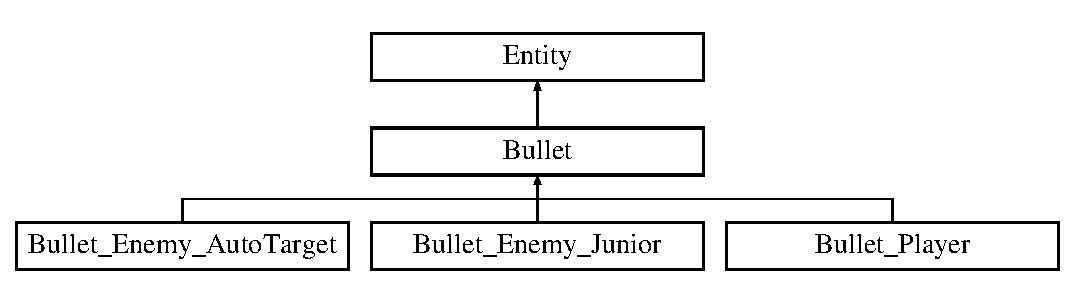
\includegraphics[height=3.000000cm]{class_bullet}
\end{center}
\end{figure}
\subsection*{Public 成员函数}
\begin{DoxyCompactItemize}
\item 
\mbox{\Hypertarget{class_bullet_ae9b56731be2ca3ff77f3a3ee4eb0bd25}\label{class_bullet_ae9b56731be2ca3ff77f3a3ee4eb0bd25}} 
{\bfseries Bullet} (\hyperlink{class_entity}{Entity} $\ast$src, \hyperlink{struct_settings_1_1_bullet}{Settings\+::\+Bullet} setting, \hyperlink{structbasic__vector2_d}{Vector2D} \hyperlink{class_entity_a386d25b56772b8913eb3e5adc636f6e0}{velocity}=\hyperlink{structbasic__vector2_d}{Vector2D}())
\item 
virtual void \hyperlink{class_bullet_a32f4a0611fe2dd245fee955d14ca1f68}{update} ()
\begin{DoxyCompactList}\small\item\em 更新实体状态。作为基类虚函数,此方法只通过速度更新当前位置。 \end{DoxyCompactList}\end{DoxyCompactItemize}
\subsection*{Public 属性}
\begin{DoxyCompactItemize}
\item 
\mbox{\Hypertarget{class_bullet_a110bd4348fc7547125b4ec4bbf94d5f5}\label{class_bullet_a110bd4348fc7547125b4ec4bbf94d5f5}} 
int {\bfseries speed}
\item 
\mbox{\Hypertarget{class_bullet_ab9e1e40341cddf25f8acc4e378b26f4a}\label{class_bullet_ab9e1e40341cddf25f8acc4e378b26f4a}} 
int {\bfseries attack}
\item 
\mbox{\Hypertarget{class_bullet_aff37198e603e1a2b8ff28e0df6e156a4}\label{class_bullet_aff37198e603e1a2b8ff28e0df6e156a4}} 
bool {\bfseries end}
\end{DoxyCompactItemize}
\subsection*{Private 成员函数}
\begin{DoxyCompactItemize}
\item 
\mbox{\Hypertarget{class_bullet_ac8350c88346ae354e7144fa20b6cb2a2}\label{class_bullet_ac8350c88346ae354e7144fa20b6cb2a2}} 
\hyperlink{structbasic__vector2_d}{Vector2D} {\bfseries init\+Pos\+By\+Source} (\hyperlink{class_entity}{Entity} $\ast$p)
\end{DoxyCompactItemize}
\subsection*{额外继承的成员函数}


\subsection{成员函数说明}
\mbox{\Hypertarget{class_bullet_a32f4a0611fe2dd245fee955d14ca1f68}\label{class_bullet_a32f4a0611fe2dd245fee955d14ca1f68}} 
\index{Bullet@{Bullet}!update@{update}}
\index{update@{update}!Bullet@{Bullet}}
\subsubsection{\texorpdfstring{update()}{update()}}
{\footnotesize\ttfamily void Bullet\+::update (\begin{DoxyParamCaption}{ }\end{DoxyParamCaption})\hspace{0.3cm}{\ttfamily [virtual]}}



更新实体状态。作为基类虚函数,此方法只通过速度更新当前位置。 



重载 \hyperlink{class_entity_a00b6eeaf99b35c8f8b10b5fbfc1baf4f}{Entity} .



该类的文档由以下文件生成\+:\begin{DoxyCompactItemize}
\item 
D\+:/叶志浩文件夹/\+Vigilans的文档/\+Programming/\+Visual Studio/\+Projects/\+Grade 1 Summer Vacation/\+Lost Phoenix/\+Lost Phoenix/include/Plane -\/ Bullet.\+h\item 
D\+:/叶志浩文件夹/\+Vigilans的文档/\+Programming/\+Visual Studio/\+Projects/\+Grade 1 Summer Vacation/\+Lost Phoenix/\+Lost Phoenix/src/Plane -\/ Bullet.\+cpp\end{DoxyCompactItemize}

\hypertarget{struct_settings_1_1_bullet}{}\section{Settings\+:\+:Bullet结构体 参考}
\label{struct_settings_1_1_bullet}\index{Settings\+::\+Bullet@{Settings\+::\+Bullet}}


子弹的设置基类。  




{\ttfamily \#include $<$Resources.\+h$>$}

\subsection*{Public 属性}
\begin{DoxyCompactItemize}
\item 
\mbox{\Hypertarget{struct_settings_1_1_bullet_a274a4b14c0bfaa540c5e60c273567bbd}\label{struct_settings_1_1_bullet_a274a4b14c0bfaa540c5e60c273567bbd}} 
\hyperlink{struct_texture}{Texture} \hyperlink{struct_settings_1_1_bullet_a274a4b14c0bfaa540c5e60c273567bbd}{texture}
\begin{DoxyCompactList}\small\item\em 子弹材质。 \end{DoxyCompactList}\item 
\mbox{\Hypertarget{struct_settings_1_1_bullet_a21e484cc6e290496e36a68da5b1a7b76}\label{struct_settings_1_1_bullet_a21e484cc6e290496e36a68da5b1a7b76}} 
int \hyperlink{struct_settings_1_1_bullet_a21e484cc6e290496e36a68da5b1a7b76}{attack}
\begin{DoxyCompactList}\small\item\em 子弹攻击力。 \end{DoxyCompactList}\item 
\mbox{\Hypertarget{struct_settings_1_1_bullet_a8969e02d4dba2f87284855e0a141f6f3}\label{struct_settings_1_1_bullet_a8969e02d4dba2f87284855e0a141f6f3}} 
int \hyperlink{struct_settings_1_1_bullet_a8969e02d4dba2f87284855e0a141f6f3}{speed}
\begin{DoxyCompactList}\small\item\em 子弹移动速率(速度的模)。 \end{DoxyCompactList}\item 
\mbox{\Hypertarget{struct_settings_1_1_bullet_aea74b608868e75f9bcf93100a38f0090}\label{struct_settings_1_1_bullet_aea74b608868e75f9bcf93100a38f0090}} 
time\+\_\+t \hyperlink{struct_settings_1_1_bullet_aea74b608868e75f9bcf93100a38f0090}{cool\+Down}
\begin{DoxyCompactList}\small\item\em 飞机射击冷却。 \end{DoxyCompactList}\end{DoxyCompactItemize}


\subsection{详细描述}
子弹的设置基类。 



该结构体的文档由以下文件生成\+:\begin{DoxyCompactItemize}
\item 
D\+:/叶志浩文件夹/\+Vigilans的文档/\+Programming/\+Visual Studio/\+Projects/\+Grade 1 Summer Vacation/\+Lost Phoenix/\+Lost Phoenix/include/\hyperlink{_resources_8h}{Resources.\+h}\end{DoxyCompactItemize}

\hypertarget{class_bullet___enemy___auto_target}{}\section{Bullet\+\_\+\+Enemy\+\_\+\+Auto\+Target类 参考}
\label{class_bullet___enemy___auto_target}\index{Bullet\+\_\+\+Enemy\+\_\+\+Auto\+Target@{Bullet\+\_\+\+Enemy\+\_\+\+Auto\+Target}}


自机狙敌机的追踪子弹。  




{\ttfamily \#include $<$Enemy\+\_\+\+Auto\+Target.\+h$>$}

类 Bullet\+\_\+\+Enemy\+\_\+\+Auto\+Target 继承关系图\+:\begin{figure}[H]
\begin{center}
\leavevmode
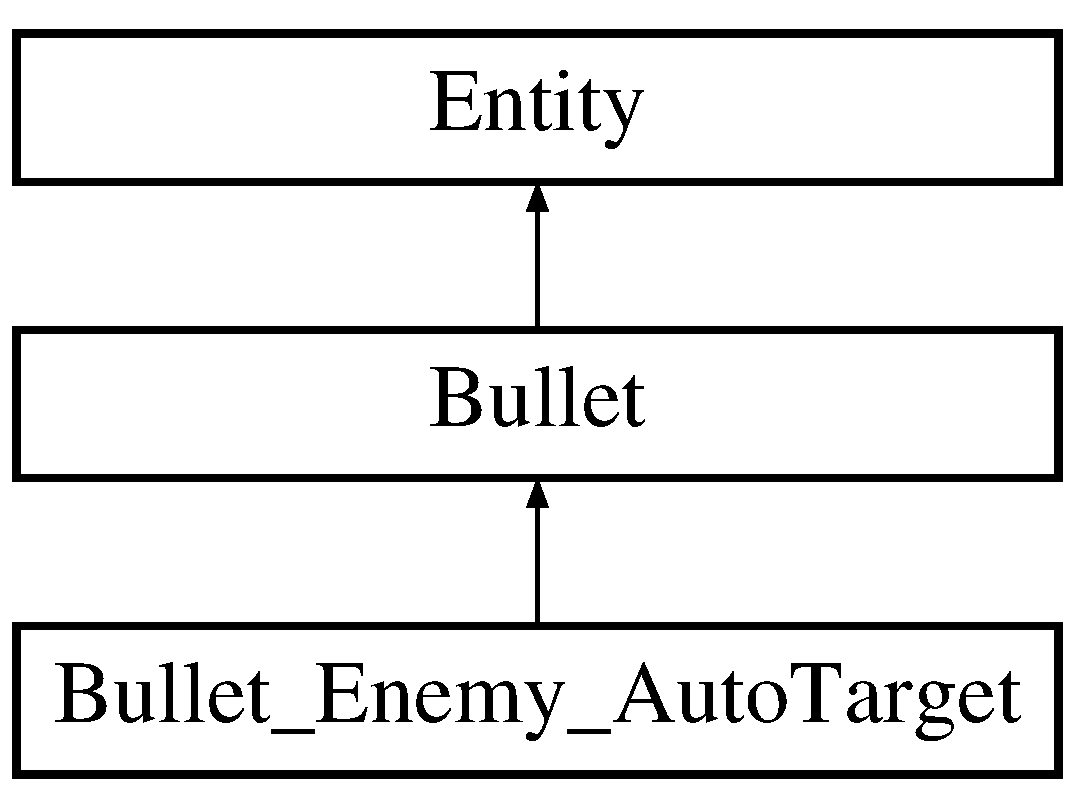
\includegraphics[height=3.000000cm]{class_bullet___enemy___auto_target}
\end{center}
\end{figure}
\subsection*{Public 成员函数}
\begin{DoxyCompactItemize}
\item 
\hyperlink{class_bullet___enemy___auto_target_ad2d9d9d8016dff0e1fd6f11c8800f314}{Bullet\+\_\+\+Enemy\+\_\+\+Auto\+Target} (\hyperlink{class_entity}{Entity} $\ast$src, \hyperlink{class_plane}{Plane} $\ast$des, \hyperlink{struct_settings_1_1_bullet}{Settings\+::\+Bullet} setting)
\begin{DoxyCompactList}\small\item\em 构造函数。 \end{DoxyCompactList}\end{DoxyCompactItemize}
\subsection*{额外继承的成员函数}


\subsection{详细描述}
自机狙敌机的追踪子弹。 

\begin{DoxySeeAlso}{参见}
T\+:\+Bullet


\end{DoxySeeAlso}


\subsection{构造及析构函数说明}
\mbox{\Hypertarget{class_bullet___enemy___auto_target_ad2d9d9d8016dff0e1fd6f11c8800f314}\label{class_bullet___enemy___auto_target_ad2d9d9d8016dff0e1fd6f11c8800f314}} 
\index{Bullet\+\_\+\+Enemy\+\_\+\+Auto\+Target@{Bullet\+\_\+\+Enemy\+\_\+\+Auto\+Target}!Bullet\+\_\+\+Enemy\+\_\+\+Auto\+Target@{Bullet\+\_\+\+Enemy\+\_\+\+Auto\+Target}}
\index{Bullet\+\_\+\+Enemy\+\_\+\+Auto\+Target@{Bullet\+\_\+\+Enemy\+\_\+\+Auto\+Target}!Bullet\+\_\+\+Enemy\+\_\+\+Auto\+Target@{Bullet\+\_\+\+Enemy\+\_\+\+Auto\+Target}}
\subsubsection{\texorpdfstring{Bullet\+\_\+\+Enemy\+\_\+\+Auto\+Target()}{Bullet\_Enemy\_AutoTarget()}}
{\footnotesize\ttfamily Bullet\+\_\+\+Enemy\+\_\+\+Auto\+Target\+::\+Bullet\+\_\+\+Enemy\+\_\+\+Auto\+Target (\begin{DoxyParamCaption}\item[{\hyperlink{class_entity}{Entity} $\ast$}]{src,  }\item[{\hyperlink{class_plane}{Plane} $\ast$}]{des,  }\item[{\hyperlink{struct_settings_1_1_bullet}{Settings\+::\+Bullet}}]{setting }\end{DoxyParamCaption})}



构造函数。 


\begin{DoxyParams}{参数}
{\em src} & 射击源 \\
\hline
{\em des} & 被追踪的飞机。一般为玩家飞机。 \\
\hline
{\em setting} & 子弹设置。 \\
\hline
\end{DoxyParams}


该类的文档由以下文件生成\+:\begin{DoxyCompactItemize}
\item 
D\+:/叶志浩文件夹/\+Vigilans的文档/\+Programming/\+Visual Studio/\+Projects/\+Grade 1 Summer Vacation/\+Lost Phoenix/\+Lost Phoenix/include/\hyperlink{_enemy___auto_target_8h}{Enemy\+\_\+\+Auto\+Target.\+h}\item 
D\+:/叶志浩文件夹/\+Vigilans的文档/\+Programming/\+Visual Studio/\+Projects/\+Grade 1 Summer Vacation/\+Lost Phoenix/\+Lost Phoenix/src/Enemy\+\_\+\+Auto\+Target.\+cpp\end{DoxyCompactItemize}

\hypertarget{class_bullet___enemy___junior}{}\section{Bullet\+\_\+\+Enemy\+\_\+\+Junior类 参考}
\label{class_bullet___enemy___junior}\index{Bullet\+\_\+\+Enemy\+\_\+\+Junior@{Bullet\+\_\+\+Enemy\+\_\+\+Junior}}


新兵敌机子弹。  




{\ttfamily \#include $<$Enemy\+\_\+\+Junior.\+h$>$}

类 Bullet\+\_\+\+Enemy\+\_\+\+Junior 继承关系图\+:\begin{figure}[H]
\begin{center}
\leavevmode
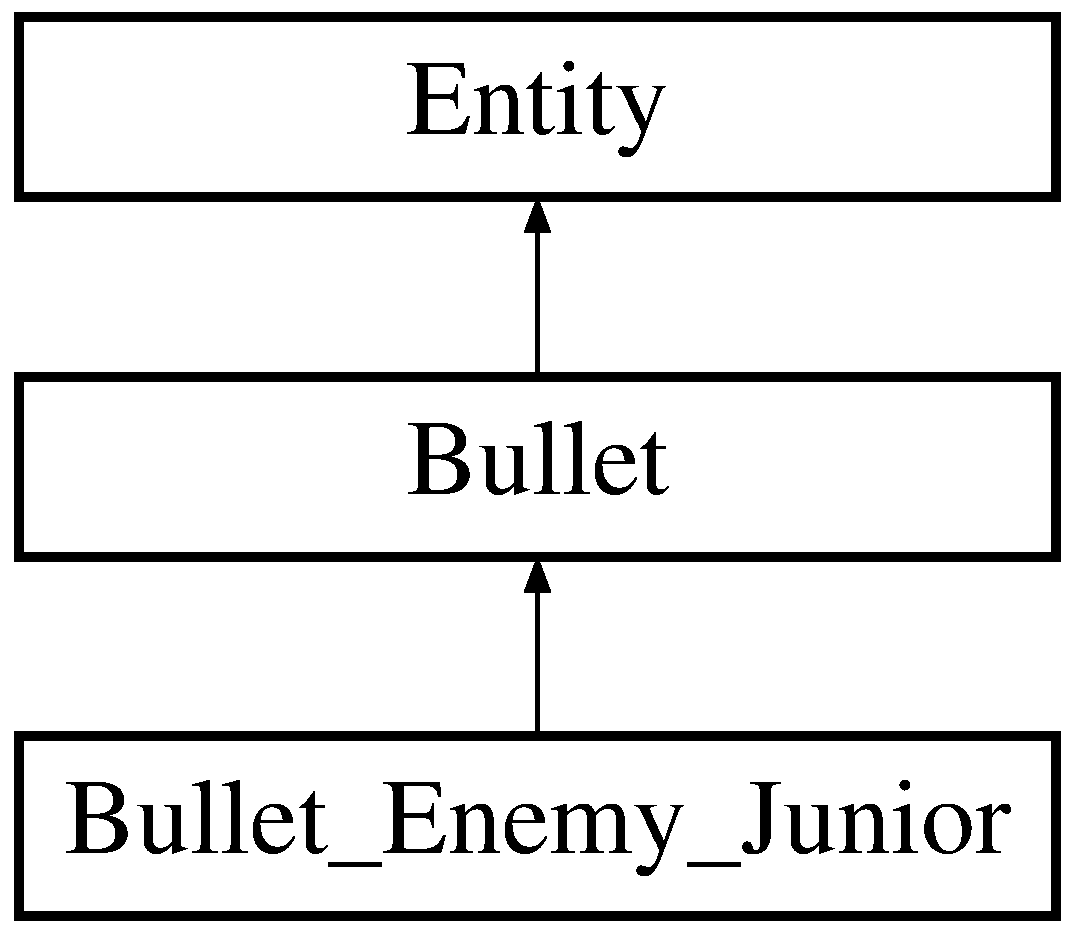
\includegraphics[height=3.000000cm]{class_bullet___enemy___junior}
\end{center}
\end{figure}
\subsection*{Public 成员函数}
\begin{DoxyCompactItemize}
\item 
\mbox{\Hypertarget{class_bullet___enemy___junior_a78eb487c660fab5536d868d7a61664eb}\label{class_bullet___enemy___junior_a78eb487c660fab5536d868d7a61664eb}} 
\hyperlink{class_bullet___enemy___junior_a78eb487c660fab5536d868d7a61664eb}{Bullet\+\_\+\+Enemy\+\_\+\+Junior} (\hyperlink{class_entity}{Entity} $\ast$src, \hyperlink{struct_settings_1_1_bullet}{Settings\+::\+Bullet} setting, \hyperlink{structbasic__vector2_d}{Vector2D} \hyperlink{class_entity_a386d25b56772b8913eb3e5adc636f6e0}{velocity}=\hyperlink{structbasic__vector2_d}{Vector2D}())
\begin{DoxyCompactList}\small\item\em 基础构造函数,与玩家子弹构造函数相同。 \end{DoxyCompactList}\end{DoxyCompactItemize}
\subsection*{额外继承的成员函数}


\subsection{详细描述}
新兵敌机子弹。 

\begin{DoxySeeAlso}{参见}
T\+:\+Bullet


\end{DoxySeeAlso}


该类的文档由以下文件生成\+:\begin{DoxyCompactItemize}
\item 
D\+:/叶志浩文件夹/\+Vigilans的文档/\+Programming/\+Visual Studio/\+Projects/\+Grade 1 Summer Vacation/\+Lost Phoenix/\+Lost Phoenix/include/Enemy\+\_\+\+Junior.\+h\item 
D\+:/叶志浩文件夹/\+Vigilans的文档/\+Programming/\+Visual Studio/\+Projects/\+Grade 1 Summer Vacation/\+Lost Phoenix/\+Lost Phoenix/src/Enemy\+\_\+\+Junior.\+cpp\end{DoxyCompactItemize}

\hypertarget{class_bullet___player}{}\section{Bullet\+\_\+\+Player类 参考}
\label{class_bullet___player}\index{Bullet\+\_\+\+Player@{Bullet\+\_\+\+Player}}


玩家飞机基础子弹。  




{\ttfamily \#include $<$Player.\+h$>$}

类 Bullet\+\_\+\+Player 继承关系图\+:\begin{figure}[H]
\begin{center}
\leavevmode
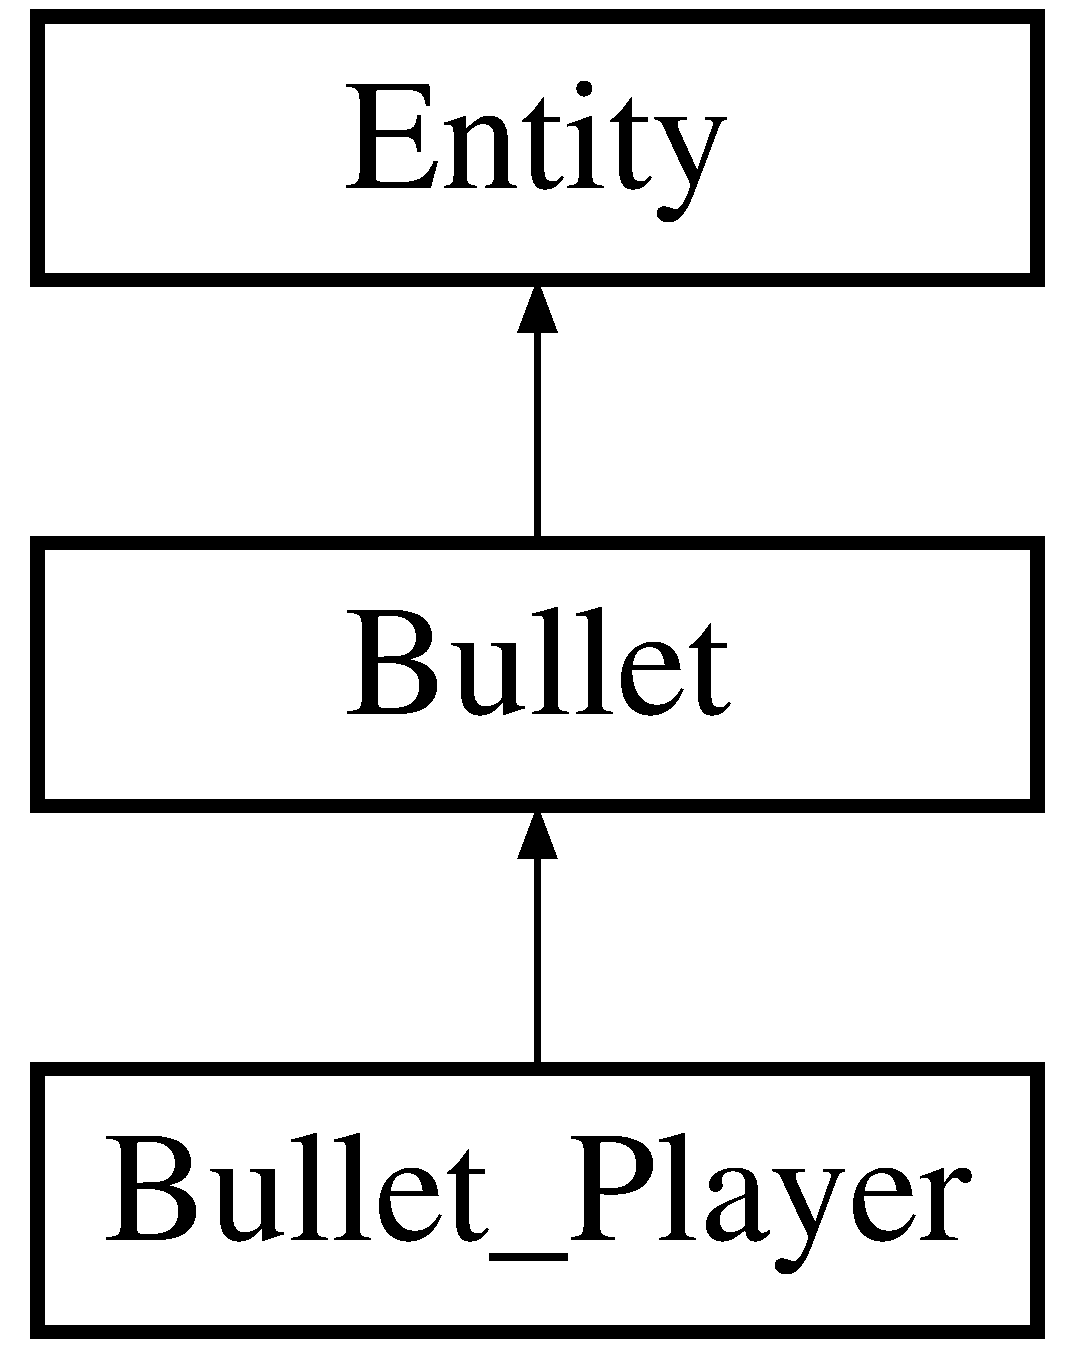
\includegraphics[height=3.000000cm]{class_bullet___player}
\end{center}
\end{figure}
\subsection*{Public 成员函数}
\begin{DoxyCompactItemize}
\item 
\hyperlink{class_bullet___player_abcb87ef10b028f5fd603c70b4cda20d3}{Bullet\+\_\+\+Player} (\hyperlink{class_entity}{Entity} $\ast$src, \hyperlink{struct_settings_1_1_bullet}{Settings\+::\+Bullet} setting, \hyperlink{structbasic__vector2_d}{Vector2D} \hyperlink{class_entity_a386d25b56772b8913eb3e5adc636f6e0}{velocity}=\hyperlink{structbasic__vector2_d}{Vector2D}())
\begin{DoxyCompactList}\small\item\em 唯一构造函数。 \end{DoxyCompactList}\end{DoxyCompactItemize}
\subsection*{额外继承的成员函数}


\subsection{详细描述}
玩家飞机基础子弹。 

\begin{DoxySeeAlso}{参见}
T\+:\+Bullet


\end{DoxySeeAlso}


\subsection{构造及析构函数说明}
\mbox{\Hypertarget{class_bullet___player_abcb87ef10b028f5fd603c70b4cda20d3}\label{class_bullet___player_abcb87ef10b028f5fd603c70b4cda20d3}} 
\index{Bullet\+\_\+\+Player@{Bullet\+\_\+\+Player}!Bullet\+\_\+\+Player@{Bullet\+\_\+\+Player}}
\index{Bullet\+\_\+\+Player@{Bullet\+\_\+\+Player}!Bullet\+\_\+\+Player@{Bullet\+\_\+\+Player}}
\subsubsection{\texorpdfstring{Bullet\+\_\+\+Player()}{Bullet\_Player()}}
{\footnotesize\ttfamily Bullet\+\_\+\+Player\+::\+Bullet\+\_\+\+Player (\begin{DoxyParamCaption}\item[{\hyperlink{class_entity}{Entity} $\ast$}]{src,  }\item[{\hyperlink{struct_settings_1_1_bullet}{Settings\+::\+Bullet}}]{setting,  }\item[{\hyperlink{structbasic__vector2_d}{Vector2D}}]{velocity = {\ttfamily \hyperlink{structbasic__vector2_d}{Vector2D}()} }\end{DoxyParamCaption})}



唯一构造函数。 


\begin{DoxyParams}{参数}
{\em src} & 射击源,一般为玩家飞机。 \\
\hline
{\em setting} & 子弹设置。 \\
\hline
{\em velocity} & 子弹速度。 \\
\hline
\end{DoxyParams}


该类的文档由以下文件生成\+:\begin{DoxyCompactItemize}
\item 
D\+:/叶志浩文件夹/\+Vigilans的文档/\+Programming/\+Visual Studio/\+Projects/\+Grade 1 Summer Vacation/\+Lost Phoenix/\+Lost Phoenix/include/Player.\+h\item 
D\+:/叶志浩文件夹/\+Vigilans的文档/\+Programming/\+Visual Studio/\+Projects/\+Grade 1 Summer Vacation/\+Lost Phoenix/\+Lost Phoenix/src/Player.\+cpp\end{DoxyCompactItemize}

\hypertarget{class_entity}{}\section{Entity类 参考}
\label{class_entity}\index{Entity@{Entity}}


游戏中所有实体的总基类。  




{\ttfamily \#include $<$Entity.\+h$>$}

类 Entity 继承关系图\+:\begin{figure}[H]
\begin{center}
\leavevmode
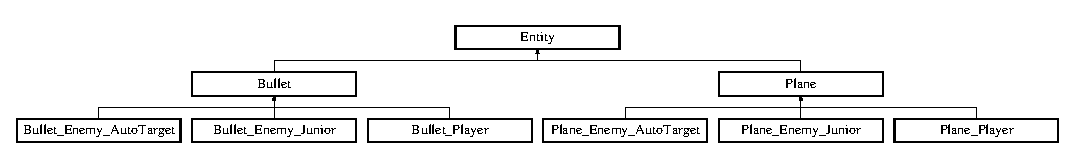
\includegraphics[height=1.686747cm]{class_entity}
\end{center}
\end{figure}
\subsection*{Public 成员函数}
\begin{DoxyCompactItemize}
\item 
\hyperlink{class_entity_a604327e36e9783d29dd6ae6e4626777a}{Entity} (\hyperlink{struct_texture}{Texture} texture, Camp \hyperlink{class_entity_a5326accd49d3817310ec90692b9da3df}{camp}, \hyperlink{structbasic__vector2_d}{Vector2D} position, \hyperlink{structbasic__vector2_d}{Vector2D} \hyperlink{class_entity_a386d25b56772b8913eb3e5adc636f6e0}{velocity}=\hyperlink{structbasic__vector2_d}{Vector2D}())
\begin{DoxyCompactList}\small\item\em 唯一构造函数。 \end{DoxyCompactList}\item 
virtual \hyperlink{class_entity_a588098978eea6a3486b7361605ff3f0f}{$\sim$\+Entity} ()
\begin{DoxyCompactList}\small\item\em 基类虚析构函数,保证子类能正常析构。 \end{DoxyCompactList}\item 
virtual void \hyperlink{class_entity_a00b6eeaf99b35c8f8b10b5fbfc1baf4f}{update} ()
\begin{DoxyCompactList}\small\item\em 更新实体状态。作为基类虚函数,此方法只通过速度更新当前位置。 \end{DoxyCompactList}\item 
virtual void \hyperlink{class_entity_a7666f416dd0d1fce0f1133f78df44476}{draw} ()
\begin{DoxyCompactList}\small\item\em 在地图上绘制实体。使用了透明通道,因此可以渲染出透明材质。 \end{DoxyCompactList}\item 
\mbox{\Hypertarget{class_entity_ac704e83937d21eb280bf0618c27e2e66}\label{class_entity_ac704e83937d21eb280bf0618c27e2e66}} 
int {\bfseries get\+X\+Pos} () const
\item 
\mbox{\Hypertarget{class_entity_a8dc5891871faff09d565738104e1d42f}\label{class_entity_a8dc5891871faff09d565738104e1d42f}} 
int {\bfseries get\+Y\+Pos} () const
\item 
\mbox{\Hypertarget{class_entity_a8afb8aa252cbbffecc2dff0669cb2896}\label{class_entity_a8afb8aa252cbbffecc2dff0669cb2896}} 
void {\bfseries set\+X\+Pos} (int x)
\item 
\mbox{\Hypertarget{class_entity_a66278a362d97e2a30912c2a31962bfb9}\label{class_entity_a66278a362d97e2a30912c2a31962bfb9}} 
void {\bfseries set\+Y\+Pos} (int y)
\item 
\mbox{\Hypertarget{class_entity_a31c55ae9457507b1c3ad5688b8f2eda2}\label{class_entity_a31c55ae9457507b1c3ad5688b8f2eda2}} 
int {\bfseries get\+X\+Vel} () const
\item 
\mbox{\Hypertarget{class_entity_abaf01d725e35883d60f1fec3f39a8ea0}\label{class_entity_abaf01d725e35883d60f1fec3f39a8ea0}} 
int {\bfseries get\+Y\+Vel} () const
\item 
\mbox{\Hypertarget{class_entity_a7f20a2190046121150e5903ec769e9dc}\label{class_entity_a7f20a2190046121150e5903ec769e9dc}} 
void {\bfseries set\+X\+Vel} (int x)
\item 
\mbox{\Hypertarget{class_entity_a9d7c4a35217e6f83ac21da314aa3ec9a}\label{class_entity_a9d7c4a35217e6f83ac21da314aa3ec9a}} 
void {\bfseries set\+Y\+Vel} (int y)
\item 
\mbox{\Hypertarget{class_entity_a5077b09978b28e502737475686ee893d}\label{class_entity_a5077b09978b28e502737475686ee893d}} 
int {\bfseries get\+X\+Hit\+Box} () const
\item 
\mbox{\Hypertarget{class_entity_ad46d1d4faf814a6b501101bc1c914754}\label{class_entity_ad46d1d4faf814a6b501101bc1c914754}} 
int {\bfseries get\+Y\+Hit\+Box} () const
\item 
\mbox{\Hypertarget{class_entity_a6086a606c751be107efdc29109346d32}\label{class_entity_a6086a606c751be107efdc29109346d32}} 
\hyperlink{structbasic__vector2_d}{Vector2D} {\bfseries get\+Position} () const
\item 
\mbox{\Hypertarget{class_entity_a3107fab87440ee7e410c4a98505dfc50}\label{class_entity_a3107fab87440ee7e410c4a98505dfc50}} 
\hyperlink{structbasic__vector2_d}{Vector2D} {\bfseries get\+Velocity} () const
\item 
\mbox{\Hypertarget{class_entity_a4d69956308b0a0396ddba314c0aa0972}\label{class_entity_a4d69956308b0a0396ddba314c0aa0972}} 
\hyperlink{structbasic__vector2_d}{Vector2D} {\bfseries get\+Hit\+Box} () const
\item 
\mbox{\Hypertarget{class_entity_a372b9155542c8a228a4f1305f5f67341}\label{class_entity_a372b9155542c8a228a4f1305f5f67341}} 
void {\bfseries set\+Position} (const \hyperlink{structbasic__vector2_d}{Vector2D} \&pos)
\item 
\mbox{\Hypertarget{class_entity_af41c73b5b2a7e68a7f285b12d0dab9f1}\label{class_entity_af41c73b5b2a7e68a7f285b12d0dab9f1}} 
void {\bfseries set\+Velocity} (const \hyperlink{structbasic__vector2_d}{Vector2D} \&vel)
\item 
\mbox{\Hypertarget{class_entity_a80b1c04df243bcdba1225a10e54995f1}\label{class_entity_a80b1c04df243bcdba1225a10e54995f1}} 
Camp {\bfseries get\+Camp} () const
\end{DoxyCompactItemize}
\subsection*{静态 Public 成员函数}
\begin{DoxyCompactItemize}
\item 
static bool \hyperlink{class_entity_afeab7f54f15446e13fbf218eccb8be53}{judge\+Collision} (const \hyperlink{class_entity}{Entity} $\ast$e1, const \hyperlink{class_entity}{Entity} $\ast$e2)
\begin{DoxyCompactList}\small\item\em 判断两个实体是否发生碰撞。 \end{DoxyCompactList}\end{DoxyCompactItemize}
\subsection*{Protected 属性}
\begin{DoxyCompactItemize}
\item 
\hyperlink{struct_texture}{Texture} \hyperlink{class_entity_a22ccba8fb86e5b4e10b2c33b6f56d238}{model}
\begin{DoxyCompactList}\small\item\em 实体的材质模型。通过它获取实体的\+Hit\+Box属性。\begin{DoxySeeAlso}{参见}
\hyperlink{struct_texture}{Texture}


\end{DoxySeeAlso}
\end{DoxyCompactList}\item 
\hyperlink{structbasic__vector2_d}{Vector2D} \hyperlink{class_entity_a5031aa6b058f2231daad16b35e3d536d}{cur\+Pos}
\begin{DoxyCompactList}\small\item\em 实体当前在地图上的位置。 \end{DoxyCompactList}\item 
\hyperlink{structbasic__vector2_d}{Vector2D} \hyperlink{class_entity_a386d25b56772b8913eb3e5adc636f6e0}{velocity}
\begin{DoxyCompactList}\small\item\em 实体当前的速度矢量。 \end{DoxyCompactList}\item 
Camp \hyperlink{class_entity_a5326accd49d3817310ec90692b9da3df}{camp}
\begin{DoxyCompactList}\small\item\em 实体当前的Camp(阵营)。 \end{DoxyCompactList}\end{DoxyCompactItemize}


\subsection{详细描述}
游戏中所有实体的总基类。 



\subsection{构造及析构函数说明}
\mbox{\Hypertarget{class_entity_a604327e36e9783d29dd6ae6e4626777a}\label{class_entity_a604327e36e9783d29dd6ae6e4626777a}} 
\index{Entity@{Entity}!Entity@{Entity}}
\index{Entity@{Entity}!Entity@{Entity}}
\subsubsection{\texorpdfstring{Entity()}{Entity()}}
{\footnotesize\ttfamily Entity\+::\+Entity (\begin{DoxyParamCaption}\item[{\hyperlink{struct_texture}{Texture}}]{texture,  }\item[{Camp}]{camp,  }\item[{\hyperlink{structbasic__vector2_d}{Vector2D}}]{position,  }\item[{\hyperlink{structbasic__vector2_d}{Vector2D}}]{velocity = {\ttfamily \hyperlink{structbasic__vector2_d}{Vector2D}()} }\end{DoxyParamCaption})\hspace{0.3cm}{\ttfamily [inline]}}



唯一构造函数。 


\begin{DoxyParams}{参数}
{\em texture} & 实体的材质。 \\
\hline
{\em camp} & 实体的Camp(阵营)。 \\
\hline
{\em position} & 实体在地图上的坐标。 \\
\hline
{\em velocity} & (可选) 实体的速度矢量。默认为0。 \\
\hline
\end{DoxyParams}
\mbox{\Hypertarget{class_entity_a588098978eea6a3486b7361605ff3f0f}\label{class_entity_a588098978eea6a3486b7361605ff3f0f}} 
\index{Entity@{Entity}!````~Entity@{$\sim$\+Entity}}
\index{````~Entity@{$\sim$\+Entity}!Entity@{Entity}}
\subsubsection{\texorpdfstring{$\sim$\+Entity()}{~Entity()}}
{\footnotesize\ttfamily virtual Entity\+::$\sim$\+Entity (\begin{DoxyParamCaption}{ }\end{DoxyParamCaption})\hspace{0.3cm}{\ttfamily [inline]}, {\ttfamily [virtual]}}



基类虚析构函数,保证子类能正常析构。 



\subsection{成员函数说明}
\mbox{\Hypertarget{class_entity_a7666f416dd0d1fce0f1133f78df44476}\label{class_entity_a7666f416dd0d1fce0f1133f78df44476}} 
\index{Entity@{Entity}!draw@{draw}}
\index{draw@{draw}!Entity@{Entity}}
\subsubsection{\texorpdfstring{draw()}{draw()}}
{\footnotesize\ttfamily void Entity\+::draw (\begin{DoxyParamCaption}{ }\end{DoxyParamCaption})\hspace{0.3cm}{\ttfamily [virtual]}}



在地图上绘制实体。使用了透明通道,因此可以渲染出透明材质。 



被 \hyperlink{class_plane_a8877358878e91929c4c01bad40cbdb78}{Plane} 重载.

\mbox{\Hypertarget{class_entity_afeab7f54f15446e13fbf218eccb8be53}\label{class_entity_afeab7f54f15446e13fbf218eccb8be53}} 
\index{Entity@{Entity}!judge\+Collision@{judge\+Collision}}
\index{judge\+Collision@{judge\+Collision}!Entity@{Entity}}
\subsubsection{\texorpdfstring{judge\+Collision()}{judgeCollision()}}
{\footnotesize\ttfamily bool Entity\+::judge\+Collision (\begin{DoxyParamCaption}\item[{const \hyperlink{class_entity}{Entity} $\ast$}]{e1,  }\item[{const \hyperlink{class_entity}{Entity} $\ast$}]{e2 }\end{DoxyParamCaption})\hspace{0.3cm}{\ttfamily [static]}}



判断两个实体是否发生碰撞。 

本来,用代码判断两个矩形是否碰撞是一件很麻烦的事……(曾经一个项目写了很长的代码但还是有问题……) 但是后来找到了一个即简单又严格的数学方法,即$\ast$$\ast$比较两个矩形重心的绝对值距离与矩形长宽的关系$\ast$$\ast$。 \begin{DoxySeeAlso}{参见}
http\+://blog.\+csdn.\+net/u011483306/article/details/45368367


\end{DoxySeeAlso}



\begin{DoxyParams}{参数}
{\em e1} & 一个实体的指针(非空)。\\
\hline
{\em e2} & 另一个实体的指针(非空)。 \\
\hline
\end{DoxyParams}
\begin{DoxyReturn}{返回}

\begin{DoxyItemize}
\item 如果发生碰撞,则返回true;
\item 如果未发生碰撞或任一参数为空,则返回false。 
\end{DoxyItemize}
\end{DoxyReturn}
\mbox{\Hypertarget{class_entity_a00b6eeaf99b35c8f8b10b5fbfc1baf4f}\label{class_entity_a00b6eeaf99b35c8f8b10b5fbfc1baf4f}} 
\index{Entity@{Entity}!update@{update}}
\index{update@{update}!Entity@{Entity}}
\subsubsection{\texorpdfstring{update()}{update()}}
{\footnotesize\ttfamily void Entity\+::update (\begin{DoxyParamCaption}{ }\end{DoxyParamCaption})\hspace{0.3cm}{\ttfamily [virtual]}}



更新实体状态。作为基类虚函数,此方法只通过速度更新当前位置。 



被 \hyperlink{class_bullet_a32f4a0611fe2dd245fee955d14ca1f68}{Bullet}, \hyperlink{class_plane_a7fbb07f76503fe057772e01f542afc32}{Plane}, \hyperlink{class_plane___player_ae68c08ce11fad9fd164c00eb4db6b348}{Plane\+\_\+\+Player}, \hyperlink{class_plane___enemy___auto_target_a79e6eda540d282205ce6151ae0b304ca}{Plane\+\_\+\+Enemy\+\_\+\+Auto\+Target} , 以及 \hyperlink{class_plane___enemy___junior_a262143737ed740f65063dbcbc5970f55}{Plane\+\_\+\+Enemy\+\_\+\+Junior} 重载.



\subsection{类成员变量说明}
\mbox{\Hypertarget{class_entity_a5326accd49d3817310ec90692b9da3df}\label{class_entity_a5326accd49d3817310ec90692b9da3df}} 
\index{Entity@{Entity}!camp@{camp}}
\index{camp@{camp}!Entity@{Entity}}
\subsubsection{\texorpdfstring{camp}{camp}}
{\footnotesize\ttfamily Camp Entity\+::camp\hspace{0.3cm}{\ttfamily [protected]}}



实体当前的Camp(阵营)。 

\mbox{\Hypertarget{class_entity_a5031aa6b058f2231daad16b35e3d536d}\label{class_entity_a5031aa6b058f2231daad16b35e3d536d}} 
\index{Entity@{Entity}!cur\+Pos@{cur\+Pos}}
\index{cur\+Pos@{cur\+Pos}!Entity@{Entity}}
\subsubsection{\texorpdfstring{cur\+Pos}{curPos}}
{\footnotesize\ttfamily \hyperlink{structbasic__vector2_d}{Vector2D} Entity\+::cur\+Pos\hspace{0.3cm}{\ttfamily [protected]}}



实体当前在地图上的位置。 

\mbox{\Hypertarget{class_entity_a22ccba8fb86e5b4e10b2c33b6f56d238}\label{class_entity_a22ccba8fb86e5b4e10b2c33b6f56d238}} 
\index{Entity@{Entity}!model@{model}}
\index{model@{model}!Entity@{Entity}}
\subsubsection{\texorpdfstring{model}{model}}
{\footnotesize\ttfamily \hyperlink{struct_texture}{Texture} Entity\+::model\hspace{0.3cm}{\ttfamily [protected]}}



实体的材质模型。通过它获取实体的\+Hit\+Box属性。\begin{DoxySeeAlso}{参见}
\hyperlink{struct_texture}{Texture}


\end{DoxySeeAlso}


\mbox{\Hypertarget{class_entity_a386d25b56772b8913eb3e5adc636f6e0}\label{class_entity_a386d25b56772b8913eb3e5adc636f6e0}} 
\index{Entity@{Entity}!velocity@{velocity}}
\index{velocity@{velocity}!Entity@{Entity}}
\subsubsection{\texorpdfstring{velocity}{velocity}}
{\footnotesize\ttfamily \hyperlink{structbasic__vector2_d}{Vector2D} Entity\+::velocity\hspace{0.3cm}{\ttfamily [protected]}}



实体当前的速度矢量。 



该类的文档由以下文件生成\+:\begin{DoxyCompactItemize}
\item 
D\+:/叶志浩文件夹/\+Vigilans的文档/\+Programming/\+Visual Studio/\+Projects/\+Grade 1 Summer Vacation/\+Lost Phoenix/\+Lost Phoenix/include/Entity.\+h\item 
D\+:/叶志浩文件夹/\+Vigilans的文档/\+Programming/\+Visual Studio/\+Projects/\+Grade 1 Summer Vacation/\+Lost Phoenix/\+Lost Phoenix/src/Entity.\+cpp\end{DoxyCompactItemize}

\hypertarget{struct_settings_1_1_general}{}\section{Settings\+:\+:General结构体 参考}
\label{struct_settings_1_1_general}\index{Settings\+::\+General@{Settings\+::\+General}}


游戏全局设置,主要包含\+U\+I与相关时间设置。  




{\ttfamily \#include $<$Resources.\+h$>$}

\subsection*{Public 属性}
\begin{DoxyCompactItemize}
\item 
\mbox{\Hypertarget{struct_settings_1_1_general_a414f100b330453215b514ec726a9fac9}\label{struct_settings_1_1_general_a414f100b330453215b514ec726a9fac9}} 
\begin{tabbing}
xx\=xx\=xx\=xx\=xx\=xx\=xx\=xx\=xx\=\kill
struct \{\\
\>char $\ast$ \hyperlink{struct_settings_1_1_general_acb5598e7641429cde268ecd8f80c4da0}{title}\\
\>\>{\em 游戏标题。 }\\
\>int \hyperlink{struct_settings_1_1_general_a5ebbaffe3220c3daf7ef79c4cd7f1ad6}{fps}\\
\>\>{\em 游戏的FPS。 }\\
\>\hyperlink{structbasic__vector2_d}{Vector2D} \hyperlink{struct_settings_1_1_general_a4cdcf50e69a10db0e410db97bd547d38}{resolution}\\
\>\>{\em 游戏窗口的分辨率。 }\\
\>int \hyperlink{struct_settings_1_1_general_ad459481ace3b01e1d80a7548325d28d2}{fontHeight}\\
\>\>{\em UI的字体高度。 }\\
\} {\bfseries UI}\\

\end{tabbing}\item 
\mbox{\Hypertarget{struct_settings_1_1_general_ae31b262693f15e6ab5ea1e1c609249b9}\label{struct_settings_1_1_general_ae31b262693f15e6ab5ea1e1c609249b9}} 
\begin{tabbing}
xx\=xx\=xx\=xx\=xx\=xx\=xx\=xx\=xx\=\kill
struct \{\\
\>time\_t \hyperlink{struct_settings_1_1_general_a4665f9d9617ebd906abbf70828c4f4f5}{enemyInfoDuration}\\
\>\>{\em 被追踪敌机的追踪状态保留时间。 }\\
\>time\_t \hyperlink{struct_settings_1_1_general_a5888b0e6d233eb4388c70b7c223552e5}{enemyWaveCoolDown}\\
\>\>{\em 敌机每一波刷新的基础冷却时间。 }\\
\>int \hyperlink{struct_settings_1_1_general_ae17ce428cf02b7c52530c8752ebca9cd}{bgShiftSpeed}\\
\>\>{\em 背景的移动速度。 }\\
\} {\bfseries times}\\

\end{tabbing}\end{DoxyCompactItemize}


\subsection{详细描述}
游戏全局设置,主要包含\+U\+I与相关时间设置。 



该结构体的文档由以下文件生成\+:\begin{DoxyCompactItemize}
\item 
D\+:/叶志浩文件夹/\+Vigilans的文档/\+Programming/\+Visual Studio/\+Projects/\+Grade 1 Summer Vacation/\+Lost Phoenix/\+Lost Phoenix/include/\hyperlink{_resources_8h}{Resources.\+h}\end{DoxyCompactItemize}

\hypertarget{class_input_controller}{}\section{Input\+Controller类 参考}
\label{class_input_controller}\index{Input\+Controller@{Input\+Controller}}


处理键盘输入的控制器类。  




{\ttfamily \#include $<$Input\+Controller.\+h$>$}

\subsection*{Public 类型}
\begin{DoxyCompactItemize}
\item 
enum \hyperlink{class_input_controller_a840a7425e2220e1ef5659a7ea4ba122d}{Key} \{ \newline
{\bfseries W}, 
{\bfseries A}, 
{\bfseries S}, 
{\bfseries D}, 
\newline
{\bfseries Space}, 
\hyperlink{class_input_controller_a840a7425e2220e1ef5659a7ea4ba122da6f6cb72d544962fa333e2e34ce64f719}{Key\+::\+Size}
 \}\begin{DoxyCompactList}\small\item\em 用来与存储键位的数组一一对应的枚举。 \end{DoxyCompactList}
\end{DoxyCompactItemize}
\subsection*{Public 成员函数}
\begin{DoxyCompactItemize}
\item 
\hyperlink{class_input_controller_aba927fffeb0bf4c4fd0835d4dfbdfaec}{Input\+Controller} ()
\begin{DoxyCompactList}\small\item\em 默认构造函数,用以初始化按键状态数组(全部置零)。 \end{DoxyCompactList}\item 
void \hyperlink{class_input_controller_a2a88542ae1370cf3f5ace3c4bb8813d9}{update\+Input} ()
\begin{DoxyCompactList}\small\item\em 从键盘更新输入。该函数会被\hyperlink{class_world_aac8c1fde63c06577ffc648aaefdb37f0}{World\+::update}调用。 \end{DoxyCompactList}\item 
bool \hyperlink{class_input_controller_a7ed265c719c06edf5a7294e98739d932}{is\+Key\+Down} (\hyperlink{class_input_controller_a840a7425e2220e1ef5659a7ea4ba122d}{Key} key)
\begin{DoxyCompactList}\small\item\em 判断当前是否按下某个键。 \end{DoxyCompactList}\end{DoxyCompactItemize}
\subsection*{Private 属性}
\begin{DoxyCompactItemize}
\item 
bool \hyperlink{class_input_controller_aebe382d8d20e579a3f2c92b58ad53ac3}{m\+\_\+\+Key\+State} \mbox{[}(int) \hyperlink{class_input_controller_a840a7425e2220e1ef5659a7ea4ba122da6f6cb72d544962fa333e2e34ce64f719}{Key\+::\+Size}\mbox{]}
\begin{DoxyCompactList}\small\item\em 存储按键状态的数组。\+Key枚举值对应元素为\hyperlink{class_input_controller_a840a7425e2220e1ef5659a7ea4ba122d}{Key}表示对应按键正被按下。 \end{DoxyCompactList}\end{DoxyCompactItemize}
\subsection*{静态 Private 属性}
\begin{DoxyCompactItemize}
\item 
static int \hyperlink{class_input_controller_afa9908a71b2107375b9104e51b465b06}{Keys\+Enum} \mbox{[}(int) \hyperlink{class_input_controller_a840a7425e2220e1ef5659a7ea4ba122da6f6cb72d544962fa333e2e34ce64f719}{Key\+::\+Size}\mbox{]} = \{\textquotesingle{}W\textquotesingle{}, \textquotesingle{}A\textquotesingle{}, \textquotesingle{}S\textquotesingle{}, \textquotesingle{}D\textquotesingle{}, V\+K\+\_\+\+S\+P\+A\+CE\}
\begin{DoxyCompactList}\small\item\em 存储某个按键对应的\+Virtual Key的数组。每个元素的索引号与\hyperlink{class_input_controller_a840a7425e2220e1ef5659a7ea4ba122d}{Key}枚举的对应枚举值一一对应。 \end{DoxyCompactList}\end{DoxyCompactItemize}


\subsection{详细描述}
处理键盘输入的控制器类。 



\subsection{成员枚举类型说明}
\mbox{\Hypertarget{class_input_controller_a840a7425e2220e1ef5659a7ea4ba122d}\label{class_input_controller_a840a7425e2220e1ef5659a7ea4ba122d}} 
\index{Input\+Controller@{Input\+Controller}!Key@{Key}}
\index{Key@{Key}!Input\+Controller@{Input\+Controller}}
\subsubsection{\texorpdfstring{Key}{Key}}
{\footnotesize\ttfamily enum \hyperlink{class_input_controller_a840a7425e2220e1ef5659a7ea4ba122d}{Input\+Controller\+::\+Key}\hspace{0.3cm}{\ttfamily [strong]}}



用来与存储键位的数组一一对应的枚举。 

\begin{DoxyEnumFields}{枚举值}
\raisebox{\heightof{T}}[0pt][0pt]{\index{Size@{Size}!Input\+Controller@{Input\+Controller}}\index{Input\+Controller@{Input\+Controller}!Size@{Size}}}\mbox{\Hypertarget{class_input_controller_a840a7425e2220e1ef5659a7ea4ba122da6f6cb72d544962fa333e2e34ce64f719}\label{class_input_controller_a840a7425e2220e1ef5659a7ea4ba122da6f6cb72d544962fa333e2e34ce64f719}} 
Size&置于枚举的最后一位,用来代表枚举拥有的元素个数(除了\+Size) \\
\hline

\end{DoxyEnumFields}


\subsection{构造及析构函数说明}
\mbox{\Hypertarget{class_input_controller_aba927fffeb0bf4c4fd0835d4dfbdfaec}\label{class_input_controller_aba927fffeb0bf4c4fd0835d4dfbdfaec}} 
\index{Input\+Controller@{Input\+Controller}!Input\+Controller@{Input\+Controller}}
\index{Input\+Controller@{Input\+Controller}!Input\+Controller@{Input\+Controller}}
\subsubsection{\texorpdfstring{Input\+Controller()}{InputController()}}
{\footnotesize\ttfamily Input\+Controller\+::\+Input\+Controller (\begin{DoxyParamCaption}{ }\end{DoxyParamCaption})}



默认构造函数,用以初始化按键状态数组(全部置零)。 



\subsection{成员函数说明}
\mbox{\Hypertarget{class_input_controller_a7ed265c719c06edf5a7294e98739d932}\label{class_input_controller_a7ed265c719c06edf5a7294e98739d932}} 
\index{Input\+Controller@{Input\+Controller}!is\+Key\+Down@{is\+Key\+Down}}
\index{is\+Key\+Down@{is\+Key\+Down}!Input\+Controller@{Input\+Controller}}
\subsubsection{\texorpdfstring{is\+Key\+Down()}{isKeyDown()}}
{\footnotesize\ttfamily bool Input\+Controller\+::is\+Key\+Down (\begin{DoxyParamCaption}\item[{\hyperlink{class_input_controller_a840a7425e2220e1ef5659a7ea4ba122d}{Key}}]{key }\end{DoxyParamCaption})}



判断当前是否按下某个键。 


\begin{DoxyParams}{参数}
{\em key} & 要检测的键位枚举值。 \\
\hline
\end{DoxyParams}
\begin{DoxyReturn}{返回}
若按下则返回真。 
\end{DoxyReturn}
\mbox{\Hypertarget{class_input_controller_a2a88542ae1370cf3f5ace3c4bb8813d9}\label{class_input_controller_a2a88542ae1370cf3f5ace3c4bb8813d9}} 
\index{Input\+Controller@{Input\+Controller}!update\+Input@{update\+Input}}
\index{update\+Input@{update\+Input}!Input\+Controller@{Input\+Controller}}
\subsubsection{\texorpdfstring{update\+Input()}{updateInput()}}
{\footnotesize\ttfamily void Input\+Controller\+::update\+Input (\begin{DoxyParamCaption}{ }\end{DoxyParamCaption})}



从键盘更新输入。该函数会被\hyperlink{class_world_aac8c1fde63c06577ffc648aaefdb37f0}{World\+::update}调用。 

此方法将遍历键盘按键消息队列,在状态数组中将对应按键状态设为true,同时将未搜索到按键的状态设为false。

时间复杂度最差为k$\ast$n, k为按键消息队列size,n为按键枚举的size。 

\subsection{类成员变量说明}
\mbox{\Hypertarget{class_input_controller_afa9908a71b2107375b9104e51b465b06}\label{class_input_controller_afa9908a71b2107375b9104e51b465b06}} 
\index{Input\+Controller@{Input\+Controller}!Keys\+Enum@{Keys\+Enum}}
\index{Keys\+Enum@{Keys\+Enum}!Input\+Controller@{Input\+Controller}}
\subsubsection{\texorpdfstring{Keys\+Enum}{KeysEnum}}
{\footnotesize\ttfamily int Input\+Controller\+::\+Keys\+Enum = \{\textquotesingle{}W\textquotesingle{}, \textquotesingle{}A\textquotesingle{}, \textquotesingle{}S\textquotesingle{}, \textquotesingle{}D\textquotesingle{}, V\+K\+\_\+\+S\+P\+A\+CE\}\hspace{0.3cm}{\ttfamily [static]}, {\ttfamily [private]}}



存储某个按键对应的\+Virtual Key的数组。每个元素的索引号与\hyperlink{class_input_controller_a840a7425e2220e1ef5659a7ea4ba122d}{Key}枚举的对应枚举值一一对应。 

\mbox{\Hypertarget{class_input_controller_aebe382d8d20e579a3f2c92b58ad53ac3}\label{class_input_controller_aebe382d8d20e579a3f2c92b58ad53ac3}} 
\index{Input\+Controller@{Input\+Controller}!m\+\_\+\+Key\+State@{m\+\_\+\+Key\+State}}
\index{m\+\_\+\+Key\+State@{m\+\_\+\+Key\+State}!Input\+Controller@{Input\+Controller}}
\subsubsection{\texorpdfstring{m\+\_\+\+Key\+State}{m\_KeyState}}
{\footnotesize\ttfamily bool Input\+Controller\+::m\+\_\+\+Key\+State\mbox{[}(int) \hyperlink{class_input_controller_a840a7425e2220e1ef5659a7ea4ba122da6f6cb72d544962fa333e2e34ce64f719}{Key\+::\+Size}\mbox{]}\hspace{0.3cm}{\ttfamily [private]}}



存储按键状态的数组。\+Key枚举值对应元素为\hyperlink{class_input_controller_a840a7425e2220e1ef5659a7ea4ba122d}{Key}表示对应按键正被按下。 



该类的文档由以下文件生成\+:\begin{DoxyCompactItemize}
\item 
D\+:/叶志浩文件夹/\+Vigilans的文档/\+Programming/\+Visual Studio/\+Projects/\+Grade 1 Summer Vacation/\+Lost Phoenix/\+Lost Phoenix/include/Input\+Controller.\+h\item 
D\+:/叶志浩文件夹/\+Vigilans的文档/\+Programming/\+Visual Studio/\+Projects/\+Grade 1 Summer Vacation/\+Lost Phoenix/\+Lost Phoenix/src/Input\+Controller.\+cpp\end{DoxyCompactItemize}

\hypertarget{class_plane}{}\section{Plane类 参考}
\label{class_plane}\index{Plane@{Plane}}


飞机的基类。  




{\ttfamily \#include $<$Plane -\/ Bullet.\+h$>$}

类 Plane 继承关系图\+:\begin{figure}[H]
\begin{center}
\leavevmode
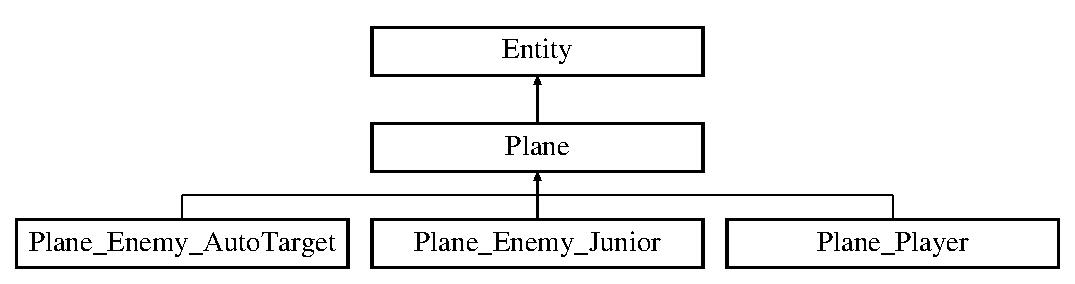
\includegraphics[height=3.000000cm]{class_plane}
\end{center}
\end{figure}
\subsection*{Public 类型}
\begin{DoxyCompactItemize}
\item 
\mbox{\Hypertarget{class_plane_a18921e108c25d0606ab76d567fcbddf1}\label{class_plane_a18921e108c25d0606ab76d567fcbddf1}} 
enum {\bfseries State} \{ {\bfseries Alive}, 
{\bfseries Dead}, 
{\bfseries Vanished}, 
{\bfseries Invincible}
 \}
\end{DoxyCompactItemize}
\subsection*{Public 成员函数}
\begin{DoxyCompactItemize}
\item 
\mbox{\Hypertarget{class_plane_ab0729538ddb380ca9a5b501f4cf72714}\label{class_plane_ab0729538ddb380ca9a5b501f4cf72714}} 
{\bfseries Plane} (\hyperlink{struct_settings_1_1_plane}{Settings\+::\+Plane} setting, \hyperlink{structbasic__vector2_d}{Vector2D} position, \hyperlink{structbasic__vector2_d}{Vector2D} \hyperlink{class_entity_a386d25b56772b8913eb3e5adc636f6e0}{velocity})
\item 
virtual void \hyperlink{class_plane_a7fbb07f76503fe057772e01f542afc32}{update} ()
\begin{DoxyCompactList}\small\item\em 更新实体状态。作为基类虚函数,此方法只通过速度更新当前位置。 \end{DoxyCompactList}\item 
virtual void \hyperlink{class_plane_a8877358878e91929c4c01bad40cbdb78}{draw} ()
\begin{DoxyCompactList}\small\item\em 在地图上绘制实体。使用了透明通道,因此可以渲染出透明材质。 \end{DoxyCompactList}\item 
\mbox{\Hypertarget{class_plane_af999499b5e79309d94004e8d012fe9c4}\label{class_plane_af999499b5e79309d94004e8d012fe9c4}} 
virtual void {\bfseries shoot} ()=0
\item 
\mbox{\Hypertarget{class_plane_a1a93dbb00292aaae274c152079f5f6f3}\label{class_plane_a1a93dbb00292aaae274c152079f5f6f3}} 
virtual void {\bfseries take\+Damage} (int damage)
\item 
\mbox{\Hypertarget{class_plane_a3cc5e05c7152c39449d36a1bf89f3e92}\label{class_plane_a3cc5e05c7152c39449d36a1bf89f3e92}} 
Plane\+::\+State {\bfseries get\+State} ()
\item 
\mbox{\Hypertarget{class_plane_a71aa431d9b6b1ab4b187ab1a24f441ff}\label{class_plane_a71aa431d9b6b1ab4b187ab1a24f441ff}} 
void {\bfseries set\+State} (Plane\+::\+State new\+\_\+state)
\item 
\mbox{\Hypertarget{class_plane_ad63d1e65ff9ca0d8b0ea1f6d37c55388}\label{class_plane_ad63d1e65ff9ca0d8b0ea1f6d37c55388}} 
int {\bfseries get\+Health} ()
\item 
\mbox{\Hypertarget{class_plane_a139404454150aac00b0f94b7f7d0d68e}\label{class_plane_a139404454150aac00b0f94b7f7d0d68e}} 
void {\bfseries set\+Health} (int hp)
\end{DoxyCompactItemize}
\subsection*{Public 属性}
\begin{DoxyCompactItemize}
\item 
\mbox{\Hypertarget{class_plane_a6ca15b26a453dfd4f81fa11a5ee278c9}\label{class_plane_a6ca15b26a453dfd4f81fa11a5ee278c9}} 
int {\bfseries speed}
\item 
\mbox{\Hypertarget{class_plane_ac39ded6721a8137c4a8044adfbfb8a6c}\label{class_plane_ac39ded6721a8137c4a8044adfbfb8a6c}} 
int {\bfseries max\+Health}
\item 
\mbox{\Hypertarget{class_plane_a0434f35fe3f56acb865e51c042e43df8}\label{class_plane_a0434f35fe3f56acb865e51c042e43df8}} 
int {\bfseries cur\+Health}
\item 
\mbox{\Hypertarget{class_plane_aee6743aa4af2550eb0581d52d0e0cafb}\label{class_plane_aee6743aa4af2550eb0581d52d0e0cafb}} 
time\+\_\+t {\bfseries shoot\+Cool\+Down}
\end{DoxyCompactItemize}
\subsection*{Protected 成员函数}
\begin{DoxyCompactItemize}
\item 
\mbox{\Hypertarget{class_plane_a77bd3df33921e215669be6583619ee45}\label{class_plane_a77bd3df33921e215669be6583619ee45}} 
bool {\bfseries check\+Shoot\+Cool\+Down} ()
\end{DoxyCompactItemize}
\subsection*{Protected 属性}
\begin{DoxyCompactItemize}
\item 
\mbox{\Hypertarget{class_plane_a04cbdef01529e67a2460f7aa4e8e6826}\label{class_plane_a04cbdef01529e67a2460f7aa4e8e6826}} 
time\+\_\+t {\bfseries shoot\+Check\+Point}
\item 
\mbox{\Hypertarget{class_plane_a15487608040be61f78e1364261f23605}\label{class_plane_a15487608040be61f78e1364261f23605}} 
Plane\+::\+State {\bfseries state}
\end{DoxyCompactItemize}
\subsection*{额外继承的成员函数}


\subsection{详细描述}
飞机的基类。 

\begin{DoxySeeAlso}{参见}
T\+:\+Entity


\end{DoxySeeAlso}


\subsection{成员函数说明}
\mbox{\Hypertarget{class_plane_a8877358878e91929c4c01bad40cbdb78}\label{class_plane_a8877358878e91929c4c01bad40cbdb78}} 
\index{Plane@{Plane}!draw@{draw}}
\index{draw@{draw}!Plane@{Plane}}
\subsubsection{\texorpdfstring{draw()}{draw()}}
{\footnotesize\ttfamily void Plane\+::draw (\begin{DoxyParamCaption}{ }\end{DoxyParamCaption})\hspace{0.3cm}{\ttfamily [virtual]}}



在地图上绘制实体。使用了透明通道,因此可以渲染出透明材质。 



重载 \hyperlink{class_entity_a7666f416dd0d1fce0f1133f78df44476}{Entity} .

\mbox{\Hypertarget{class_plane_a7fbb07f76503fe057772e01f542afc32}\label{class_plane_a7fbb07f76503fe057772e01f542afc32}} 
\index{Plane@{Plane}!update@{update}}
\index{update@{update}!Plane@{Plane}}
\subsubsection{\texorpdfstring{update()}{update()}}
{\footnotesize\ttfamily void Plane\+::update (\begin{DoxyParamCaption}{ }\end{DoxyParamCaption})\hspace{0.3cm}{\ttfamily [virtual]}}



更新实体状态。作为基类虚函数,此方法只通过速度更新当前位置。 



重载 \hyperlink{class_entity_a00b6eeaf99b35c8f8b10b5fbfc1baf4f}{Entity} .



被 \hyperlink{class_plane___player_ae68c08ce11fad9fd164c00eb4db6b348}{Plane\+\_\+\+Player}, \hyperlink{class_plane___enemy___auto_target_a79e6eda540d282205ce6151ae0b304ca}{Plane\+\_\+\+Enemy\+\_\+\+Auto\+Target} , 以及 \hyperlink{class_plane___enemy___junior_a262143737ed740f65063dbcbc5970f55}{Plane\+\_\+\+Enemy\+\_\+\+Junior} 重载.



该类的文档由以下文件生成\+:\begin{DoxyCompactItemize}
\item 
D\+:/叶志浩文件夹/\+Vigilans的文档/\+Programming/\+Visual Studio/\+Projects/\+Grade 1 Summer Vacation/\+Lost Phoenix/\+Lost Phoenix/include/Plane -\/ Bullet.\+h\item 
D\+:/叶志浩文件夹/\+Vigilans的文档/\+Programming/\+Visual Studio/\+Projects/\+Grade 1 Summer Vacation/\+Lost Phoenix/\+Lost Phoenix/src/Plane -\/ Bullet.\+cpp\end{DoxyCompactItemize}

\hypertarget{struct_settings_1_1_plane}{}\section{Settings\+:\+:Plane结构体 参考}
\label{struct_settings_1_1_plane}\index{Settings\+::\+Plane@{Settings\+::\+Plane}}


{\ttfamily \#include $<$Resources.\+h$>$}

\subsection*{Public 属性}
\begin{DoxyCompactItemize}
\item 
int \hyperlink{struct_settings_1_1_plane_a62d563a2ebc841e01bfe4737bf1fe0ab}{camp}
\item 
\hyperlink{struct_texture}{Texture} \hyperlink{struct_settings_1_1_plane_a6a000124604eb5435f4d77bbec170a4f}{texture}
\item 
int \hyperlink{struct_settings_1_1_plane_a71ffa9166855277d353d0fb6ac8f58f6}{health}
\item 
int \hyperlink{struct_settings_1_1_plane_a814ee5fe2c6b873ff4f0e0208f2c240a}{speed}
\item 
\hyperlink{struct_settings_1_1_bullet}{Bullet} \hyperlink{struct_settings_1_1_plane_a8416c74c0910b4c7a9da8d633e0c346a}{bullet\+Setting}
\item 
int \hyperlink{struct_settings_1_1_plane_a20a8861d723406f4d49610804226dd82}{score}
\end{DoxyCompactItemize}


\subsection{类成员变量说明}
\mbox{\Hypertarget{struct_settings_1_1_plane_a8416c74c0910b4c7a9da8d633e0c346a}\label{struct_settings_1_1_plane_a8416c74c0910b4c7a9da8d633e0c346a}} 
\index{Settings\+::\+Plane@{Settings\+::\+Plane}!bullet\+Setting@{bullet\+Setting}}
\index{bullet\+Setting@{bullet\+Setting}!Settings\+::\+Plane@{Settings\+::\+Plane}}
\subsubsection{\texorpdfstring{bullet\+Setting}{bulletSetting}}
{\footnotesize\ttfamily \hyperlink{struct_settings_1_1_bullet}{Bullet} Settings\+::\+Plane\+::bullet\+Setting}

\mbox{\Hypertarget{struct_settings_1_1_plane_a62d563a2ebc841e01bfe4737bf1fe0ab}\label{struct_settings_1_1_plane_a62d563a2ebc841e01bfe4737bf1fe0ab}} 
\index{Settings\+::\+Plane@{Settings\+::\+Plane}!camp@{camp}}
\index{camp@{camp}!Settings\+::\+Plane@{Settings\+::\+Plane}}
\subsubsection{\texorpdfstring{camp}{camp}}
{\footnotesize\ttfamily int Settings\+::\+Plane\+::camp}

\mbox{\Hypertarget{struct_settings_1_1_plane_a71ffa9166855277d353d0fb6ac8f58f6}\label{struct_settings_1_1_plane_a71ffa9166855277d353d0fb6ac8f58f6}} 
\index{Settings\+::\+Plane@{Settings\+::\+Plane}!health@{health}}
\index{health@{health}!Settings\+::\+Plane@{Settings\+::\+Plane}}
\subsubsection{\texorpdfstring{health}{health}}
{\footnotesize\ttfamily int Settings\+::\+Plane\+::health}

\mbox{\Hypertarget{struct_settings_1_1_plane_a20a8861d723406f4d49610804226dd82}\label{struct_settings_1_1_plane_a20a8861d723406f4d49610804226dd82}} 
\index{Settings\+::\+Plane@{Settings\+::\+Plane}!score@{score}}
\index{score@{score}!Settings\+::\+Plane@{Settings\+::\+Plane}}
\subsubsection{\texorpdfstring{score}{score}}
{\footnotesize\ttfamily int Settings\+::\+Plane\+::score}

\mbox{\Hypertarget{struct_settings_1_1_plane_a814ee5fe2c6b873ff4f0e0208f2c240a}\label{struct_settings_1_1_plane_a814ee5fe2c6b873ff4f0e0208f2c240a}} 
\index{Settings\+::\+Plane@{Settings\+::\+Plane}!speed@{speed}}
\index{speed@{speed}!Settings\+::\+Plane@{Settings\+::\+Plane}}
\subsubsection{\texorpdfstring{speed}{speed}}
{\footnotesize\ttfamily int Settings\+::\+Plane\+::speed}

\mbox{\Hypertarget{struct_settings_1_1_plane_a6a000124604eb5435f4d77bbec170a4f}\label{struct_settings_1_1_plane_a6a000124604eb5435f4d77bbec170a4f}} 
\index{Settings\+::\+Plane@{Settings\+::\+Plane}!texture@{texture}}
\index{texture@{texture}!Settings\+::\+Plane@{Settings\+::\+Plane}}
\subsubsection{\texorpdfstring{texture}{texture}}
{\footnotesize\ttfamily \hyperlink{struct_texture}{Texture} Settings\+::\+Plane\+::texture}



该结构体的文档由以下文件生成\+:\begin{DoxyCompactItemize}
\item 
D\+:/叶志浩文件夹/\+Vigilans的文档/\+Programming/\+Visual Studio/\+Projects/\+Grade 1 Summer Vacation/\+Lost Phoenix/\+Lost Phoenix/include/\hyperlink{_resources_8h}{Resources.\+h}\end{DoxyCompactItemize}

\hypertarget{class_plane___enemy___auto_target}{}\section{Plane\+\_\+\+Enemy\+\_\+\+Auto\+Target类 参考}
\label{class_plane___enemy___auto_target}\index{Plane\+\_\+\+Enemy\+\_\+\+Auto\+Target@{Plane\+\_\+\+Enemy\+\_\+\+Auto\+Target}}


{\ttfamily \#include $<$Enemy\+\_\+\+Auto\+Target.\+h$>$}

类 Plane\+\_\+\+Enemy\+\_\+\+Auto\+Target 继承关系图\+:\begin{figure}[H]
\begin{center}
\leavevmode
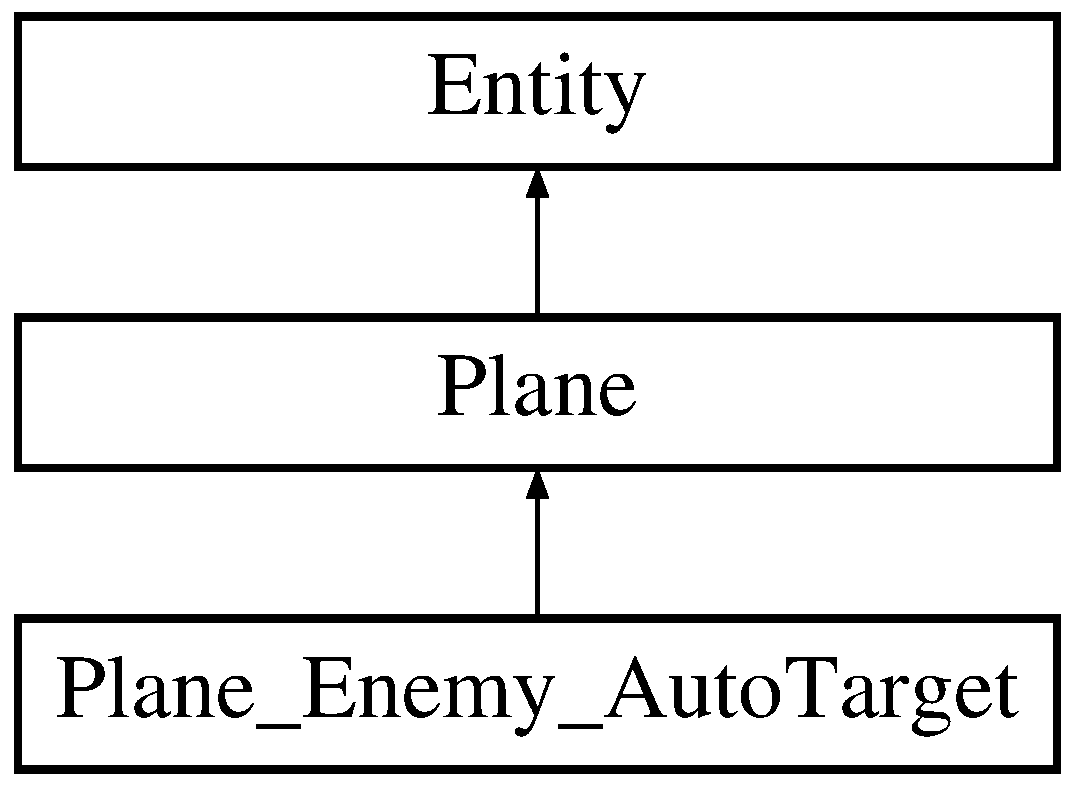
\includegraphics[height=3.000000cm]{class_plane___enemy___auto_target}
\end{center}
\end{figure}
\subsection*{Public 成员函数}
\begin{DoxyCompactItemize}
\item 
\hyperlink{class_plane___enemy___auto_target_abf4224e6d4c79583016c98dc8747f3ad}{Plane\+\_\+\+Enemy\+\_\+\+Auto\+Target} (\hyperlink{struct_settings_1_1_plane}{Settings\+::\+Plane} setting, \hyperlink{_vector2_d_8hpp_aa1f1145650f1dd9bddf7335ec6434d7c}{Vector2D} position, \hyperlink{_vector2_d_8hpp_aa1f1145650f1dd9bddf7335ec6434d7c}{Vector2D} \hyperlink{class_entity_a386d25b56772b8913eb3e5adc636f6e0}{velocity}=\hyperlink{_vector2_d_8hpp_aa1f1145650f1dd9bddf7335ec6434d7c}{Vector2D}())
\item 
virtual void \hyperlink{class_plane___enemy___auto_target_acae2a6f38bdc71d17188e2b7711f4d5b}{update} ()
\begin{DoxyCompactList}\small\item\em 更新实体状态。作为基类虚函数,此方法只通过速度更新当前位置。 \end{DoxyCompactList}\item 
virtual void \hyperlink{class_plane___enemy___auto_target_a002ba5754abc49b37ab3131f1a8f48c7}{shoot} ()
\end{DoxyCompactItemize}
\subsection*{额外继承的成员函数}


\subsection{构造及析构函数说明}
\mbox{\Hypertarget{class_plane___enemy___auto_target_abf4224e6d4c79583016c98dc8747f3ad}\label{class_plane___enemy___auto_target_abf4224e6d4c79583016c98dc8747f3ad}} 
\index{Plane\+\_\+\+Enemy\+\_\+\+Auto\+Target@{Plane\+\_\+\+Enemy\+\_\+\+Auto\+Target}!Plane\+\_\+\+Enemy\+\_\+\+Auto\+Target@{Plane\+\_\+\+Enemy\+\_\+\+Auto\+Target}}
\index{Plane\+\_\+\+Enemy\+\_\+\+Auto\+Target@{Plane\+\_\+\+Enemy\+\_\+\+Auto\+Target}!Plane\+\_\+\+Enemy\+\_\+\+Auto\+Target@{Plane\+\_\+\+Enemy\+\_\+\+Auto\+Target}}
\subsubsection{\texorpdfstring{Plane\+\_\+\+Enemy\+\_\+\+Auto\+Target()}{Plane\_Enemy\_AutoTarget()}}
{\footnotesize\ttfamily Plane\+\_\+\+Enemy\+\_\+\+Auto\+Target\+::\+Plane\+\_\+\+Enemy\+\_\+\+Auto\+Target (\begin{DoxyParamCaption}\item[{\hyperlink{struct_settings_1_1_plane}{Settings\+::\+Plane}}]{setting,  }\item[{\hyperlink{_vector2_d_8hpp_aa1f1145650f1dd9bddf7335ec6434d7c}{Vector2D}}]{position,  }\item[{\hyperlink{_vector2_d_8hpp_aa1f1145650f1dd9bddf7335ec6434d7c}{Vector2D}}]{velocity = {\ttfamily \hyperlink{_vector2_d_8hpp_aa1f1145650f1dd9bddf7335ec6434d7c}{Vector2D}()} }\end{DoxyParamCaption})}



\subsection{成员函数说明}
\mbox{\Hypertarget{class_plane___enemy___auto_target_a002ba5754abc49b37ab3131f1a8f48c7}\label{class_plane___enemy___auto_target_a002ba5754abc49b37ab3131f1a8f48c7}} 
\index{Plane\+\_\+\+Enemy\+\_\+\+Auto\+Target@{Plane\+\_\+\+Enemy\+\_\+\+Auto\+Target}!shoot@{shoot}}
\index{shoot@{shoot}!Plane\+\_\+\+Enemy\+\_\+\+Auto\+Target@{Plane\+\_\+\+Enemy\+\_\+\+Auto\+Target}}
\subsubsection{\texorpdfstring{shoot()}{shoot()}}
{\footnotesize\ttfamily void Plane\+\_\+\+Enemy\+\_\+\+Auto\+Target\+::shoot (\begin{DoxyParamCaption}{ }\end{DoxyParamCaption})\hspace{0.3cm}{\ttfamily [virtual]}}



实现了 \hyperlink{class_plane_af999499b5e79309d94004e8d012fe9c4}{Plane}.

\mbox{\Hypertarget{class_plane___enemy___auto_target_acae2a6f38bdc71d17188e2b7711f4d5b}\label{class_plane___enemy___auto_target_acae2a6f38bdc71d17188e2b7711f4d5b}} 
\index{Plane\+\_\+\+Enemy\+\_\+\+Auto\+Target@{Plane\+\_\+\+Enemy\+\_\+\+Auto\+Target}!update@{update}}
\index{update@{update}!Plane\+\_\+\+Enemy\+\_\+\+Auto\+Target@{Plane\+\_\+\+Enemy\+\_\+\+Auto\+Target}}
\subsubsection{\texorpdfstring{update()}{update()}}
{\footnotesize\ttfamily void Plane\+\_\+\+Enemy\+\_\+\+Auto\+Target\+::update (\begin{DoxyParamCaption}{ }\end{DoxyParamCaption})\hspace{0.3cm}{\ttfamily [virtual]}}



更新实体状态。作为基类虚函数,此方法只通过速度更新当前位置。 



重载 \hyperlink{class_plane_a7fbb07f76503fe057772e01f542afc32}{Plane} .



该类的文档由以下文件生成\+:\begin{DoxyCompactItemize}
\item 
D\+:/叶志浩文件夹/\+Vigilans的文档/\+Programming/\+Visual Studio/\+Projects/\+Grade 1 Summer Vacation/\+Lost Phoenix/\+Lost Phoenix/include/\hyperlink{_enemy___auto_target_8h}{Enemy\+\_\+\+Auto\+Target.\+h}\item 
D\+:/叶志浩文件夹/\+Vigilans的文档/\+Programming/\+Visual Studio/\+Projects/\+Grade 1 Summer Vacation/\+Lost Phoenix/\+Lost Phoenix/src/\hyperlink{_enemy___auto_target_8cpp}{Enemy\+\_\+\+Auto\+Target.\+cpp}\end{DoxyCompactItemize}

\hypertarget{class_plane___enemy___junior}{}\section{Plane\+\_\+\+Enemy\+\_\+\+Junior类 参考}
\label{class_plane___enemy___junior}\index{Plane\+\_\+\+Enemy\+\_\+\+Junior@{Plane\+\_\+\+Enemy\+\_\+\+Junior}}


{\ttfamily \#include $<$Enemy\+\_\+\+Junior.\+h$>$}

类 Plane\+\_\+\+Enemy\+\_\+\+Junior 继承关系图\+:\begin{figure}[H]
\begin{center}
\leavevmode
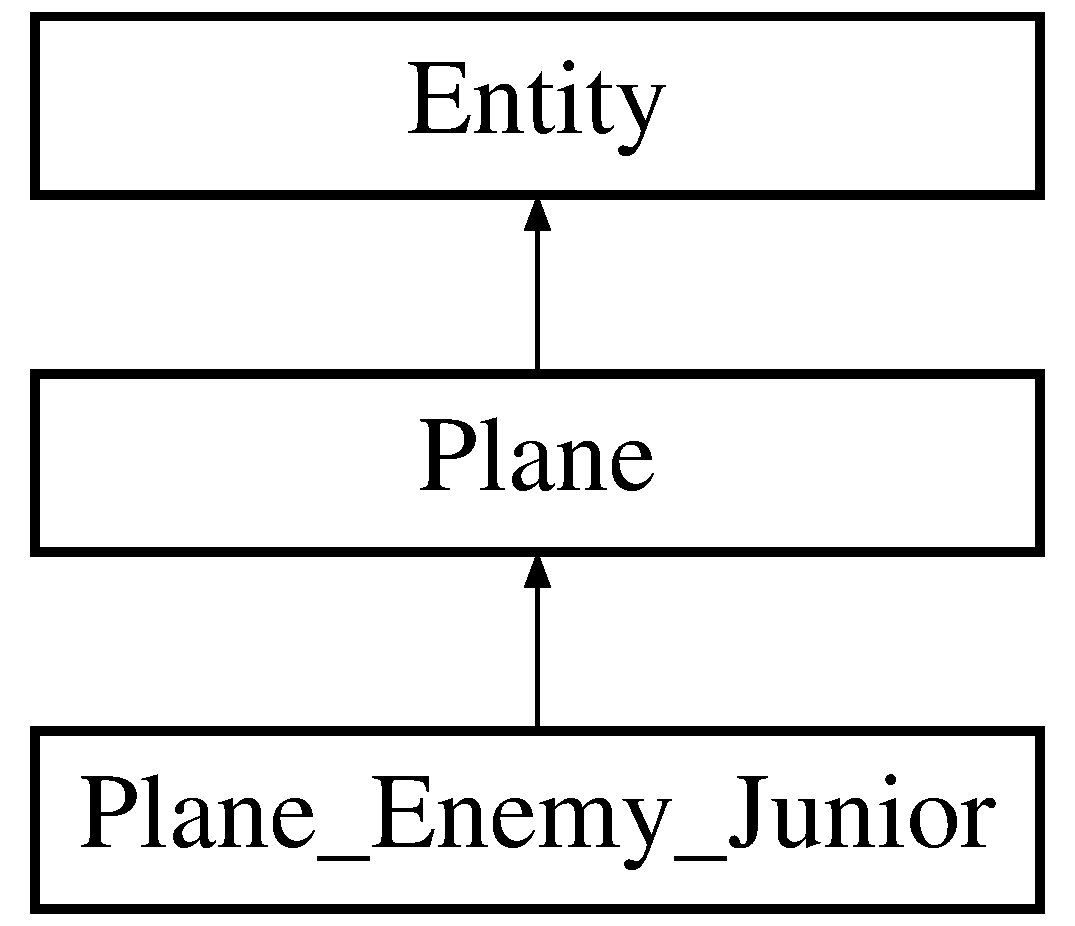
\includegraphics[height=3.000000cm]{class_plane___enemy___junior}
\end{center}
\end{figure}
\subsection*{Public 成员函数}
\begin{DoxyCompactItemize}
\item 
\hyperlink{class_plane___enemy___junior_a2a6b4a6903c05789e8be98d2d11a927d}{Plane\+\_\+\+Enemy\+\_\+\+Junior} (\hyperlink{struct_settings_1_1_plane}{Settings\+::\+Plane} setting, \hyperlink{_vector2_d_8hpp_aa1f1145650f1dd9bddf7335ec6434d7c}{Vector2D} position, \hyperlink{_vector2_d_8hpp_aa1f1145650f1dd9bddf7335ec6434d7c}{Vector2D} \hyperlink{class_entity_a386d25b56772b8913eb3e5adc636f6e0}{velocity}=\hyperlink{_vector2_d_8hpp_aa1f1145650f1dd9bddf7335ec6434d7c}{Vector2D}())
\item 
virtual void \hyperlink{class_plane___enemy___junior_a686e46c9927793dd07235cac72d52405}{update} ()
\begin{DoxyCompactList}\small\item\em 更新实体状态。作为基类虚函数,此方法只通过速度更新当前位置。 \end{DoxyCompactList}\item 
virtual void \hyperlink{class_plane___enemy___junior_ac9c3559aa4616f1b1efbe4a055fca0ac}{shoot} ()
\end{DoxyCompactItemize}
\subsection*{额外继承的成员函数}


\subsection{构造及析构函数说明}
\mbox{\Hypertarget{class_plane___enemy___junior_a2a6b4a6903c05789e8be98d2d11a927d}\label{class_plane___enemy___junior_a2a6b4a6903c05789e8be98d2d11a927d}} 
\index{Plane\+\_\+\+Enemy\+\_\+\+Junior@{Plane\+\_\+\+Enemy\+\_\+\+Junior}!Plane\+\_\+\+Enemy\+\_\+\+Junior@{Plane\+\_\+\+Enemy\+\_\+\+Junior}}
\index{Plane\+\_\+\+Enemy\+\_\+\+Junior@{Plane\+\_\+\+Enemy\+\_\+\+Junior}!Plane\+\_\+\+Enemy\+\_\+\+Junior@{Plane\+\_\+\+Enemy\+\_\+\+Junior}}
\subsubsection{\texorpdfstring{Plane\+\_\+\+Enemy\+\_\+\+Junior()}{Plane\_Enemy\_Junior()}}
{\footnotesize\ttfamily Plane\+\_\+\+Enemy\+\_\+\+Junior\+::\+Plane\+\_\+\+Enemy\+\_\+\+Junior (\begin{DoxyParamCaption}\item[{\hyperlink{struct_settings_1_1_plane}{Settings\+::\+Plane}}]{setting,  }\item[{\hyperlink{_vector2_d_8hpp_aa1f1145650f1dd9bddf7335ec6434d7c}{Vector2D}}]{position,  }\item[{\hyperlink{_vector2_d_8hpp_aa1f1145650f1dd9bddf7335ec6434d7c}{Vector2D}}]{velocity = {\ttfamily \hyperlink{_vector2_d_8hpp_aa1f1145650f1dd9bddf7335ec6434d7c}{Vector2D}()} }\end{DoxyParamCaption})}



\subsection{成员函数说明}
\mbox{\Hypertarget{class_plane___enemy___junior_ac9c3559aa4616f1b1efbe4a055fca0ac}\label{class_plane___enemy___junior_ac9c3559aa4616f1b1efbe4a055fca0ac}} 
\index{Plane\+\_\+\+Enemy\+\_\+\+Junior@{Plane\+\_\+\+Enemy\+\_\+\+Junior}!shoot@{shoot}}
\index{shoot@{shoot}!Plane\+\_\+\+Enemy\+\_\+\+Junior@{Plane\+\_\+\+Enemy\+\_\+\+Junior}}
\subsubsection{\texorpdfstring{shoot()}{shoot()}}
{\footnotesize\ttfamily void Plane\+\_\+\+Enemy\+\_\+\+Junior\+::shoot (\begin{DoxyParamCaption}{ }\end{DoxyParamCaption})\hspace{0.3cm}{\ttfamily [virtual]}}



实现了 \hyperlink{class_plane_af999499b5e79309d94004e8d012fe9c4}{Plane}.

\mbox{\Hypertarget{class_plane___enemy___junior_a686e46c9927793dd07235cac72d52405}\label{class_plane___enemy___junior_a686e46c9927793dd07235cac72d52405}} 
\index{Plane\+\_\+\+Enemy\+\_\+\+Junior@{Plane\+\_\+\+Enemy\+\_\+\+Junior}!update@{update}}
\index{update@{update}!Plane\+\_\+\+Enemy\+\_\+\+Junior@{Plane\+\_\+\+Enemy\+\_\+\+Junior}}
\subsubsection{\texorpdfstring{update()}{update()}}
{\footnotesize\ttfamily void Plane\+\_\+\+Enemy\+\_\+\+Junior\+::update (\begin{DoxyParamCaption}{ }\end{DoxyParamCaption})\hspace{0.3cm}{\ttfamily [virtual]}}



更新实体状态。作为基类虚函数,此方法只通过速度更新当前位置。 



重载 \hyperlink{class_plane_a7fbb07f76503fe057772e01f542afc32}{Plane} .



该类的文档由以下文件生成\+:\begin{DoxyCompactItemize}
\item 
D\+:/叶志浩文件夹/\+Vigilans的文档/\+Programming/\+Visual Studio/\+Projects/\+Grade 1 Summer Vacation/\+Lost Phoenix/\+Lost Phoenix/include/\hyperlink{_enemy___junior_8h}{Enemy\+\_\+\+Junior.\+h}\item 
D\+:/叶志浩文件夹/\+Vigilans的文档/\+Programming/\+Visual Studio/\+Projects/\+Grade 1 Summer Vacation/\+Lost Phoenix/\+Lost Phoenix/src/\hyperlink{_enemy___junior_8cpp}{Enemy\+\_\+\+Junior.\+cpp}\end{DoxyCompactItemize}

\hypertarget{class_plane___player}{}\section{Plane\+\_\+\+Player类 参考}
\label{class_plane___player}\index{Plane\+\_\+\+Player@{Plane\+\_\+\+Player}}


玩家飞机。  




{\ttfamily \#include $<$Player.\+h$>$}

类 Plane\+\_\+\+Player 继承关系图\+:\begin{figure}[H]
\begin{center}
\leavevmode
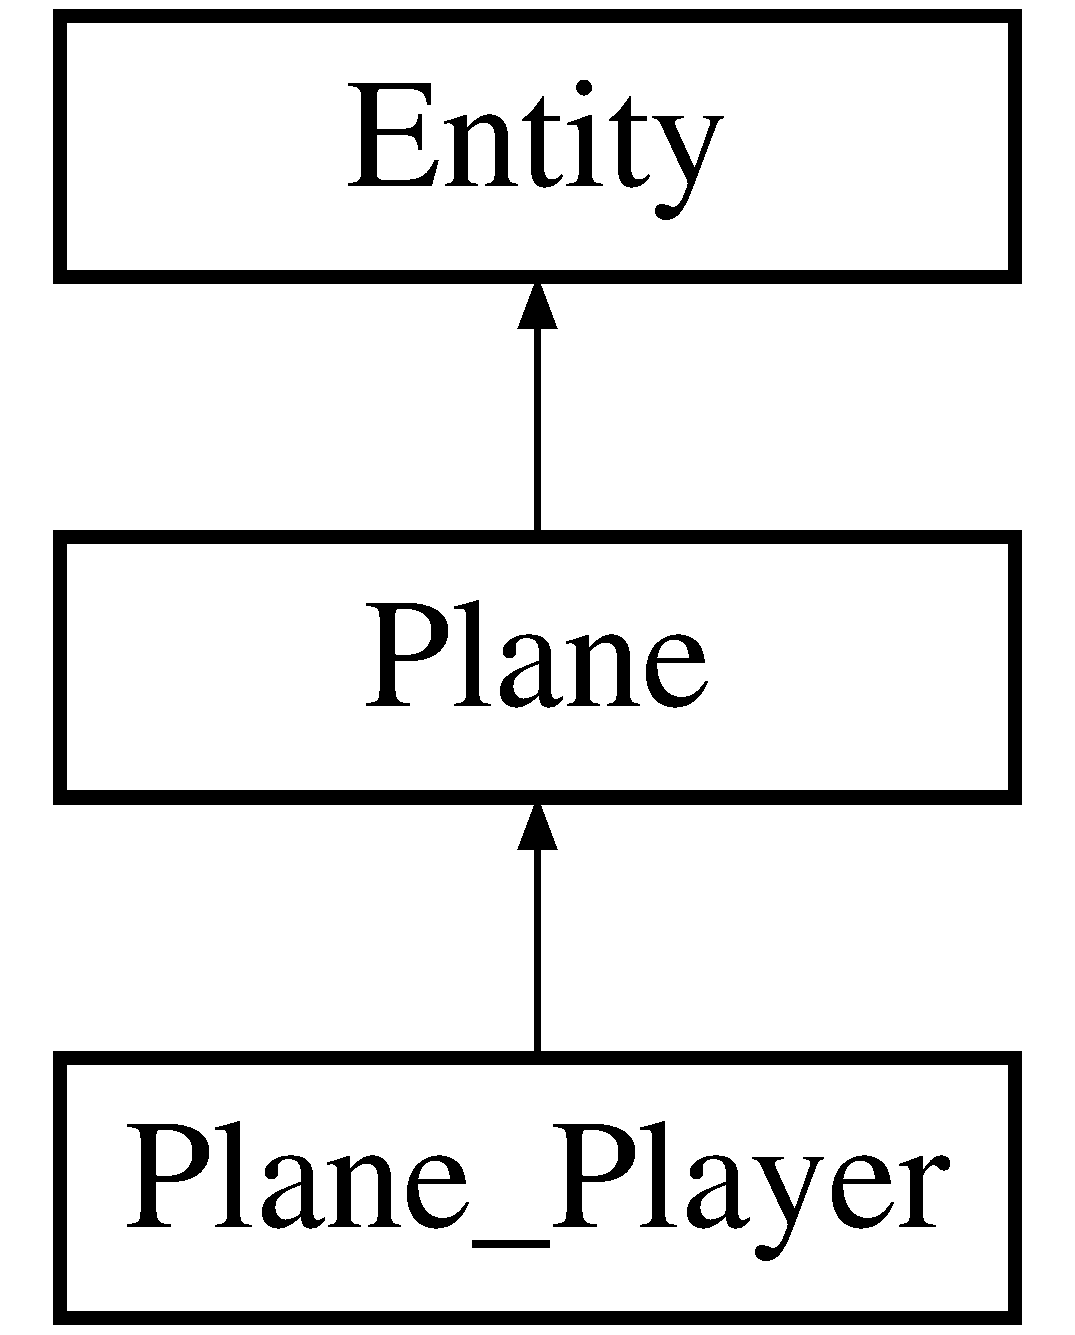
\includegraphics[height=3.000000cm]{class_plane___player}
\end{center}
\end{figure}
\subsection*{Public 成员函数}
\begin{DoxyCompactItemize}
\item 
\hyperlink{class_plane___player_ae07c92eb62cd45f7fd5d12fb570934e2}{Plane\+\_\+\+Player} (\hyperlink{struct_settings_1_1_plane}{Settings\+::\+Plane} setting)
\begin{DoxyCompactList}\small\item\em 唯一构造函数。 \end{DoxyCompactList}\item 
\mbox{\Hypertarget{class_plane___player_ae68c08ce11fad9fd164c00eb4db6b348}\label{class_plane___player_ae68c08ce11fad9fd164c00eb4db6b348}} 
virtual void \hyperlink{class_plane___player_ae68c08ce11fad9fd164c00eb4db6b348}{update} ()
\begin{DoxyCompactList}\small\item\em 更新状态,主要是更新键盘输入。若飞机已不属于存活状态,则无任何动作。 \end{DoxyCompactList}\item 
\mbox{\Hypertarget{class_plane___player_a3ffa86506370f74ec859e74d42c568c2}\label{class_plane___player_a3ffa86506370f74ec859e74d42c568c2}} 
virtual void \hyperlink{class_plane___player_a3ffa86506370f74ec859e74d42c568c2}{shoot} ()
\begin{DoxyCompactList}\small\item\em 射击,产生一个\hyperlink{class_bullet___player}{Bullet\+\_\+\+Player}。 \end{DoxyCompactList}\item 
\mbox{\Hypertarget{class_plane___player_a40e7f20858e2738e5a72b15eb1c28421}\label{class_plane___player_a40e7f20858e2738e5a72b15eb1c28421}} 
virtual void \hyperlink{class_plane___player_a40e7f20858e2738e5a72b15eb1c28421}{take\+Damage} (int damage)
\begin{DoxyCompactList}\small\item\em 承担伤害。若飞机仍存活,会产生一次\hyperlink{class_action___plane___explode}{Action\+\_\+\+Plane\+\_\+\+Explode}。 \end{DoxyCompactList}\end{DoxyCompactItemize}
\subsection*{Private 成员函数}
\begin{DoxyCompactItemize}
\item 
\mbox{\Hypertarget{class_plane___player_a7a356939196bfe1447fbd5fc03b8c380}\label{class_plane___player_a7a356939196bfe1447fbd5fc03b8c380}} 
void \hyperlink{class_plane___player_a7a356939196bfe1447fbd5fc03b8c380}{handle\+Input} ()
\begin{DoxyCompactList}\small\item\em 处理键盘输入,更新飞机状态。 \end{DoxyCompactList}\end{DoxyCompactItemize}
\subsection*{额外继承的成员函数}


\subsection{详细描述}
玩家飞机。 

\begin{DoxySeeAlso}{参见}
T\+:\+Plane


\end{DoxySeeAlso}


\subsection{构造及析构函数说明}
\mbox{\Hypertarget{class_plane___player_ae07c92eb62cd45f7fd5d12fb570934e2}\label{class_plane___player_ae07c92eb62cd45f7fd5d12fb570934e2}} 
\index{Plane\+\_\+\+Player@{Plane\+\_\+\+Player}!Plane\+\_\+\+Player@{Plane\+\_\+\+Player}}
\index{Plane\+\_\+\+Player@{Plane\+\_\+\+Player}!Plane\+\_\+\+Player@{Plane\+\_\+\+Player}}
\subsubsection{\texorpdfstring{Plane\+\_\+\+Player()}{Plane\_Player()}}
{\footnotesize\ttfamily Plane\+\_\+\+Player\+::\+Plane\+\_\+\+Player (\begin{DoxyParamCaption}\item[{\hyperlink{struct_settings_1_1_plane}{Settings\+::\+Plane}}]{setting }\end{DoxyParamCaption})}



唯一构造函数。 


\begin{DoxyParams}{参数}
{\em setting} & 飞机的设置。以后可改成{\ttfamily Settings\+::\+Player}。 \\
\hline
\end{DoxyParams}


该类的文档由以下文件生成\+:\begin{DoxyCompactItemize}
\item 
D\+:/叶志浩文件夹/\+Vigilans的文档/\+Programming/\+Visual Studio/\+Projects/\+Grade 1 Summer Vacation/\+Lost Phoenix/\+Lost Phoenix/include/\hyperlink{_player_8h}{Player.\+h}\item 
D\+:/叶志浩文件夹/\+Vigilans的文档/\+Programming/\+Visual Studio/\+Projects/\+Grade 1 Summer Vacation/\+Lost Phoenix/\+Lost Phoenix/src/Player.\+cpp\end{DoxyCompactItemize}

\hypertarget{class_resources_loader}{}\section{Resources\+Loader类 参考}
\label{class_resources_loader}\index{Resources\+Loader@{Resources\+Loader}}


资源加载器。仅在Resources.\+cpp中使用。在堆上一块稳定内存托管所有材质及设置资源。  




{\ttfamily \#include $<$Resources\+Loader.\+h$>$}

\subsection*{Public 成员函数}
\begin{DoxyCompactItemize}
\item 
\hyperlink{class_resources_loader_a571b6232d8f1dc1cf94ec752c984a834}{Resources\+Loader} ()
\begin{DoxyCompactList}\small\item\em 默认构造函数,用来在程序开始时加载所有材质设置到Texture\+Info。 \end{DoxyCompactList}\item 
\hyperlink{class_resources_loader_ab4f7fa273471e91107896131bce915da}{$\sim$\+Resources\+Loader} ()
\begin{DoxyCompactList}\small\item\em 析构函数,清除堆上所有材质及设置。 \end{DoxyCompactList}\item 
\hyperlink{struct_texture}{Texture} \hyperlink{class_resources_loader_a38cbe5a4029c4a6fe999a8405703fc30}{load\+Texture} (const wchar\+\_\+t $\ast$image\+Path, int w\+\_\+raw, int h\+\_\+raw, int w\+\_\+to=0, int h\+\_\+to=0)
\begin{DoxyCompactList}\small\item\em 通过元信息加载材质。 \end{DoxyCompactList}\item 
\hyperlink{struct_texture}{Texture} \hyperlink{class_resources_loader_a29b4b9fedb76dc01abcfacc2b31cf25c}{load\+Texture} (\hyperlink{struct_settings_1_1_texture_info}{Settings\+::\+Texture\+Info} setting)
\begin{DoxyCompactList}\small\item\em 通过Texture\+Info加载材质。 \end{DoxyCompactList}\item 
\mbox{\Hypertarget{class_resources_loader_a80e1d1bb8339e48b0becf401f205436e}\label{class_resources_loader_a80e1d1bb8339e48b0becf401f205436e}} 
void \hyperlink{class_resources_loader_a80e1d1bb8339e48b0becf401f205436e}{load\+Texture\+Settings} ()
\begin{DoxyCompactList}\small\item\em 加载所有材质设置。在程序开始时通过constructor调用。 \end{DoxyCompactList}\item 
\mbox{\Hypertarget{class_resources_loader_aae8a0b49efa4191ba01cc832c32dbd95}\label{class_resources_loader_aae8a0b49efa4191ba01cc832c32dbd95}} 
void \hyperlink{class_resources_loader_aae8a0b49efa4191ba01cc832c32dbd95}{load\+General\+Settings} ()
\begin{DoxyCompactList}\small\item\em 加载全局设置。通过\+Lazy Load机制延时调用。 \end{DoxyCompactList}\item 
\mbox{\Hypertarget{class_resources_loader_a5099528fcfd109b389965e5ebfbdb661}\label{class_resources_loader_a5099528fcfd109b389965e5ebfbdb661}} 
void \hyperlink{class_resources_loader_a5099528fcfd109b389965e5ebfbdb661}{load\+Bg\+Textures} ()
\begin{DoxyCompactList}\small\item\em 加载所有背景材质。通过\+Lazy Load机制延时调用。 \end{DoxyCompactList}\item 
\mbox{\Hypertarget{class_resources_loader_afd356d180bfc92e6135996b3d290d3ae}\label{class_resources_loader_afd356d180bfc92e6135996b3d290d3ae}} 
void \hyperlink{class_resources_loader_afd356d180bfc92e6135996b3d290d3ae}{load\+Anime\+Textures} ()
\begin{DoxyCompactList}\small\item\em 加载所有动画材质。通过\+Lazy Load机制延时调用。 \end{DoxyCompactList}\item 
\mbox{\Hypertarget{class_resources_loader_a56b70b8ad03c9fde2736d425adfd97e7}\label{class_resources_loader_a56b70b8ad03c9fde2736d425adfd97e7}} 
void \hyperlink{class_resources_loader_a56b70b8ad03c9fde2736d425adfd97e7}{load\+Plane\+Settings} ()
\begin{DoxyCompactList}\small\item\em 加载所有飞机设置。通过\+Lazy Load机制延时调用。 \end{DoxyCompactList}\item 
\mbox{\Hypertarget{class_resources_loader_afe684ff2f1419210e4bbd608c67ffeb3}\label{class_resources_loader_afe684ff2f1419210e4bbd608c67ffeb3}} 
const std\+::map$<$ int, \hyperlink{struct_texture}{Texture} $>$ \& \hyperlink{class_resources_loader_afe684ff2f1419210e4bbd608c67ffeb3}{load\+All\+Textures} ()
\begin{DoxyCompactList}\small\item\em 一次性加载所有材质。现为\+Depreciated。 \end{DoxyCompactList}\end{DoxyCompactItemize}
\subsection*{Public 属性}
\begin{DoxyCompactItemize}
\item 
\mbox{\Hypertarget{class_resources_loader_a355d825da8f96dc10cd17fc659e599ae}\label{class_resources_loader_a355d825da8f96dc10cd17fc659e599ae}} 
\begin{tabbing}
xx\=xx\=xx\=xx\=xx\=xx\=xx\=xx\=xx\=\kill
struct \{\\
\>std::unique\_ptr$<$ \hyperlink{struct_settings_1_1_general}{Settings::General} $>$ \hyperlink{class_resources_loader_a65888b4ea57a744c09dc0c9e22f9f186}{pGeneral}\\
\>\>{\em 默认全局设置。 }\\
\>std::unique\_ptr$<$ \hyperlink{struct_settings_1_1_bg_textures}{Settings::BgTextures} $>$ \hyperlink{class_resources_loader_aada194614a803df2a3680e5c5992a18a}{pBgTextures}\\
\>\>{\em 所有背景材质。 }\\
\>std::unique\_ptr$<$ \hyperlink{struct_settings_1_1_anime_textures}{Settings::AnimeTextures} $>$ \hyperlink{class_resources_loader_a72df15c8b925035fda4edfeb52830d82}{pAnimeTextures}\\
\>\>{\em 所有动画材质。 }\\
\>std::unique\_ptr$<$ \hyperlink{struct_settings_1_1_plane}{Settings::Plane} $>$ \hyperlink{class_resources_loader_ae874a55d363c3cb651f36e47570d30a9}{pPlayer}\\
\>\>{\em 默认玩家飞机设置。 }\\
\>std::unique\_ptr$<$ \hyperlink{struct_settings_1_1_plane}{Settings::Plane} $>$ \hyperlink{class_resources_loader_a150dacb6180f32ab8fafadcefdc65f96}{pEnemyJunior}\\
\>\>{\em 默认新兵敌机设置。 }\\
\>std::unique\_ptr$<$ \hyperlink{struct_settings_1_1_plane}{Settings::Plane} $>$ \hyperlink{class_resources_loader_a99ac5605a8b7fedb9c79b3f6b6d310cb}{pEnemyAutoTarget}\\
\>\>{\em 默认自机狙敌机设置。 }\\
\>std::map$<$ int, \hyperlink{struct_settings_1_1_texture_info}{Settings::TextureInfo} $>$ \hyperlink{class_resources_loader_ae364e855ac860a1404ddf324b0ef0300}{mTextureInfos}\\
\>\>{\em 保存所有材质索引设置。 }\\
\} \hyperlink{class_resources_loader_a355d825da8f96dc10cd17fc659e599ae}{settings}\\

\end{tabbing}\begin{DoxyCompactList}\small\item\em 保存所有默认设置。所有外部类通过此处保存的设置的引用来获取默认设置。 \end{DoxyCompactList}\item 
\mbox{\Hypertarget{class_resources_loader_a5b18435b040ae9562a84570712be922c}\label{class_resources_loader_a5b18435b040ae9562a84570712be922c}} 
std\+::map$<$ int, \hyperlink{struct_texture}{Texture} $>$ \hyperlink{class_resources_loader_a5b18435b040ae9562a84570712be922c}{textures}
\begin{DoxyCompactList}\small\item\em 保存所有已完整加载的材质。通过材质的\+I\+D进行检索。 \end{DoxyCompactList}\end{DoxyCompactItemize}


\subsection{详细描述}
资源加载器。仅在Resources.\+cpp中使用。在堆上一块稳定内存托管所有材质及设置资源。 



\subsection{构造及析构函数说明}
\mbox{\Hypertarget{class_resources_loader_a571b6232d8f1dc1cf94ec752c984a834}\label{class_resources_loader_a571b6232d8f1dc1cf94ec752c984a834}} 
\index{Resources\+Loader@{Resources\+Loader}!Resources\+Loader@{Resources\+Loader}}
\index{Resources\+Loader@{Resources\+Loader}!Resources\+Loader@{Resources\+Loader}}
\subsubsection{\texorpdfstring{Resources\+Loader()}{ResourcesLoader()}}
{\footnotesize\ttfamily Resources\+Loader\+::\+Resources\+Loader (\begin{DoxyParamCaption}{ }\end{DoxyParamCaption})}



默认构造函数,用来在程序开始时加载所有材质设置到Texture\+Info。 

\mbox{\Hypertarget{class_resources_loader_ab4f7fa273471e91107896131bce915da}\label{class_resources_loader_ab4f7fa273471e91107896131bce915da}} 
\index{Resources\+Loader@{Resources\+Loader}!````~Resources\+Loader@{$\sim$\+Resources\+Loader}}
\index{````~Resources\+Loader@{$\sim$\+Resources\+Loader}!Resources\+Loader@{Resources\+Loader}}
\subsubsection{\texorpdfstring{$\sim$\+Resources\+Loader()}{~ResourcesLoader()}}
{\footnotesize\ttfamily Resources\+Loader\+::$\sim$\+Resources\+Loader (\begin{DoxyParamCaption}{ }\end{DoxyParamCaption})}



析构函数,清除堆上所有材质及设置。 



\subsection{成员函数说明}
\mbox{\Hypertarget{class_resources_loader_a38cbe5a4029c4a6fe999a8405703fc30}\label{class_resources_loader_a38cbe5a4029c4a6fe999a8405703fc30}} 
\index{Resources\+Loader@{Resources\+Loader}!load\+Texture@{load\+Texture}}
\index{load\+Texture@{load\+Texture}!Resources\+Loader@{Resources\+Loader}}
\subsubsection{\texorpdfstring{load\+Texture()}{loadTexture()}\hspace{0.1cm}{\footnotesize\ttfamily [1/2]}}
{\footnotesize\ttfamily \hyperlink{struct_texture}{Texture} Resources\+Loader\+::load\+Texture (\begin{DoxyParamCaption}\item[{const wchar\+\_\+t $\ast$}]{image\+Path,  }\item[{int}]{w\+\_\+raw,  }\item[{int}]{h\+\_\+raw,  }\item[{int}]{w\+\_\+to = {\ttfamily 0},  }\item[{int}]{h\+\_\+to = {\ttfamily 0} }\end{DoxyParamCaption})}



通过元信息加载材质。 

当w\+\_\+to或h\+\_\+to中有任意一项为0时,表示不缩放。 


\begin{DoxyParams}{参数}
{\em image\+Path} & 材质的路径,采用\+Unicode。 \\
\hline
{\em w\+\_\+raw} & 材质的原分辨率宽度。 \\
\hline
{\em h\+\_\+raw} & 材质的原分辨率高度。 \\
\hline
{\em w\+\_\+to} & (可选) 期望缩放到的分辨率宽度。 \\
\hline
{\em h\+\_\+to} & (可选) 期望缩放到的分辨率高度。 \\
\hline
\end{DoxyParams}
\begin{DoxyReturn}{返回}
加载成功后,返回加载而得的材质。 
\end{DoxyReturn}
\mbox{\Hypertarget{class_resources_loader_a29b4b9fedb76dc01abcfacc2b31cf25c}\label{class_resources_loader_a29b4b9fedb76dc01abcfacc2b31cf25c}} 
\index{Resources\+Loader@{Resources\+Loader}!load\+Texture@{load\+Texture}}
\index{load\+Texture@{load\+Texture}!Resources\+Loader@{Resources\+Loader}}
\subsubsection{\texorpdfstring{load\+Texture()}{loadTexture()}\hspace{0.1cm}{\footnotesize\ttfamily [2/2]}}
{\footnotesize\ttfamily \hyperlink{struct_texture}{Texture} Resources\+Loader\+::load\+Texture (\begin{DoxyParamCaption}\item[{\hyperlink{struct_settings_1_1_texture_info}{Settings\+::\+Texture\+Info}}]{setting }\end{DoxyParamCaption})\hspace{0.3cm}{\ttfamily [inline]}}



通过Texture\+Info加载材质。 

封装了一个接收材质设置的更良好的接口。在类体中定义是默认inline的。

T\+O\+DO\+: 用参数转发(forwarding)实现这个重载。 


\begin{DoxyParams}{参数}
{\em setting} & 材质的设置源。 \\
\hline
\end{DoxyParams}
\begin{DoxyReturn}{返回}
加载成功后,返回加载而得的材质。 
\end{DoxyReturn}


该类的文档由以下文件生成\+:\begin{DoxyCompactItemize}
\item 
D\+:/叶志浩文件夹/\+Vigilans的文档/\+Programming/\+Visual Studio/\+Projects/\+Grade 1 Summer Vacation/\+Lost Phoenix/\+Lost Phoenix/src/Resources\+Loader.\+h\item 
D\+:/叶志浩文件夹/\+Vigilans的文档/\+Programming/\+Visual Studio/\+Projects/\+Grade 1 Summer Vacation/\+Lost Phoenix/\+Lost Phoenix/src/Resources\+Loader.\+cpp\end{DoxyCompactItemize}

\hypertarget{struct_texture}{}\section{Texture结构体 参考}
\label{struct_texture}\index{Texture@{Texture}}


表征图像材质的结构体。  




{\ttfamily \#include $<$Resources.\+h$>$}

\subsection*{Public 成员函数}
\begin{DoxyCompactItemize}
\item 
\hyperlink{struct_texture_a66179be276016021e80b1c67c047d4ad}{Texture} ()=default
\begin{DoxyCompactList}\small\item\em 保证可以默认构造,声明为=default的构造函数。 \end{DoxyCompactList}\item 
\hyperlink{struct_texture_af59bcad788f8cdb48b1690e0ab31e095}{Texture} (ege\+::\+P\+I\+M\+A\+GE \hyperlink{struct_texture_ac4b0ce38664ca13285a077c12277e753}{image}, \hyperlink{structbasic__vector2_d}{Vector2D} \hyperlink{struct_texture_a1142de09bebe1683ee67c816953f9ad1}{hit\+Box})
\begin{DoxyCompactList}\small\item\em 保证\+Texture结构体能继续使用\+Aggregate Initialization的构造函数。 \end{DoxyCompactList}\item 
\hyperlink{struct_texture_a654c58271c71ff72ea2a417ea33e65d2}{Texture} (int id)
\begin{DoxyCompactList}\small\item\em 从材质\+I\+D索引找到对应材质的显式转换构造函数。 \end{DoxyCompactList}\end{DoxyCompactItemize}
\subsection*{Public 属性}
\begin{DoxyCompactItemize}
\item 
\mbox{\Hypertarget{struct_texture_ac4b0ce38664ca13285a077c12277e753}\label{struct_texture_ac4b0ce38664ca13285a077c12277e753}} 
ege\+::\+P\+I\+M\+A\+GE \hyperlink{struct_texture_ac4b0ce38664ca13285a077c12277e753}{image}
\begin{DoxyCompactList}\small\item\em 保存对应图片的图像指针。 \end{DoxyCompactList}\item 
\mbox{\Hypertarget{struct_texture_a1142de09bebe1683ee67c816953f9ad1}\label{struct_texture_a1142de09bebe1683ee67c816953f9ad1}} 
\hyperlink{structbasic__vector2_d}{Vector2D} \hyperlink{struct_texture_a1142de09bebe1683ee67c816953f9ad1}{hit\+Box}
\begin{DoxyCompactList}\small\item\em 保存图片长与宽的矩形矢量。 \end{DoxyCompactList}\end{DoxyCompactItemize}


\subsection{详细描述}
表征图像材质的结构体。 



\subsection{构造及析构函数说明}
\mbox{\Hypertarget{struct_texture_a66179be276016021e80b1c67c047d4ad}\label{struct_texture_a66179be276016021e80b1c67c047d4ad}} 
\index{Texture@{Texture}!Texture@{Texture}}
\index{Texture@{Texture}!Texture@{Texture}}
\subsubsection{\texorpdfstring{Texture()}{Texture()}\hspace{0.1cm}{\footnotesize\ttfamily [1/3]}}
{\footnotesize\ttfamily Texture\+::\+Texture (\begin{DoxyParamCaption}{ }\end{DoxyParamCaption})\hspace{0.3cm}{\ttfamily [default]}}



保证可以默认构造,声明为=default的构造函数。 

\mbox{\Hypertarget{struct_texture_af59bcad788f8cdb48b1690e0ab31e095}\label{struct_texture_af59bcad788f8cdb48b1690e0ab31e095}} 
\index{Texture@{Texture}!Texture@{Texture}}
\index{Texture@{Texture}!Texture@{Texture}}
\subsubsection{\texorpdfstring{Texture()}{Texture()}\hspace{0.1cm}{\footnotesize\ttfamily [2/3]}}
{\footnotesize\ttfamily Texture\+::\+Texture (\begin{DoxyParamCaption}\item[{ege\+::\+P\+I\+M\+A\+GE}]{image,  }\item[{\hyperlink{structbasic__vector2_d}{Vector2D}}]{hit\+Box }\end{DoxyParamCaption})\hspace{0.3cm}{\ttfamily [inline]}}



保证\+Texture结构体能继续使用\+Aggregate Initialization的构造函数。 

\mbox{\Hypertarget{struct_texture_a654c58271c71ff72ea2a417ea33e65d2}\label{struct_texture_a654c58271c71ff72ea2a417ea33e65d2}} 
\index{Texture@{Texture}!Texture@{Texture}}
\index{Texture@{Texture}!Texture@{Texture}}
\subsubsection{\texorpdfstring{Texture()}{Texture()}\hspace{0.1cm}{\footnotesize\ttfamily [3/3]}}
{\footnotesize\ttfamily Texture\+::\+Texture (\begin{DoxyParamCaption}\item[{int}]{id }\end{DoxyParamCaption})\hspace{0.3cm}{\ttfamily [explicit]}}



从材质\+I\+D索引找到对应材质的显式转换构造函数。 


\begin{DoxyParams}{参数}
{\em id} & 材质的唯一标识\+I\+D。 \\
\hline
\end{DoxyParams}


该结构体的文档由以下文件生成\+:\begin{DoxyCompactItemize}
\item 
D\+:/叶志浩文件夹/\+Vigilans的文档/\+Programming/\+Visual Studio/\+Projects/\+Grade 1 Summer Vacation/\+Lost Phoenix/\+Lost Phoenix/include/\hyperlink{_resources_8h}{Resources.\+h}\item 
D\+:/叶志浩文件夹/\+Vigilans的文档/\+Programming/\+Visual Studio/\+Projects/\+Grade 1 Summer Vacation/\+Lost Phoenix/\+Lost Phoenix/src/Resources.\+cpp\end{DoxyCompactItemize}

\hypertarget{struct_settings_1_1_texture_info}{}\section{Settings\+:\+:Texture\+Info结构体 参考}
\label{struct_settings_1_1_texture_info}\index{Settings\+::\+Texture\+Info@{Settings\+::\+Texture\+Info}}


材质的设置源,可以用来构造一个完整的材质。  




{\ttfamily \#include $<$Resources\+Loader.\+h$>$}

\subsection*{Public 属性}
\begin{DoxyCompactItemize}
\item 
\mbox{\Hypertarget{struct_settings_1_1_texture_info_ae8163d14505552c69b973a262fb896f6}\label{struct_settings_1_1_texture_info_ae8163d14505552c69b973a262fb896f6}} 
std\+::wstring \hyperlink{struct_settings_1_1_texture_info_ae8163d14505552c69b973a262fb896f6}{path}
\begin{DoxyCompactList}\small\item\em 材质的路径,采用\+Unicode字符,可为相对路径(相对的根路径根据\+F5与\+Ctrl+\+F5变化) \end{DoxyCompactList}\item 
\mbox{\Hypertarget{struct_settings_1_1_texture_info_a5b7e1f0b9d305faa03de6d0c31cc0859}\label{struct_settings_1_1_texture_info_a5b7e1f0b9d305faa03de6d0c31cc0859}} 
\hyperlink{structbasic__vector2_d}{Vector2D} \hyperlink{struct_settings_1_1_texture_info_a5b7e1f0b9d305faa03de6d0c31cc0859}{hitbox}
\begin{DoxyCompactList}\small\item\em 材质的分辨率。 \end{DoxyCompactList}\item 
\mbox{\Hypertarget{struct_settings_1_1_texture_info_a4bec21902818b3afb2993e5d67a62dfe}\label{struct_settings_1_1_texture_info_a4bec21902818b3afb2993e5d67a62dfe}} 
\hyperlink{structbasic__vector2_d}{Vector2D} \hyperlink{struct_settings_1_1_texture_info_a4bec21902818b3afb2993e5d67a62dfe}{expect\+Hit\+Box} = \hyperlink{structbasic__vector2_d}{Vector2D}()
\begin{DoxyCompactList}\small\item\em 材质经缩放后要达到的分辨率。为零向量时表示不缩放。 \end{DoxyCompactList}\end{DoxyCompactItemize}


\subsection{详细描述}
材质的设置源,可以用来构造一个完整的材质。 



该结构体的文档由以下文件生成\+:\begin{DoxyCompactItemize}
\item 
D\+:/叶志浩文件夹/\+Vigilans的文档/\+Programming/\+Visual Studio/\+Projects/\+Grade 1 Summer Vacation/\+Lost Phoenix/\+Lost Phoenix/src/\hyperlink{_resources_loader_8h}{Resources\+Loader.\+h}\end{DoxyCompactItemize}

\hypertarget{class_world}{}\section{World类 参考}
\label{class_world}\index{World@{World}}


承载整个游戏运行逻辑的总类。有一个extern声明的实例。  




{\ttfamily \#include $<$World.\+h$>$}

\subsection*{Public 成员函数}
\begin{DoxyCompactItemize}
\item 
bool \hyperlink{class_world_ae75511e9504917690bc4ab1421cff6d5}{initialize} ()
\begin{DoxyCompactList}\small\item\em 初始化游戏世界。 \end{DoxyCompactList}\item 
bool \hyperlink{class_world_ad15782e0eaf62c5ab4fcd3620e2c866a}{is\+\_\+running} ()
\begin{DoxyCompactList}\small\item\em 获取程序整体运行状态。 \end{DoxyCompactList}\item 
void \hyperlink{class_world_af956580b52927299a0bf200740f8ea0d}{render\+Menu} ()
\begin{DoxyCompactList}\small\item\em 渲染游戏初始菜单。 \end{DoxyCompactList}\item 
void \hyperlink{class_world_aac8c1fde63c06577ffc648aaefdb37f0}{update} ()
\begin{DoxyCompactList}\small\item\em 主逻辑更新函数。 \end{DoxyCompactList}\item 
void \hyperlink{class_world_ab86ffcea335fe909467eb754edc5f1a5}{update\+Collision} ()
\begin{DoxyCompactList}\small\item\em 碰撞逻辑更新函数。 \end{DoxyCompactList}\item 
void \hyperlink{class_world_a6a1abe665fc8056caf3dd84663bccfb8}{update\+State} ()
\begin{DoxyCompactList}\small\item\em 状态逻辑更新函数。 \end{DoxyCompactList}\item 
void \hyperlink{class_world_a150eab10c21532162bb698d72aecec16}{render} ()
\begin{DoxyCompactList}\small\item\em 渲染主入口函数。 \end{DoxyCompactList}\item 
void \hyperlink{class_world_aa6e788d15f389d634ccd1148f47cfb96}{clear\+World} ()
\begin{DoxyCompactList}\small\item\em 清除\+World的所有状态。 \end{DoxyCompactList}\item 
void \hyperlink{class_world_ae265f543993824e9cca76eef29e375cb}{render\+Over\+Interface} ()
\begin{DoxyCompactList}\small\item\em 渲染\+Game Over界面。 \end{DoxyCompactList}\item 
int \hyperlink{class_world_a19de028e63984484f24d0c01107060d2}{fps} ()
\begin{DoxyCompactList}\small\item\em 返回游戏预设\+F\+P\+S。 \end{DoxyCompactList}\item 
int \hyperlink{class_world_abaa042832b0d02dd6d9d01a1d03308ee}{window\+Width} ()
\begin{DoxyCompactList}\small\item\em 获取窗口宽度。 \end{DoxyCompactList}\item 
int \hyperlink{class_world_a1be83eac68417720386d6f04406675e2}{window\+Height} ()
\begin{DoxyCompactList}\small\item\em 获取窗口高度。 \end{DoxyCompactList}\item 
int \hyperlink{class_world_ac2e956852ab6159780a873c961dad416}{font\+Height} ()
\begin{DoxyCompactList}\small\item\em 获取游戏中字体高度。目前均设为同一高度。 \end{DoxyCompactList}\item 
bool \hyperlink{class_world_a485fb0b11ed568979df0b6f782aa3ac8}{get\+\_\+running} ()
\begin{DoxyCompactList}\small\item\em 返回游戏进行状态 \end{DoxyCompactList}\end{DoxyCompactItemize}
\subsection*{Public 属性}
\begin{DoxyCompactItemize}
\item 
int \hyperlink{class_world_ae70b4ef5dd9cb9e7336169a25aaee39c}{score}
\begin{DoxyCompactList}\small\item\em 当前游戏分数。 \end{DoxyCompactList}\item 
size\+\_\+t \hyperlink{class_world_a594e81a86f319eea4e8e5a2029cdaa90}{difficulty\+Level}
\begin{DoxyCompactList}\small\item\em 当前的难度等级。 \end{DoxyCompactList}\item 
\hyperlink{class_input_controller}{Input\+Controller} \hyperlink{class_world_ae4cc86850d7092edbb7648d4cbd093aa}{input\+Ctrl}
\begin{DoxyCompactList}\small\item\em 键盘输入控制器。 \end{DoxyCompactList}\item 
\hyperlink{class_plane___player}{Plane\+\_\+\+Player} $\ast$ \hyperlink{class_world_ada7a87d1778bfc543635656ea8f12d3f}{player\+\_\+plane}
\begin{DoxyCompactList}\small\item\em 玩家飞机实例的托管指针。 \end{DoxyCompactList}\item 
\hyperlink{class_plane}{Plane} $\ast$ \hyperlink{class_world_ac8553c1be4fb1e79e94bf9f63f834963}{focused\+\_\+enemy}
\begin{DoxyCompactList}\small\item\em 指向当前被追踪的敌机的指针。 \end{DoxyCompactList}\item 
std\+::list$<$ \hyperlink{class_plane}{Plane} $\ast$ $>$ \hyperlink{class_world_a9692ac6798300e7fde98eb3ef1bb7c79}{enemy\+\_\+planes}
\begin{DoxyCompactList}\small\item\em 存储所有敌机基类指针的链表。 \end{DoxyCompactList}\item 
std\+::list$<$ \hyperlink{class_bullet}{Bullet} $\ast$ $>$ \hyperlink{class_world_a932c82c701ec6d13e2857943562954f2}{bullets}
\begin{DoxyCompactList}\small\item\em 存储所有子弹基类指针的链表。 \end{DoxyCompactList}\item 
std\+::list$<$ \hyperlink{class_action}{Action} $\ast$ $>$ \hyperlink{class_world_aefe8e0e9e418bbf81671314bf8d019f2}{actions}
\begin{DoxyCompactList}\small\item\em 存储所有\+Action基类指针的链表。 \end{DoxyCompactList}\end{DoxyCompactItemize}
\subsection*{Private 成员函数}
\begin{DoxyCompactItemize}
\item 
void \hyperlink{class_world_adb9973193b6f45377a3911ed023a9f73}{render\+Background} ()
\begin{DoxyCompactList}\small\item\em 渲染游戏背景。 \end{DoxyCompactList}\item 
void \hyperlink{class_world_a96d63470a94d9ab0426db992981b5ce5}{render\+UI} ()
\begin{DoxyCompactList}\small\item\em 渲染游戏\+U\+I。 \end{DoxyCompactList}\item 
bool \hyperlink{class_world_a3b447a1788dc0d2e507dce41486ad1b4}{check\+Background\+Collision} (\hyperlink{class_entity}{Entity} $\ast$e, bool left\+Right=true, bool up\+Down=true, bool is\+Outer=false)
\begin{DoxyCompactList}\small\item\em 检测一个\+Entity是否与边界发生碰撞。 \end{DoxyCompactList}\item 
void \hyperlink{class_world_a9957df94d0d75429c23c7d70c2db282e}{new\+Enemy\+Wave} ()
\begin{DoxyCompactList}\small\item\em 产生新一波敌军。 \end{DoxyCompactList}\item 
void \hyperlink{class_world_a699c52e5991e939402c6c7396c3e931a}{game\+Over} ()
\begin{DoxyCompactList}\small\item\em 设置游戏状态为“结束”。 \end{DoxyCompactList}\end{DoxyCompactItemize}
\subsection*{Private 属性}
\begin{DoxyCompactItemize}
\item 
bool \hyperlink{class_world_ad9027ba6a4913c21191e7321e9bb2f9f}{running}
\begin{DoxyCompactList}\small\item\em 表征当前游戏状态。 \end{DoxyCompactList}\end{DoxyCompactItemize}


\subsection{详细描述}
承载整个游戏运行逻辑的总类。有一个extern声明的实例。 

具体承载内容有:
\begin{DoxyEnumerate}
\item 游戏界面;
\item 所有物体的存储;
\item 程序输入与输出;
\item 游戏整体逻辑流程。 
\end{DoxyEnumerate}

\subsection{成员函数说明}
\mbox{\Hypertarget{class_world_a3b447a1788dc0d2e507dce41486ad1b4}\label{class_world_a3b447a1788dc0d2e507dce41486ad1b4}} 
\index{World@{World}!check\+Background\+Collision@{check\+Background\+Collision}}
\index{check\+Background\+Collision@{check\+Background\+Collision}!World@{World}}
\subsubsection{\texorpdfstring{check\+Background\+Collision()}{checkBackgroundCollision()}}
{\footnotesize\ttfamily bool World\+::check\+Background\+Collision (\begin{DoxyParamCaption}\item[{\hyperlink{class_entity}{Entity} $\ast$}]{e,  }\item[{bool}]{left\+Right = {\ttfamily true},  }\item[{bool}]{up\+Down = {\ttfamily true},  }\item[{bool}]{is\+Outer = {\ttfamily false} }\end{DoxyParamCaption})\hspace{0.3cm}{\ttfamily [private]}}



检测一个\+Entity是否与边界发生碰撞。 

可以以内部碰撞和外部碰撞两种方式检测。

当left\+Right与up\+Down都为false时,表示不检测,返回false(没有碰撞到墙壁)。. 


\begin{DoxyParams}{参数}
{\em e} & \mbox{[}in,out\mbox{]} 被检测的\+Entity的指针。. \\
\hline
{\em left\+Right} & (可选) 检测是否与左右边界碰撞。默认为真。. \\
\hline
{\em up\+Down} & (可选) 检测是否与上下边界碰撞。默认为真。. \\
\hline
{\em is\+Outer} & (可选) 为真时,检测\+Entity是否已超出边界外;为假时,检测\+Entity是否在内侧与边界碰撞。. \\
\hline
\end{DoxyParams}
\begin{DoxyReturn}{返回}
返回指定条件下的碰撞检测结果。 
\end{DoxyReturn}
\mbox{\Hypertarget{class_world_aa6e788d15f389d634ccd1148f47cfb96}\label{class_world_aa6e788d15f389d634ccd1148f47cfb96}} 
\index{World@{World}!clear\+World@{clear\+World}}
\index{clear\+World@{clear\+World}!World@{World}}
\subsubsection{\texorpdfstring{clear\+World()}{clearWorld()}}
{\footnotesize\ttfamily void World\+::clear\+World (\begin{DoxyParamCaption}{ }\end{DoxyParamCaption})}



清除\+World的所有状态。 

此方法清除\+World所有相关变量的状态,为下一次初始化作准备。

目前的实现是销毁所有相关指针托管的资源,并将容器置空。 \mbox{\Hypertarget{class_world_ac2e956852ab6159780a873c961dad416}\label{class_world_ac2e956852ab6159780a873c961dad416}} 
\index{World@{World}!font\+Height@{font\+Height}}
\index{font\+Height@{font\+Height}!World@{World}}
\subsubsection{\texorpdfstring{font\+Height()}{fontHeight()}}
{\footnotesize\ttfamily int World\+::font\+Height (\begin{DoxyParamCaption}{ }\end{DoxyParamCaption})}



获取游戏中字体高度。目前均设为同一高度。 

\begin{DoxyReturn}{返回}
返回字体的高度。 
\end{DoxyReturn}
\mbox{\Hypertarget{class_world_a19de028e63984484f24d0c01107060d2}\label{class_world_a19de028e63984484f24d0c01107060d2}} 
\index{World@{World}!fps@{fps}}
\index{fps@{fps}!World@{World}}
\subsubsection{\texorpdfstring{fps()}{fps()}}
{\footnotesize\ttfamily int World\+::fps (\begin{DoxyParamCaption}{ }\end{DoxyParamCaption})}



返回游戏预设\+F\+P\+S。 

\begin{DoxyReturn}{返回}
当前\+F\+P\+S值。 
\end{DoxyReturn}
\mbox{\Hypertarget{class_world_a699c52e5991e939402c6c7396c3e931a}\label{class_world_a699c52e5991e939402c6c7396c3e931a}} 
\index{World@{World}!game\+Over@{game\+Over}}
\index{game\+Over@{game\+Over}!World@{World}}
\subsubsection{\texorpdfstring{game\+Over()}{gameOver()}}
{\footnotesize\ttfamily void World\+::game\+Over (\begin{DoxyParamCaption}{ }\end{DoxyParamCaption})\hspace{0.3cm}{\ttfamily [inline]}, {\ttfamily [private]}}



设置游戏状态为“结束”。 

\mbox{\Hypertarget{class_world_a485fb0b11ed568979df0b6f782aa3ac8}\label{class_world_a485fb0b11ed568979df0b6f782aa3ac8}} 
\index{World@{World}!get\+\_\+running@{get\+\_\+running}}
\index{get\+\_\+running@{get\+\_\+running}!World@{World}}
\subsubsection{\texorpdfstring{get\+\_\+running()}{get\_running()}}
{\footnotesize\ttfamily bool World\+::get\+\_\+running (\begin{DoxyParamCaption}{ }\end{DoxyParamCaption})}



返回游戏进行状态 

\begin{DoxyReturn}{返回}
返回游戏是否正在进行中 
\end{DoxyReturn}
\mbox{\Hypertarget{class_world_ae75511e9504917690bc4ab1421cff6d5}\label{class_world_ae75511e9504917690bc4ab1421cff6d5}} 
\index{World@{World}!initialize@{initialize}}
\index{initialize@{initialize}!World@{World}}
\subsubsection{\texorpdfstring{initialize()}{initialize()}}
{\footnotesize\ttfamily bool World\+::initialize (\begin{DoxyParamCaption}{ }\end{DoxyParamCaption})}



初始化游戏世界。 

目前初始化内容有:
\begin{DoxyEnumerate}
\item 重置运行状态、分数、难度等级;
\item 初始化游戏窗口;
\item 初始化玩家飞机。 
\end{DoxyEnumerate}

\begin{DoxyReturn}{返回}
返回是否初始化成功。 
\end{DoxyReturn}
\mbox{\Hypertarget{class_world_ad15782e0eaf62c5ab4fcd3620e2c866a}\label{class_world_ad15782e0eaf62c5ab4fcd3620e2c866a}} 
\index{World@{World}!is\+\_\+running@{is\+\_\+running}}
\index{is\+\_\+running@{is\+\_\+running}!World@{World}}
\subsubsection{\texorpdfstring{is\+\_\+running()}{is\_running()}}
{\footnotesize\ttfamily bool World\+::is\+\_\+running (\begin{DoxyParamCaption}{ }\end{DoxyParamCaption})}



获取程序整体运行状态。 

\begin{DoxyReturn}{返回}
返回程序运行状态。 
\end{DoxyReturn}
\mbox{\Hypertarget{class_world_a9957df94d0d75429c23c7d70c2db282e}\label{class_world_a9957df94d0d75429c23c7d70c2db282e}} 
\index{World@{World}!new\+Enemy\+Wave@{new\+Enemy\+Wave}}
\index{new\+Enemy\+Wave@{new\+Enemy\+Wave}!World@{World}}
\subsubsection{\texorpdfstring{new\+Enemy\+Wave()}{newEnemyWave()}}
{\footnotesize\ttfamily void World\+::new\+Enemy\+Wave (\begin{DoxyParamCaption}{ }\end{DoxyParamCaption})\hspace{0.3cm}{\ttfamily [private]}}



产生新一波敌军。 

函数中有一个计时器用来控制刷新冷却。

敌军的刷新数量由当前的\hyperlink{class_world_a594e81a86f319eea4e8e5a2029cdaa90}{difficulty\+Level}控制。同时难度等级也会在这个函数中根据当前分数更新。

对于新兵飞机与自机狙飞机,他们有不同的刷新机制,分别为:
\begin{DoxyItemize}
\item 新兵飞机: 始终从屏幕最上方出现,x轴位置随机。
\item 自机狙飞机: 会在屏幕上方或左右随机出现。上方出现时,x轴随机;左右边出现时,y轴随机(不会超过屏幕的上1/3位置)。 
\end{DoxyItemize}\mbox{\Hypertarget{class_world_a150eab10c21532162bb698d72aecec16}\label{class_world_a150eab10c21532162bb698d72aecec16}} 
\index{World@{World}!render@{render}}
\index{render@{render}!World@{World}}
\subsubsection{\texorpdfstring{render()}{render()}}
{\footnotesize\ttfamily void World\+::render (\begin{DoxyParamCaption}{ }\end{DoxyParamCaption})}



渲染主入口函数。 

此方法调用各子部件对应的渲染函数,渲染出完整的一帧画面。 \mbox{\Hypertarget{class_world_adb9973193b6f45377a3911ed023a9f73}\label{class_world_adb9973193b6f45377a3911ed023a9f73}} 
\index{World@{World}!render\+Background@{render\+Background}}
\index{render\+Background@{render\+Background}!World@{World}}
\subsubsection{\texorpdfstring{render\+Background()}{renderBackground()}}
{\footnotesize\ttfamily void World\+::render\+Background (\begin{DoxyParamCaption}{ }\end{DoxyParamCaption})\hspace{0.3cm}{\ttfamily [private]}}



渲染游戏背景。 

游戏背景是滚动的,实现方式为:

两张相同的背景图拼接在一起,拼接处的水平线的y轴坐标从上往下不断移动。到达底端后,y轴重新设为0。 \mbox{\Hypertarget{class_world_af956580b52927299a0bf200740f8ea0d}\label{class_world_af956580b52927299a0bf200740f8ea0d}} 
\index{World@{World}!render\+Menu@{render\+Menu}}
\index{render\+Menu@{render\+Menu}!World@{World}}
\subsubsection{\texorpdfstring{render\+Menu()}{renderMenu()}}
{\footnotesize\ttfamily void World\+::render\+Menu (\begin{DoxyParamCaption}{ }\end{DoxyParamCaption})}



渲染游戏初始菜单。 

目前只有一个画面,按任意键后进入游戏。

T\+O\+DO\+: 为目录添加按钮设置,可以开始游戏、设置选项或退出。 \mbox{\Hypertarget{class_world_ae265f543993824e9cca76eef29e375cb}\label{class_world_ae265f543993824e9cca76eef29e375cb}} 
\index{World@{World}!render\+Over\+Interface@{render\+Over\+Interface}}
\index{render\+Over\+Interface@{render\+Over\+Interface}!World@{World}}
\subsubsection{\texorpdfstring{render\+Over\+Interface()}{renderOverInterface()}}
{\footnotesize\ttfamily void World\+::render\+Over\+Interface (\begin{DoxyParamCaption}{ }\end{DoxyParamCaption})}



渲染\+Game Over界面。 

游戏结束后调用此方法渲染结束界面。

内容包括背景、当前得分、评级及下一步的按钮(\+Q退出 R重新开始)。

评级由\hyperlink{class_world_a594e81a86f319eea4e8e5a2029cdaa90}{difficulty\+Level}决定,如下:
\begin{DoxyItemize}
\item 1\+: 朝鲜飞行员
\item 2\+: 初级飞行员
\item 3\+: 中级飞行员
\item 4 or more\+: 高级飞行员 
\end{DoxyItemize}\mbox{\Hypertarget{class_world_a96d63470a94d9ab0426db992981b5ce5}\label{class_world_a96d63470a94d9ab0426db992981b5ce5}} 
\index{World@{World}!render\+UI@{render\+UI}}
\index{render\+UI@{render\+UI}!World@{World}}
\subsubsection{\texorpdfstring{render\+U\+I()}{renderUI()}}
{\footnotesize\ttfamily void World\+::render\+UI (\begin{DoxyParamCaption}{ }\end{DoxyParamCaption})\hspace{0.3cm}{\ttfamily [private]}}



渲染游戏\+U\+I。 

U\+I的渲染由以下几部分组成:
\begin{DoxyEnumerate}
\item 当前飞机的\+H\+P数据;
\item 当前游戏得分数据;
\item 当前被追踪状态的敌机的\+H\+P数据。
\end{DoxyEnumerate}

其中,当前被追踪的敌机由\hyperlink{class_world_ac8553c1be4fb1e79e94bf9f63f834963}{focused\+\_\+enemy}指针控制。当指针不为空时,追踪指针指向的飞机的数据。 同时,函数会在一段时间后自动将指针置空,避免一直显示飞机数据。 \mbox{\Hypertarget{class_world_aac8c1fde63c06577ffc648aaefdb37f0}\label{class_world_aac8c1fde63c06577ffc648aaefdb37f0}} 
\index{World@{World}!update@{update}}
\index{update@{update}!World@{World}}
\subsubsection{\texorpdfstring{update()}{update()}}
{\footnotesize\ttfamily void World\+::update (\begin{DoxyParamCaption}{ }\end{DoxyParamCaption})}



主逻辑更新函数。 

此方法开始更新下一帧画面逻辑。 具体步骤为:
\begin{DoxyEnumerate}
\item 更新键盘输入;
\item 判断-\/更新新一波敌军;
\item 更新所有\+Entity的行动。如所有飞机、子弹根据当前速度进行下一次移动。 
\end{DoxyEnumerate}\mbox{\Hypertarget{class_world_ab86ffcea335fe909467eb754edc5f1a5}\label{class_world_ab86ffcea335fe909467eb754edc5f1a5}} 
\index{World@{World}!update\+Collision@{update\+Collision}}
\index{update\+Collision@{update\+Collision}!World@{World}}
\subsubsection{\texorpdfstring{update\+Collision()}{updateCollision()}}
{\footnotesize\ttfamily void World\+::update\+Collision (\begin{DoxyParamCaption}{ }\end{DoxyParamCaption})}



碰撞逻辑更新函数。 

此方法在所有\+Entity位置更新后,判断碰撞状态并执行对应动作。 具体步骤为:
\begin{DoxyEnumerate}
\item 判断并处理{\ttfamily 自机、敌机、子弹}与{\ttfamily 边界}的碰撞:
\begin{DoxyItemize}
\item 自机与自机狙敌机作出速度改变;
\item 新兵敌机与子弹被删除(方法不一定相同)。
\end{DoxyItemize}
\item 判断并处理{\ttfamily 自机、敌机}与{\ttfamily 子弹}的碰撞:
\begin{DoxyItemize}
\item 通过判断子弹所属的\+Camp与源飞机来处理伤害;
\item 处理玩家得分。
\end{DoxyItemize}
\item 判断并处理{\ttfamily 自机}与{\ttfamily 敌机}的碰撞:
\begin{DoxyItemize}
\item 敌机坠毁,获得对应得分;
\item 玩家受到敌机剩余生命值的伤害。 
\end{DoxyItemize}
\end{DoxyEnumerate}\mbox{\Hypertarget{class_world_a6a1abe665fc8056caf3dd84663bccfb8}\label{class_world_a6a1abe665fc8056caf3dd84663bccfb8}} 
\index{World@{World}!update\+State@{update\+State}}
\index{update\+State@{update\+State}!World@{World}}
\subsubsection{\texorpdfstring{update\+State()}{updateState()}}
{\footnotesize\ttfamily void World\+::update\+State (\begin{DoxyParamCaption}{ }\end{DoxyParamCaption})}



状态逻辑更新函数。 

此方法在处理主逻辑与碰撞后,判断当前状态(\+State)并执行对应动作。 具体步骤为:
\begin{DoxyEnumerate}
\item 处理敌机状态:
\begin{DoxyItemize}
\item 判断飞机状态(\+Alive, Dead, Vanished);
\item 若为非存活状态,判断是否产生爆炸动画。
\end{DoxyItemize}
\item 处理子弹状态:
\begin{DoxyItemize}
\item 判断子弹是否为\char`\"{}\+End\char`\"{}状态并决定是否销毁。
\item 子弹在被销毁时,可能会通过析构函数调用\hyperlink{class_action}{Action}。
\end{DoxyItemize}
\item 判断自机是否坠毁:
\begin{DoxyItemize}
\item 坠毁后,调用\hyperlink{class_action___plane___explode}{Action\+\_\+\+Plane\+\_\+\+Explode}动画,传入gameover函数作为回调函数;
\end{DoxyItemize}
\item 处理所有\hyperlink{class_world_aefe8e0e9e418bbf81671314bf8d019f2}{actions}:
\begin{DoxyItemize}
\item 由于\+E\+G\+E图形库的\+B\+U\+G限制,只能在这里通过遍历所有\+Actions,处理他们是否达到\char`\"{}\+End\char`\"{}状态。
\item 对于\char`\"{}\+End\char`\"{}状态的\+Action,将其销毁,并调用对应的回调函数。 
\end{DoxyItemize}
\end{DoxyEnumerate}\mbox{\Hypertarget{class_world_a1be83eac68417720386d6f04406675e2}\label{class_world_a1be83eac68417720386d6f04406675e2}} 
\index{World@{World}!window\+Height@{window\+Height}}
\index{window\+Height@{window\+Height}!World@{World}}
\subsubsection{\texorpdfstring{window\+Height()}{windowHeight()}}
{\footnotesize\ttfamily int World\+::window\+Height (\begin{DoxyParamCaption}{ }\end{DoxyParamCaption})\hspace{0.3cm}{\ttfamily [inline]}}



获取窗口高度。 

\begin{DoxyReturn}{返回}
返回当前设置分辨率对应的高度。 
\end{DoxyReturn}
\mbox{\Hypertarget{class_world_abaa042832b0d02dd6d9d01a1d03308ee}\label{class_world_abaa042832b0d02dd6d9d01a1d03308ee}} 
\index{World@{World}!window\+Width@{window\+Width}}
\index{window\+Width@{window\+Width}!World@{World}}
\subsubsection{\texorpdfstring{window\+Width()}{windowWidth()}}
{\footnotesize\ttfamily int World\+::window\+Width (\begin{DoxyParamCaption}{ }\end{DoxyParamCaption})\hspace{0.3cm}{\ttfamily [inline]}}



获取窗口宽度。 

\begin{DoxyReturn}{返回}
返回当前设置分辨率对应的宽度。 
\end{DoxyReturn}


\subsection{类成员变量说明}
\mbox{\Hypertarget{class_world_aefe8e0e9e418bbf81671314bf8d019f2}\label{class_world_aefe8e0e9e418bbf81671314bf8d019f2}} 
\index{World@{World}!actions@{actions}}
\index{actions@{actions}!World@{World}}
\subsubsection{\texorpdfstring{actions}{actions}}
{\footnotesize\ttfamily std\+::list$<$\hyperlink{class_action}{Action}$\ast$$>$ World\+::actions}



存储所有\+Action基类指针的链表。 

最初,想通过action在触发条件后自动{\ttfamily delete this}来\char`\"{}自杀\char`\"{}的方法触发回调函数。 但受限于\+E\+G\+E的实现机制,这样做会引起指针悬挂\+B\+U\+G。

因此,换用一个链表来存储指针,此链表仅用来检查\+Action状态,通过\hyperlink{class_world_a6a1abe665fc8056caf3dd84663bccfb8}{update\+State}函数来进行销毁。 \mbox{\Hypertarget{class_world_a932c82c701ec6d13e2857943562954f2}\label{class_world_a932c82c701ec6d13e2857943562954f2}} 
\index{World@{World}!bullets@{bullets}}
\index{bullets@{bullets}!World@{World}}
\subsubsection{\texorpdfstring{bullets}{bullets}}
{\footnotesize\ttfamily std\+::list$<$\hyperlink{class_bullet}{Bullet}$\ast$$>$ World\+::bullets}



存储所有子弹基类指针的链表。 

链表中的子弹不分敌我,通过子弹存储的源飞机指针判定阵营。

所有新构造的子弹(主要通过new)将被自动放入这个链表中。 \mbox{\Hypertarget{class_world_a594e81a86f319eea4e8e5a2029cdaa90}\label{class_world_a594e81a86f319eea4e8e5a2029cdaa90}} 
\index{World@{World}!difficulty\+Level@{difficulty\+Level}}
\index{difficulty\+Level@{difficulty\+Level}!World@{World}}
\subsubsection{\texorpdfstring{difficulty\+Level}{difficultyLevel}}
{\footnotesize\ttfamily size\+\_\+t World\+::difficulty\+Level}



当前的难度等级。 

难度等级越高,刷新的敌机数量越多。

同时,根据不同的难度等级,游戏结束后将授予不同的称号。

难度等级的计算方式为:
\begin{DoxyItemize}
\item 当 {\ttfamily (等级的开方) $<$= (分数) / (1000 $\ast$ (1 + (等级) / 5) $\ast$ (等级))} 时, 难度等级 + 1。
\item 这样,等级的更新速度大致为 {\ttfamily 等级$^\wedge$1.5} ({\ttfamily 等级 / 5}因子的影响较小)。
\item 作为对比,飞机数量的增加速度(对应涨分速度)为 {\ttfamily 2 $\ast$ 等级 + (等级 + 1) / 2}。
\end{DoxyItemize}

\begin{quote}
未来,可以在达到一定难度等级后,刷出\+B\+O\+S\+S。 \end{quote}
\mbox{\Hypertarget{class_world_a9692ac6798300e7fde98eb3ef1bb7c79}\label{class_world_a9692ac6798300e7fde98eb3ef1bb7c79}} 
\index{World@{World}!enemy\+\_\+planes@{enemy\+\_\+planes}}
\index{enemy\+\_\+planes@{enemy\+\_\+planes}!World@{World}}
\subsubsection{\texorpdfstring{enemy\+\_\+planes}{enemy\_planes}}
{\footnotesize\ttfamily std\+::list$<$\hyperlink{class_plane}{Plane}$\ast$$>$ World\+::enemy\+\_\+planes}



存储所有敌机基类指针的链表。 

所有新构造的敌机(主要通过new)将被自动放入这个链表中。 \mbox{\Hypertarget{class_world_ac8553c1be4fb1e79e94bf9f63f834963}\label{class_world_ac8553c1be4fb1e79e94bf9f63f834963}} 
\index{World@{World}!focused\+\_\+enemy@{focused\+\_\+enemy}}
\index{focused\+\_\+enemy@{focused\+\_\+enemy}!World@{World}}
\subsubsection{\texorpdfstring{focused\+\_\+enemy}{focused\_enemy}}
{\footnotesize\ttfamily \hyperlink{class_plane}{Plane}$\ast$ World\+::focused\+\_\+enemy}



指向当前被追踪的敌机的指针。 

当自机子弹击中一个敌机后,对应敌机将被设为追踪状态,用此指针来进行托管。

被追踪的敌机将会将其当前状态(\+H\+P)显示在屏幕上。一段时间后,自动取消追踪。

若为nullptr,表示当前未追踪任何敌机。 \mbox{\Hypertarget{class_world_ae4cc86850d7092edbb7648d4cbd093aa}\label{class_world_ae4cc86850d7092edbb7648d4cbd093aa}} 
\index{World@{World}!input\+Ctrl@{input\+Ctrl}}
\index{input\+Ctrl@{input\+Ctrl}!World@{World}}
\subsubsection{\texorpdfstring{input\+Ctrl}{inputCtrl}}
{\footnotesize\ttfamily \hyperlink{class_input_controller}{Input\+Controller} World\+::input\+Ctrl}



键盘输入控制器。 

\mbox{\Hypertarget{class_world_ada7a87d1778bfc543635656ea8f12d3f}\label{class_world_ada7a87d1778bfc543635656ea8f12d3f}} 
\index{World@{World}!player\+\_\+plane@{player\+\_\+plane}}
\index{player\+\_\+plane@{player\+\_\+plane}!World@{World}}
\subsubsection{\texorpdfstring{player\+\_\+plane}{player\_plane}}
{\footnotesize\ttfamily \hyperlink{class_plane___player}{Plane\+\_\+\+Player}$\ast$ World\+::player\+\_\+plane}



玩家飞机实例的托管指针。 

\mbox{\Hypertarget{class_world_ad9027ba6a4913c21191e7321e9bb2f9f}\label{class_world_ad9027ba6a4913c21191e7321e9bb2f9f}} 
\index{World@{World}!running@{running}}
\index{running@{running}!World@{World}}
\subsubsection{\texorpdfstring{running}{running}}
{\footnotesize\ttfamily bool World\+::running\hspace{0.3cm}{\ttfamily [private]}}



表征当前游戏状态。 

\mbox{\Hypertarget{class_world_ae70b4ef5dd9cb9e7336169a25aaee39c}\label{class_world_ae70b4ef5dd9cb9e7336169a25aaee39c}} 
\index{World@{World}!score@{score}}
\index{score@{score}!World@{World}}
\subsubsection{\texorpdfstring{score}{score}}
{\footnotesize\ttfamily int World\+::score}



当前游戏分数。 

分数的获得方式有以下几种:
\begin{DoxyEnumerate}
\item 子弹击中敌机。按敌机受到的伤害获得分数。
\item 敌机坠毁。根据敌机种类获得一定分数。
\end{DoxyEnumerate}

但与此同时,自己飞机受到伤害时,也会根据伤害扣除相应的分数。 

该类的文档由以下文件生成\+:\begin{DoxyCompactItemize}
\item 
D\+:/叶志浩文件夹/\+Vigilans的文档/\+Programming/\+Visual Studio/\+Projects/\+Grade 1 Summer Vacation/\+Lost Phoenix/\+Lost Phoenix/include/World.\+h\item 
D\+:/叶志浩文件夹/\+Vigilans的文档/\+Programming/\+Visual Studio/\+Projects/\+Grade 1 Summer Vacation/\+Lost Phoenix/\+Lost Phoenix/src/World.\+cpp\end{DoxyCompactItemize}

\chapter{文件说明}
\hypertarget{_actions_8h}{}\section{D\+:/叶志浩文件夹/\+Vigilans的文档/\+Programming/\+Visual Studio/\+Projects/\+Grade 1 Summer Vacation/\+Lost Phoenix/\+Lost Phoenix/include/\+Actions.h 文件参考}
\label{_actions_8h}\index{D\+:/叶志浩文件夹/\+Vigilans的文档/\+Programming/\+Visual Studio/\+Projects/\+Grade 1 Summer Vacation/\+Lost Phoenix/\+Lost Phoenix/include/\+Actions.\+h@{D\+:/叶志浩文件夹/\+Vigilans的文档/\+Programming/\+Visual Studio/\+Projects/\+Grade 1 Summer Vacation/\+Lost Phoenix/\+Lost Phoenix/include/\+Actions.\+h}}
{\ttfamily \#include $<$graphics.\+h$>$}\newline
{\ttfamily \#include \char`\"{}Resources.\+h\char`\"{}}\newline
\subsection*{类}
\begin{DoxyCompactItemize}
\item 
class \hyperlink{class_action}{Action}
\item 
class \hyperlink{class_action___plane___explode}{Action\+\_\+\+Plane\+\_\+\+Explode}
\end{DoxyCompactItemize}
\subsection*{函数}
\begin{DoxyCompactItemize}
\item 
void \hyperlink{_actions_8h_a392ee236d1e31e5e918a23d873f7a7d4}{update\+New\+Action} (\hyperlink{class_action}{Action} $\ast$new\+Action)
\end{DoxyCompactItemize}


\subsection{函数说明}
\mbox{\Hypertarget{_actions_8h_a392ee236d1e31e5e918a23d873f7a7d4}\label{_actions_8h_a392ee236d1e31e5e918a23d873f7a7d4}} 
\index{Actions.\+h@{Actions.\+h}!update\+New\+Action@{update\+New\+Action}}
\index{update\+New\+Action@{update\+New\+Action}!Actions.\+h@{Actions.\+h}}
\subsubsection{\texorpdfstring{update\+New\+Action()}{updateNewAction()}}
{\footnotesize\ttfamily void update\+New\+Action (\begin{DoxyParamCaption}\item[{\hyperlink{class_action}{Action} $\ast$}]{new\+Action }\end{DoxyParamCaption})}


\hypertarget{_enemy___auto_target_8h}{}\section{D\+:/叶志浩文件夹/\+Vigilans的文档/\+Programming/\+Visual Studio/\+Projects/\+Grade 1 Summer Vacation/\+Lost Phoenix/\+Lost Phoenix/include/\+Enemy\+\_\+\+Auto\+Target.h 文件参考}
\label{_enemy___auto_target_8h}\index{D\+:/叶志浩文件夹/\+Vigilans的文档/\+Programming/\+Visual Studio/\+Projects/\+Grade 1 Summer Vacation/\+Lost Phoenix/\+Lost Phoenix/include/\+Enemy\+\_\+\+Auto\+Target.\+h@{D\+:/叶志浩文件夹/\+Vigilans的文档/\+Programming/\+Visual Studio/\+Projects/\+Grade 1 Summer Vacation/\+Lost Phoenix/\+Lost Phoenix/include/\+Enemy\+\_\+\+Auto\+Target.\+h}}


定义自机狙敌机的飞机类及子弹类。  


{\ttfamily \#include \char`\"{}Plane -\/ Bullet.\+h\char`\"{}}\newline
\subsection*{类}
\begin{DoxyCompactItemize}
\item 
class \hyperlink{class_plane___enemy___auto_target}{Plane\+\_\+\+Enemy\+\_\+\+Auto\+Target}
\begin{DoxyCompactList}\small\item\em 自机狙敌机。特点是血厚,不会飞出屏幕,子弹追踪玩家飞机,伤害高;但子弹速度较慢,射击间隔长。 \end{DoxyCompactList}\item 
class \hyperlink{class_bullet___enemy___auto_target}{Bullet\+\_\+\+Enemy\+\_\+\+Auto\+Target}
\begin{DoxyCompactList}\small\item\em 自机狙敌机的追踪子弹。 \end{DoxyCompactList}\end{DoxyCompactItemize}


\subsection{详细描述}
定义自机狙敌机的飞机类及子弹类。 


\hypertarget{_enemy___cruiser_8h}{}\section{D\+:/叶志浩文件夹/\+Vigilans的文档/\+Programming/\+Visual Studio/\+Projects/\+Grade 1 Summer Vacation/\+Lost Phoenix/\+Lost Phoenix/include/\+Enemy\+\_\+\+Cruiser.h 文件参考}
\label{_enemy___cruiser_8h}\index{D\+:/叶志浩文件夹/\+Vigilans的文档/\+Programming/\+Visual Studio/\+Projects/\+Grade 1 Summer Vacation/\+Lost Phoenix/\+Lost Phoenix/include/\+Enemy\+\_\+\+Cruiser.\+h@{D\+:/叶志浩文件夹/\+Vigilans的文档/\+Programming/\+Visual Studio/\+Projects/\+Grade 1 Summer Vacation/\+Lost Phoenix/\+Lost Phoenix/include/\+Enemy\+\_\+\+Cruiser.\+h}}

\hypertarget{_enemy___junior_8h}{}\section{D\+:/叶志浩文件夹/\+Vigilans的文档/\+Programming/\+Visual Studio/\+Projects/\+Grade 1 Summer Vacation/\+Lost Phoenix/\+Lost Phoenix/include/\+Enemy\+\_\+\+Junior.h 文件参考}
\label{_enemy___junior_8h}\index{D\+:/叶志浩文件夹/\+Vigilans的文档/\+Programming/\+Visual Studio/\+Projects/\+Grade 1 Summer Vacation/\+Lost Phoenix/\+Lost Phoenix/include/\+Enemy\+\_\+\+Junior.\+h@{D\+:/叶志浩文件夹/\+Vigilans的文档/\+Programming/\+Visual Studio/\+Projects/\+Grade 1 Summer Vacation/\+Lost Phoenix/\+Lost Phoenix/include/\+Enemy\+\_\+\+Junior.\+h}}
{\ttfamily \#include \char`\"{}Plane -\/ Bullet.\+h\char`\"{}}\newline
\subsection*{类}
\begin{DoxyCompactItemize}
\item 
class \hyperlink{class_plane___enemy___junior}{Plane\+\_\+\+Enemy\+\_\+\+Junior}
\item 
class \hyperlink{class_bullet___enemy___junior}{Bullet\+\_\+\+Enemy\+\_\+\+Junior}
\end{DoxyCompactItemize}

\hypertarget{_entity_8h}{}\section{D\+:/叶志浩文件夹/\+Vigilans的文档/\+Programming/\+Visual Studio/\+Projects/\+Grade 1 Summer Vacation/\+Lost Phoenix/\+Lost Phoenix/include/\+Entity.h 文件参考}
\label{_entity_8h}\index{D\+:/叶志浩文件夹/\+Vigilans的文档/\+Programming/\+Visual Studio/\+Projects/\+Grade 1 Summer Vacation/\+Lost Phoenix/\+Lost Phoenix/include/\+Entity.\+h@{D\+:/叶志浩文件夹/\+Vigilans的文档/\+Programming/\+Visual Studio/\+Projects/\+Grade 1 Summer Vacation/\+Lost Phoenix/\+Lost Phoenix/include/\+Entity.\+h}}
{\ttfamily \#include \char`\"{}Resources.\+h\char`\"{}}\newline
\subsection*{类}
\begin{DoxyCompactItemize}
\item 
class \hyperlink{class_entity}{Entity}
\begin{DoxyCompactList}\small\item\em 游戏中所有实体的总基类。 \end{DoxyCompactList}\end{DoxyCompactItemize}
\subsection*{枚举}
\begin{DoxyCompactItemize}
\item 
enum \hyperlink{_entity_8h_ad54c4fe39f1c51b786c24ae0b7763b44}{Camp} \{ \hyperlink{_entity_8h_ad54c4fe39f1c51b786c24ae0b7763b44a930a91848917f92cf7e2f8d744fa4177}{Camp\+::\+Friend}, 
\hyperlink{_entity_8h_ad54c4fe39f1c51b786c24ae0b7763b44a8c6d21187fb58b7a079d70030686b33e}{Camp\+::\+Enemy}
 \}\begin{DoxyCompactList}\small\item\em 实体的阵营枚举。用来表征飞机与子弹的敌友关系。 \end{DoxyCompactList}
\end{DoxyCompactItemize}


\subsection{枚举类型说明}
\mbox{\Hypertarget{_entity_8h_ad54c4fe39f1c51b786c24ae0b7763b44}\label{_entity_8h_ad54c4fe39f1c51b786c24ae0b7763b44}} 
\index{Entity.\+h@{Entity.\+h}!Camp@{Camp}}
\index{Camp@{Camp}!Entity.\+h@{Entity.\+h}}
\subsubsection{\texorpdfstring{Camp}{Camp}}
{\footnotesize\ttfamily enum \hyperlink{_entity_8h_ad54c4fe39f1c51b786c24ae0b7763b44}{Camp}\hspace{0.3cm}{\ttfamily [strong]}}



实体的阵营枚举。用来表征飞机与子弹的敌友关系。 

\begin{DoxyEnumFields}{枚举值}
\raisebox{\heightof{T}}[0pt][0pt]{\index{Friend@{Friend}!Entity.\+h@{Entity.\+h}}\index{Entity.\+h@{Entity.\+h}!Friend@{Friend}}}\mbox{\Hypertarget{_entity_8h_ad54c4fe39f1c51b786c24ae0b7763b44a930a91848917f92cf7e2f8d744fa4177}\label{_entity_8h_ad54c4fe39f1c51b786c24ae0b7763b44a930a91848917f92cf7e2f8d744fa4177}} 
Friend&\\
\hline

\raisebox{\heightof{T}}[0pt][0pt]{\index{Enemy@{Enemy}!Entity.\+h@{Entity.\+h}}\index{Entity.\+h@{Entity.\+h}!Enemy@{Enemy}}}\mbox{\Hypertarget{_entity_8h_ad54c4fe39f1c51b786c24ae0b7763b44a8c6d21187fb58b7a079d70030686b33e}\label{_entity_8h_ad54c4fe39f1c51b786c24ae0b7763b44a8c6d21187fb58b7a079d70030686b33e}} 
Enemy&友军(只有自机及射出的子弹) 敌军 \\
\hline

\end{DoxyEnumFields}

\hypertarget{_input_controller_8h}{}\section{D\+:/叶志浩文件夹/\+Vigilans的文档/\+Programming/\+Visual Studio/\+Projects/\+Grade 1 Summer Vacation/\+Lost Phoenix/\+Lost Phoenix/include/\+Input\+Controller.h 文件参考}
\label{_input_controller_8h}\index{D\+:/叶志浩文件夹/\+Vigilans的文档/\+Programming/\+Visual Studio/\+Projects/\+Grade 1 Summer Vacation/\+Lost Phoenix/\+Lost Phoenix/include/\+Input\+Controller.\+h@{D\+:/叶志浩文件夹/\+Vigilans的文档/\+Programming/\+Visual Studio/\+Projects/\+Grade 1 Summer Vacation/\+Lost Phoenix/\+Lost Phoenix/include/\+Input\+Controller.\+h}}
\subsection*{类}
\begin{DoxyCompactItemize}
\item 
class \hyperlink{class_input_controller}{Input\+Controller}
\end{DoxyCompactItemize}
\subsection*{枚举}
\begin{DoxyCompactItemize}
\item 
enum \hyperlink{_input_controller_8h_ab3c7af4820830f9166ede9e5623c4e73}{Key} \{ \newline
\hyperlink{_input_controller_8h_ab3c7af4820830f9166ede9e5623c4e73a61e9c06ea9a85a5088a499df6458d276}{Key\+::W}, 
\hyperlink{_input_controller_8h_ab3c7af4820830f9166ede9e5623c4e73a7fc56270e7a70fa81a5935b72eacbe29}{Key\+::A}, 
\hyperlink{_input_controller_8h_ab3c7af4820830f9166ede9e5623c4e73a5dbc98dcc983a70728bd082d1a47546e}{Key\+::S}, 
\hyperlink{_input_controller_8h_ab3c7af4820830f9166ede9e5623c4e73af623e75af30e62bbd73d6df5b50bb7b5}{Key\+::D}, 
\newline
\hyperlink{_input_controller_8h_ab3c7af4820830f9166ede9e5623c4e73ad511f8439ecde36647437fbba67a4394}{Key\+::\+Space}, 
\hyperlink{_input_controller_8h_ab3c7af4820830f9166ede9e5623c4e73a6f6cb72d544962fa333e2e34ce64f719}{Key\+::\+Size}
 \}
\end{DoxyCompactItemize}


\subsection{枚举类型说明}
\mbox{\Hypertarget{_input_controller_8h_ab3c7af4820830f9166ede9e5623c4e73}\label{_input_controller_8h_ab3c7af4820830f9166ede9e5623c4e73}} 
\index{Input\+Controller.\+h@{Input\+Controller.\+h}!Key@{Key}}
\index{Key@{Key}!Input\+Controller.\+h@{Input\+Controller.\+h}}
\subsubsection{\texorpdfstring{Key}{Key}}
{\footnotesize\ttfamily enum \hyperlink{_input_controller_8h_ab3c7af4820830f9166ede9e5623c4e73}{Key}\hspace{0.3cm}{\ttfamily [strong]}}

\begin{DoxyEnumFields}{枚举值}
\raisebox{\heightof{T}}[0pt][0pt]{\index{W@{W}!Input\+Controller.\+h@{Input\+Controller.\+h}}\index{Input\+Controller.\+h@{Input\+Controller.\+h}!W@{W}}}\mbox{\Hypertarget{_input_controller_8h_ab3c7af4820830f9166ede9e5623c4e73a61e9c06ea9a85a5088a499df6458d276}\label{_input_controller_8h_ab3c7af4820830f9166ede9e5623c4e73a61e9c06ea9a85a5088a499df6458d276}} 
W&\\
\hline

\raisebox{\heightof{T}}[0pt][0pt]{\index{A@{A}!Input\+Controller.\+h@{Input\+Controller.\+h}}\index{Input\+Controller.\+h@{Input\+Controller.\+h}!A@{A}}}\mbox{\Hypertarget{_input_controller_8h_ab3c7af4820830f9166ede9e5623c4e73a7fc56270e7a70fa81a5935b72eacbe29}\label{_input_controller_8h_ab3c7af4820830f9166ede9e5623c4e73a7fc56270e7a70fa81a5935b72eacbe29}} 
A&\\
\hline

\raisebox{\heightof{T}}[0pt][0pt]{\index{S@{S}!Input\+Controller.\+h@{Input\+Controller.\+h}}\index{Input\+Controller.\+h@{Input\+Controller.\+h}!S@{S}}}\mbox{\Hypertarget{_input_controller_8h_ab3c7af4820830f9166ede9e5623c4e73a5dbc98dcc983a70728bd082d1a47546e}\label{_input_controller_8h_ab3c7af4820830f9166ede9e5623c4e73a5dbc98dcc983a70728bd082d1a47546e}} 
S&\\
\hline

\raisebox{\heightof{T}}[0pt][0pt]{\index{D@{D}!Input\+Controller.\+h@{Input\+Controller.\+h}}\index{Input\+Controller.\+h@{Input\+Controller.\+h}!D@{D}}}\mbox{\Hypertarget{_input_controller_8h_ab3c7af4820830f9166ede9e5623c4e73af623e75af30e62bbd73d6df5b50bb7b5}\label{_input_controller_8h_ab3c7af4820830f9166ede9e5623c4e73af623e75af30e62bbd73d6df5b50bb7b5}} 
D&\\
\hline

\raisebox{\heightof{T}}[0pt][0pt]{\index{Space@{Space}!Input\+Controller.\+h@{Input\+Controller.\+h}}\index{Input\+Controller.\+h@{Input\+Controller.\+h}!Space@{Space}}}\mbox{\Hypertarget{_input_controller_8h_ab3c7af4820830f9166ede9e5623c4e73ad511f8439ecde36647437fbba67a4394}\label{_input_controller_8h_ab3c7af4820830f9166ede9e5623c4e73ad511f8439ecde36647437fbba67a4394}} 
Space&\\
\hline

\raisebox{\heightof{T}}[0pt][0pt]{\index{Size@{Size}!Input\+Controller.\+h@{Input\+Controller.\+h}}\index{Input\+Controller.\+h@{Input\+Controller.\+h}!Size@{Size}}}\mbox{\Hypertarget{_input_controller_8h_ab3c7af4820830f9166ede9e5623c4e73a6f6cb72d544962fa333e2e34ce64f719}\label{_input_controller_8h_ab3c7af4820830f9166ede9e5623c4e73a6f6cb72d544962fa333e2e34ce64f719}} 
Size&\\
\hline

\end{DoxyEnumFields}

\hypertarget{_plane_01-_01_bullet_8h}{}\section{D\+:/叶志浩文件夹/\+Vigilans的文档/\+Programming/\+Visual Studio/\+Projects/\+Grade 1 Summer Vacation/\+Lost Phoenix/\+Lost Phoenix/include/\+Plane -\/ Bullet.\+h 文件参考}
\label{_plane_01-_01_bullet_8h}\index{D\+:/叶志浩文件夹/\+Vigilans的文档/\+Programming/\+Visual Studio/\+Projects/\+Grade 1 Summer Vacation/\+Lost Phoenix/\+Lost Phoenix/include/\+Plane -\/ Bullet.\+h@{D\+:/叶志浩文件夹/\+Vigilans的文档/\+Programming/\+Visual Studio/\+Projects/\+Grade 1 Summer Vacation/\+Lost Phoenix/\+Lost Phoenix/include/\+Plane -\/ Bullet.\+h}}
{\ttfamily \#include \char`\"{}Entity.\+h\char`\"{}}\newline
\subsection*{类}
\begin{DoxyCompactItemize}
\item 
class \hyperlink{class_plane}{Plane}
\item 
class \hyperlink{class_bullet}{Bullet}
\end{DoxyCompactItemize}
\subsection*{枚举}
\begin{DoxyCompactItemize}
\item 
enum \hyperlink{_plane_01-_01_bullet_8h_a9f852e2715e13ec145d551659d2813bc}{Plane\+State} \{ \hyperlink{_plane_01-_01_bullet_8h_a9f852e2715e13ec145d551659d2813bcabd9f7c5d6ab4201b138a3e51dab7056f}{Plane\+State\+::\+Alive}, 
\hyperlink{_plane_01-_01_bullet_8h_a9f852e2715e13ec145d551659d2813bca183b62c7f067711f9c5a54913c054617}{Plane\+State\+::\+Dead}, 
\hyperlink{_plane_01-_01_bullet_8h_a9f852e2715e13ec145d551659d2813bcaece4f1ae7ea969a1a47e63cb8ac086ae}{Plane\+State\+::\+Vanished}
 \}
\end{DoxyCompactItemize}
\subsection*{函数}
\begin{DoxyCompactItemize}
\item 
void \hyperlink{_plane_01-_01_bullet_8h_a62df33be634d89b2428bc84d98761bb7}{deal\+Damage} (\hyperlink{class_plane}{Plane} $\ast$plane, \hyperlink{class_bullet}{Bullet} $\ast$bullet)
\item 
void \hyperlink{_plane_01-_01_bullet_8h_ab0e76936bbaa057d4f15ddf206b75b91}{deal\+Damage} (\hyperlink{class_plane___player}{Plane\+\_\+\+Player} $\ast$player, \hyperlink{class_plane}{Plane} $\ast$enemy)
\end{DoxyCompactItemize}


\subsection{枚举类型说明}
\mbox{\Hypertarget{_plane_01-_01_bullet_8h_a9f852e2715e13ec145d551659d2813bc}\label{_plane_01-_01_bullet_8h_a9f852e2715e13ec145d551659d2813bc}} 
\index{Plane -\/ Bullet.\+h@{Plane -\/ Bullet.\+h}!Plane\+State@{Plane\+State}}
\index{Plane\+State@{Plane\+State}!Plane -\/ Bullet.\+h@{Plane -\/ Bullet.\+h}}
\subsubsection{\texorpdfstring{Plane\+State}{PlaneState}}
{\footnotesize\ttfamily enum \hyperlink{_plane_01-_01_bullet_8h_a9f852e2715e13ec145d551659d2813bc}{Plane\+State}\hspace{0.3cm}{\ttfamily [strong]}}

\begin{DoxyEnumFields}{枚举值}
\raisebox{\heightof{T}}[0pt][0pt]{\index{Alive@{Alive}!Plane -\/ Bullet.\+h@{Plane -\/ Bullet.\+h}}\index{Plane -\/ Bullet.\+h@{Plane -\/ Bullet.\+h}!Alive@{Alive}}}\mbox{\Hypertarget{_plane_01-_01_bullet_8h_a9f852e2715e13ec145d551659d2813bcabd9f7c5d6ab4201b138a3e51dab7056f}\label{_plane_01-_01_bullet_8h_a9f852e2715e13ec145d551659d2813bcabd9f7c5d6ab4201b138a3e51dab7056f}} 
Alive&\\
\hline

\raisebox{\heightof{T}}[0pt][0pt]{\index{Dead@{Dead}!Plane -\/ Bullet.\+h@{Plane -\/ Bullet.\+h}}\index{Plane -\/ Bullet.\+h@{Plane -\/ Bullet.\+h}!Dead@{Dead}}}\mbox{\Hypertarget{_plane_01-_01_bullet_8h_a9f852e2715e13ec145d551659d2813bca183b62c7f067711f9c5a54913c054617}\label{_plane_01-_01_bullet_8h_a9f852e2715e13ec145d551659d2813bca183b62c7f067711f9c5a54913c054617}} 
Dead&\\
\hline

\raisebox{\heightof{T}}[0pt][0pt]{\index{Vanished@{Vanished}!Plane -\/ Bullet.\+h@{Plane -\/ Bullet.\+h}}\index{Plane -\/ Bullet.\+h@{Plane -\/ Bullet.\+h}!Vanished@{Vanished}}}\mbox{\Hypertarget{_plane_01-_01_bullet_8h_a9f852e2715e13ec145d551659d2813bcaece4f1ae7ea969a1a47e63cb8ac086ae}\label{_plane_01-_01_bullet_8h_a9f852e2715e13ec145d551659d2813bcaece4f1ae7ea969a1a47e63cb8ac086ae}} 
Vanished&\\
\hline

\end{DoxyEnumFields}


\subsection{函数说明}
\mbox{\Hypertarget{_plane_01-_01_bullet_8h_a62df33be634d89b2428bc84d98761bb7}\label{_plane_01-_01_bullet_8h_a62df33be634d89b2428bc84d98761bb7}} 
\index{Plane -\/ Bullet.\+h@{Plane -\/ Bullet.\+h}!deal\+Damage@{deal\+Damage}}
\index{deal\+Damage@{deal\+Damage}!Plane -\/ Bullet.\+h@{Plane -\/ Bullet.\+h}}
\subsubsection{\texorpdfstring{deal\+Damage()}{dealDamage()}\hspace{0.1cm}{\footnotesize\ttfamily [1/2]}}
{\footnotesize\ttfamily void deal\+Damage (\begin{DoxyParamCaption}\item[{\hyperlink{class_plane}{Plane} $\ast$}]{plane,  }\item[{\hyperlink{class_bullet}{Bullet} $\ast$}]{bullet }\end{DoxyParamCaption})}

\mbox{\Hypertarget{_plane_01-_01_bullet_8h_ab0e76936bbaa057d4f15ddf206b75b91}\label{_plane_01-_01_bullet_8h_ab0e76936bbaa057d4f15ddf206b75b91}} 
\index{Plane -\/ Bullet.\+h@{Plane -\/ Bullet.\+h}!deal\+Damage@{deal\+Damage}}
\index{deal\+Damage@{deal\+Damage}!Plane -\/ Bullet.\+h@{Plane -\/ Bullet.\+h}}
\subsubsection{\texorpdfstring{deal\+Damage()}{dealDamage()}\hspace{0.1cm}{\footnotesize\ttfamily [2/2]}}
{\footnotesize\ttfamily void deal\+Damage (\begin{DoxyParamCaption}\item[{\hyperlink{class_plane___player}{Plane\+\_\+\+Player} $\ast$}]{player,  }\item[{\hyperlink{class_plane}{Plane} $\ast$}]{enemy }\end{DoxyParamCaption})}


\hypertarget{_player_8h}{}\section{D\+:/叶志浩文件夹/\+Vigilans的文档/\+Programming/\+Visual Studio/\+Projects/\+Grade 1 Summer Vacation/\+Lost Phoenix/\+Lost Phoenix/include/\+Player.h 文件参考}
\label{_player_8h}\index{D\+:/叶志浩文件夹/\+Vigilans的文档/\+Programming/\+Visual Studio/\+Projects/\+Grade 1 Summer Vacation/\+Lost Phoenix/\+Lost Phoenix/include/\+Player.\+h@{D\+:/叶志浩文件夹/\+Vigilans的文档/\+Programming/\+Visual Studio/\+Projects/\+Grade 1 Summer Vacation/\+Lost Phoenix/\+Lost Phoenix/include/\+Player.\+h}}
{\ttfamily \#include \char`\"{}Plane -\/ Bullet.\+h\char`\"{}}\newline
\subsection*{类}
\begin{DoxyCompactItemize}
\item 
class \hyperlink{class_plane___player}{Plane\+\_\+\+Player}
\item 
class \hyperlink{class_bullet___player}{Bullet\+\_\+\+Player}
\end{DoxyCompactItemize}

\hypertarget{_resources_8h}{}\section{D\+:/叶志浩文件夹/\+Vigilans的文档/\+Programming/\+Visual Studio/\+Projects/\+Grade 1 Summer Vacation/\+Lost Phoenix/\+Lost Phoenix/include/\+Resources.h 文件参考}
\label{_resources_8h}\index{D\+:/叶志浩文件夹/\+Vigilans的文档/\+Programming/\+Visual Studio/\+Projects/\+Grade 1 Summer Vacation/\+Lost Phoenix/\+Lost Phoenix/include/\+Resources.\+h@{D\+:/叶志浩文件夹/\+Vigilans的文档/\+Programming/\+Visual Studio/\+Projects/\+Grade 1 Summer Vacation/\+Lost Phoenix/\+Lost Phoenix/include/\+Resources.\+h}}


资源类,几乎会被所有头文件包含。定义了材质类及设置名空间,及若干重要全局函数。  


{\ttfamily \#include \char`\"{}Vector2\+D.\+hpp\char`\"{}}\newline
\subsection*{类}
\begin{DoxyCompactItemize}
\item 
struct \hyperlink{struct_texture}{Texture}
\begin{DoxyCompactList}\small\item\em 表征图像材质的结构体。 \end{DoxyCompactList}\item 
struct \hyperlink{struct_settings_1_1_general}{Settings\+::\+General}
\begin{DoxyCompactList}\small\item\em 游戏全局设置,主要包含\+U\+I与相关时间设置。 \end{DoxyCompactList}\item 
struct \hyperlink{struct_settings_1_1_bg_textures}{Settings\+::\+Bg\+Textures}
\begin{DoxyCompactList}\small\item\em 所有游戏背景材质设置。 \end{DoxyCompactList}\item 
struct \hyperlink{struct_settings_1_1_anime_textures}{Settings\+::\+Anime\+Textures}
\begin{DoxyCompactList}\small\item\em 所有动画、\hyperlink{class_action}{Action}相关材质设置。 \end{DoxyCompactList}\item 
struct \hyperlink{struct_settings_1_1_bullet}{Settings\+::\+Bullet}
\begin{DoxyCompactList}\small\item\em 子弹的设置基类。 \end{DoxyCompactList}\item 
struct \hyperlink{struct_settings_1_1_plane}{Settings\+::\+Plane}
\begin{DoxyCompactList}\small\item\em 飞机的设置基类。 \end{DoxyCompactList}\end{DoxyCompactItemize}
\subsection*{命名空间}
\begin{DoxyCompactItemize}
\item 
 \hyperlink{namespace_settings}{Settings}
\begin{DoxyCompactList}\small\item\em 封装了游戏全局与所有实体设置的名空间。 所有获取默认设置的方法采用 {\itshape Lazy Load(延时加载)} 机制。 {\bfseries 推荐参考详细描述来获取完整信息} 。 \end{DoxyCompactList}\end{DoxyCompactItemize}
\subsection*{类型定义}
\begin{DoxyCompactItemize}
\item 
\mbox{\Hypertarget{_resources_8h_a72e07306fee47bc08f1baf842cb681fb}\label{_resources_8h_a72e07306fee47bc08f1baf842cb681fb}} 
typedef I\+M\+A\+GE $\ast$ {\bfseries ege\+::\+P\+I\+M\+A\+GE}
\end{DoxyCompactItemize}
\subsection*{函数}
\begin{DoxyCompactItemize}
\item 
\hyperlink{struct_texture}{Texture} \hyperlink{_resources_8h_a99c3d431629a8754bd6adc9f7c00f462}{get\+Texture} (int id)
\begin{DoxyCompactList}\small\item\em 根据\+I\+D获取材质。采用\+Lazy Load机制。 \end{DoxyCompactList}\item 
\hyperlink{struct_texture}{Texture} \hyperlink{_resources_8h_aaf30880e372321fddf5effb966b76956}{split\+Texture} (\hyperlink{struct_texture}{Texture} texture, int x, int y, int w, int h)
\begin{DoxyCompactList}\small\item\em 切割材质。 \end{DoxyCompactList}\item 
\hyperlink{struct_texture}{Texture} \hyperlink{_resources_8h_a02c2fe822e975db1ac21baa838305c3d}{split\+Texture} (\hyperlink{struct_texture}{Texture} texture, \hyperlink{structbasic__vector2_d}{Vector2D} ref\+Pos, \hyperlink{structbasic__vector2_d}{Vector2D} hit\+Box)
\begin{DoxyCompactList}\small\item\em 切割材质。封装了一个接收两个\+Vector2\+D参数的更良好的接口。 \end{DoxyCompactList}\item 
\mbox{\Hypertarget{namespace_settings_a8d5eb32bea233e3b9ae9ce6e29b8d8bb}\label{namespace_settings_a8d5eb32bea233e3b9ae9ce6e29b8d8bb}} 
const \hyperlink{struct_settings_1_1_general}{Settings\+::\+General} \& \hyperlink{namespace_settings_a8d5eb32bea233e3b9ae9ce6e29b8d8bb}{Settings\+::general} ()
\begin{DoxyCompactList}\small\item\em 获取默认的全局游戏设置。采取\+Lazy Load机制。 \end{DoxyCompactList}\item 
\mbox{\Hypertarget{namespace_settings_a8bae923ac0d881b72bbec4f50730ec72}\label{namespace_settings_a8bae923ac0d881b72bbec4f50730ec72}} 
const \hyperlink{struct_settings_1_1_bg_textures}{Settings\+::\+Bg\+Textures} \& \hyperlink{namespace_settings_a8bae923ac0d881b72bbec4f50730ec72}{Settings\+::bg\+Textures} ()
\begin{DoxyCompactList}\small\item\em 获取默认的背景材质设置。采取\+Lazy Load机制。 \end{DoxyCompactList}\item 
\mbox{\Hypertarget{namespace_settings_ae61a4eddbf5405fae02d781d7e698413}\label{namespace_settings_ae61a4eddbf5405fae02d781d7e698413}} 
const \hyperlink{struct_settings_1_1_anime_textures}{Settings\+::\+Anime\+Textures} \& \hyperlink{namespace_settings_ae61a4eddbf5405fae02d781d7e698413}{Settings\+::anime\+Textures} ()
\begin{DoxyCompactList}\small\item\em 获取默认的动画材质设置。采取\+Lazy Load机制。 \end{DoxyCompactList}\item 
\mbox{\Hypertarget{namespace_settings_ab78c6dca0d1b2fc76eae348e81a3eed7}\label{namespace_settings_ab78c6dca0d1b2fc76eae348e81a3eed7}} 
const \hyperlink{struct_settings_1_1_plane}{Settings\+::\+Plane} \& \hyperlink{namespace_settings_ab78c6dca0d1b2fc76eae348e81a3eed7}{Settings\+::player} ()
\begin{DoxyCompactList}\small\item\em 获取默认的玩家飞机设置。采取\+Lazy Load机制。 \end{DoxyCompactList}\item 
\mbox{\Hypertarget{namespace_settings_a5d571065d327daba740814f8e90261f5}\label{namespace_settings_a5d571065d327daba740814f8e90261f5}} 
const \hyperlink{struct_settings_1_1_plane}{Settings\+::\+Plane} \& \hyperlink{namespace_settings_a5d571065d327daba740814f8e90261f5}{Settings\+::enemy\+\_\+junior} ()
\begin{DoxyCompactList}\small\item\em 获取默认的新兵敌机设置。采取\+Lazy Load机制。 \end{DoxyCompactList}\item 
\mbox{\Hypertarget{namespace_settings_a77e282eadc82f97cb15c2c3eef3c535b}\label{namespace_settings_a77e282eadc82f97cb15c2c3eef3c535b}} 
const \hyperlink{struct_settings_1_1_plane}{Settings\+::\+Plane} \& \hyperlink{namespace_settings_a77e282eadc82f97cb15c2c3eef3c535b}{Settings\+::enemy\+\_\+auto\+Target} ()
\begin{DoxyCompactList}\small\item\em 获取默认的自机狙敌机设置。采取\+Lazy Load机制。 \end{DoxyCompactList}\end{DoxyCompactItemize}


\subsection{详细描述}
资源类,几乎会被所有头文件包含。定义了材质类及设置名空间,及若干重要全局函数。 



\subsection{函数说明}
\mbox{\Hypertarget{_resources_8h_a99c3d431629a8754bd6adc9f7c00f462}\label{_resources_8h_a99c3d431629a8754bd6adc9f7c00f462}} 
\index{Resources.\+h@{Resources.\+h}!get\+Texture@{get\+Texture}}
\index{get\+Texture@{get\+Texture}!Resources.\+h@{Resources.\+h}}
\subsubsection{\texorpdfstring{get\+Texture()}{getTexture()}}
{\footnotesize\ttfamily \hyperlink{struct_texture}{Texture} get\+Texture (\begin{DoxyParamCaption}\item[{int}]{id }\end{DoxyParamCaption})}



根据\+I\+D获取材质。采用\+Lazy Load机制。 


\begin{DoxyParams}{参数}
{\em id} & 材质的唯一标识\+I\+D。 \\
\hline
\end{DoxyParams}
\begin{DoxyReturn}{返回}
唯一标识\+I\+D对应的材质。 
\end{DoxyReturn}
\mbox{\Hypertarget{_resources_8h_aaf30880e372321fddf5effb966b76956}\label{_resources_8h_aaf30880e372321fddf5effb966b76956}} 
\index{Resources.\+h@{Resources.\+h}!split\+Texture@{split\+Texture}}
\index{split\+Texture@{split\+Texture}!Resources.\+h@{Resources.\+h}}
\subsubsection{\texorpdfstring{split\+Texture()}{splitTexture()}\hspace{0.1cm}{\footnotesize\ttfamily [1/2]}}
{\footnotesize\ttfamily \hyperlink{struct_texture}{Texture} split\+Texture (\begin{DoxyParamCaption}\item[{\hyperlink{struct_texture}{Texture}}]{texture,  }\item[{int}]{x,  }\item[{int}]{y,  }\item[{int}]{w,  }\item[{int}]{h }\end{DoxyParamCaption})}



切割材质。 

从材质中切割一块矩形子材质。

基准点为矩形自材质左上角坐标。 


\begin{DoxyParams}{参数}
{\em texture} & 待切割的材质。 \\
\hline
{\em x} & 被切割材质基准点x坐标。 \\
\hline
{\em y} & 被切割材质基准点y坐标。 \\
\hline
{\em w} & 欲切割下来的宽度。 \\
\hline
{\em h} & 欲切割下来的高度。 \\
\hline
\end{DoxyParams}
\begin{DoxyReturn}{返回}
切割后的材质。 
\end{DoxyReturn}
\mbox{\Hypertarget{_resources_8h_a02c2fe822e975db1ac21baa838305c3d}\label{_resources_8h_a02c2fe822e975db1ac21baa838305c3d}} 
\index{Resources.\+h@{Resources.\+h}!split\+Texture@{split\+Texture}}
\index{split\+Texture@{split\+Texture}!Resources.\+h@{Resources.\+h}}
\subsubsection{\texorpdfstring{split\+Texture()}{splitTexture()}\hspace{0.1cm}{\footnotesize\ttfamily [2/2]}}
{\footnotesize\ttfamily \hyperlink{struct_texture}{Texture} split\+Texture (\begin{DoxyParamCaption}\item[{\hyperlink{struct_texture}{Texture}}]{texture,  }\item[{\hyperlink{structbasic__vector2_d}{Vector2D}}]{ref\+Pos,  }\item[{\hyperlink{structbasic__vector2_d}{Vector2D}}]{hit\+Box }\end{DoxyParamCaption})\hspace{0.3cm}{\ttfamily [inline]}}



切割材质。封装了一个接收两个\+Vector2\+D参数的更良好的接口。 


\begin{DoxyParams}{参数}
{\em texture} & 待切割的材质。 \\
\hline
{\em ref\+Pos} & 被切割材质基准点(矩形左上角)坐标。 \\
\hline
{\em hit\+Box} & 欲切割矩形的长宽矢量。 \\
\hline
\end{DoxyParams}
\begin{DoxyReturn}{返回}
切割后的材质。 
\end{DoxyReturn}

\hypertarget{_vector2_d_8hpp}{}\section{D\+:/叶志浩文件夹/\+Vigilans的文档/\+Programming/\+Visual Studio/\+Projects/\+Grade 1 Summer Vacation/\+Lost Phoenix/\+Lost Phoenix/include/\+Vector2D.hpp 文件参考}
\label{_vector2_d_8hpp}\index{D\+:/叶志浩文件夹/\+Vigilans的文档/\+Programming/\+Visual Studio/\+Projects/\+Grade 1 Summer Vacation/\+Lost Phoenix/\+Lost Phoenix/include/\+Vector2\+D.\+hpp@{D\+:/叶志浩文件夹/\+Vigilans的文档/\+Programming/\+Visual Studio/\+Projects/\+Grade 1 Summer Vacation/\+Lost Phoenix/\+Lost Phoenix/include/\+Vector2\+D.\+hpp}}
{\ttfamily \#include $<$math.\+h$>$}\newline
\subsection*{类}
\begin{DoxyCompactItemize}
\item 
struct \hyperlink{structbasic__vector2_d}{basic\+\_\+vector2\+D$<$ \+\_\+\+Ty $>$}
\end{DoxyCompactItemize}
\subsection*{类型定义}
\begin{DoxyCompactItemize}
\item 
using \hyperlink{_vector2_d_8hpp_aa1f1145650f1dd9bddf7335ec6434d7c}{Vector2D} = \hyperlink{structbasic__vector2_d}{basic\+\_\+vector2D}$<$ double $>$
\end{DoxyCompactItemize}


\subsection{类型定义说明}
\mbox{\Hypertarget{_vector2_d_8hpp_aa1f1145650f1dd9bddf7335ec6434d7c}\label{_vector2_d_8hpp_aa1f1145650f1dd9bddf7335ec6434d7c}} 
\index{Vector2\+D.\+hpp@{Vector2\+D.\+hpp}!Vector2D@{Vector2D}}
\index{Vector2D@{Vector2D}!Vector2\+D.\+hpp@{Vector2\+D.\+hpp}}
\subsubsection{\texorpdfstring{Vector2D}{Vector2D}}
{\footnotesize\ttfamily using \hyperlink{_vector2_d_8hpp_aa1f1145650f1dd9bddf7335ec6434d7c}{Vector2D} =  \hyperlink{structbasic__vector2_d}{basic\+\_\+vector2D}$<$double$>$}


\hypertarget{_world_8h}{}\section{D\+:/叶志浩文件夹/\+Vigilans的文档/\+Programming/\+Visual Studio/\+Projects/\+Grade 1 Summer Vacation/\+Lost Phoenix/\+Lost Phoenix/include/\+World.h 文件参考}
\label{_world_8h}\index{D\+:/叶志浩文件夹/\+Vigilans的文档/\+Programming/\+Visual Studio/\+Projects/\+Grade 1 Summer Vacation/\+Lost Phoenix/\+Lost Phoenix/include/\+World.\+h@{D\+:/叶志浩文件夹/\+Vigilans的文档/\+Programming/\+Visual Studio/\+Projects/\+Grade 1 Summer Vacation/\+Lost Phoenix/\+Lost Phoenix/include/\+World.\+h}}
{\ttfamily \#include $<$list$>$}\newline
{\ttfamily \#include \char`\"{}Input\+Controller.\+h\char`\"{}}\newline
{\ttfamily \#include \char`\"{}Player.\+h\char`\"{}}\newline
{\ttfamily \#include \char`\"{}Enemy\+\_\+\+Junior.\+h\char`\"{}}\newline
{\ttfamily \#include \char`\"{}Enemy\+\_\+\+Auto\+Target.\+h\char`\"{}}\newline
\subsection*{类}
\begin{DoxyCompactItemize}
\item 
class \hyperlink{class_world}{World}
\begin{DoxyCompactList}\small\item\em 承载整个游戏运行逻辑的总类。有一个extern声明的实例。 \end{DoxyCompactList}\end{DoxyCompactItemize}
\subsection*{变量}
\begin{DoxyCompactItemize}
\item 
\hyperlink{class_world}{World} \hyperlink{_world_8h_a8524210767eebeb4926a5f30f8bbbb68}{world}
\end{DoxyCompactItemize}


\subsection{变量说明}
\mbox{\Hypertarget{_world_8h_a8524210767eebeb4926a5f30f8bbbb68}\label{_world_8h_a8524210767eebeb4926a5f30f8bbbb68}} 
\index{World.\+h@{World.\+h}!world@{world}}
\index{world@{world}!World.\+h@{World.\+h}}
\subsubsection{\texorpdfstring{world}{world}}
{\footnotesize\ttfamily \hyperlink{class_world}{World} world}


\hypertarget{_actions_8cpp}{}\section{D\+:/叶志浩文件夹/\+Vigilans的文档/\+Programming/\+Visual Studio/\+Projects/\+Grade 1 Summer Vacation/\+Lost Phoenix/\+Lost Phoenix/src/\+Actions.cpp 文件参考}
\label{_actions_8cpp}\index{D\+:/叶志浩文件夹/\+Vigilans的文档/\+Programming/\+Visual Studio/\+Projects/\+Grade 1 Summer Vacation/\+Lost Phoenix/\+Lost Phoenix/src/\+Actions.\+cpp@{D\+:/叶志浩文件夹/\+Vigilans的文档/\+Programming/\+Visual Studio/\+Projects/\+Grade 1 Summer Vacation/\+Lost Phoenix/\+Lost Phoenix/src/\+Actions.\+cpp}}
{\ttfamily \#include \char`\"{}Actions.\+h\char`\"{}}\newline
{\ttfamily \#include \char`\"{}World.\+h\char`\"{}}\newline
\subsection*{函数}
\begin{DoxyCompactItemize}
\item 
void \hyperlink{_actions_8cpp_a392ee236d1e31e5e918a23d873f7a7d4}{update\+New\+Action} (\hyperlink{class_action}{Action} $\ast$new\+Action)
\end{DoxyCompactItemize}


\subsection{函数说明}
\mbox{\Hypertarget{_actions_8cpp_a392ee236d1e31e5e918a23d873f7a7d4}\label{_actions_8cpp_a392ee236d1e31e5e918a23d873f7a7d4}} 
\index{Actions.\+cpp@{Actions.\+cpp}!update\+New\+Action@{update\+New\+Action}}
\index{update\+New\+Action@{update\+New\+Action}!Actions.\+cpp@{Actions.\+cpp}}
\subsubsection{\texorpdfstring{update\+New\+Action()}{updateNewAction()}}
{\footnotesize\ttfamily void update\+New\+Action (\begin{DoxyParamCaption}\item[{\hyperlink{class_action}{Action} $\ast$}]{new\+Action }\end{DoxyParamCaption})}


\hypertarget{_enemy___auto_target_8cpp}{}\section{D\+:/叶志浩文件夹/\+Vigilans的文档/\+Programming/\+Visual Studio/\+Projects/\+Grade 1 Summer Vacation/\+Lost Phoenix/\+Lost Phoenix/src/\+Enemy\+\_\+\+Auto\+Target.cpp 文件参考}
\label{_enemy___auto_target_8cpp}\index{D\+:/叶志浩文件夹/\+Vigilans的文档/\+Programming/\+Visual Studio/\+Projects/\+Grade 1 Summer Vacation/\+Lost Phoenix/\+Lost Phoenix/src/\+Enemy\+\_\+\+Auto\+Target.\+cpp@{D\+:/叶志浩文件夹/\+Vigilans的文档/\+Programming/\+Visual Studio/\+Projects/\+Grade 1 Summer Vacation/\+Lost Phoenix/\+Lost Phoenix/src/\+Enemy\+\_\+\+Auto\+Target.\+cpp}}
{\ttfamily \#include \char`\"{}Enemy\+\_\+\+Auto\+Target.\+h\char`\"{}}\newline
{\ttfamily \#include \char`\"{}World.\+h\char`\"{}}\newline
{\ttfamily \#include $<$cmath$>$}\newline

\hypertarget{_enemy___cruiser_8cpp}{}\section{D\+:/叶志浩文件夹/\+Vigilans的文档/\+Programming/\+Visual Studio/\+Projects/\+Grade 1 Summer Vacation/\+Lost Phoenix/\+Lost Phoenix/src/\+Enemy\+\_\+\+Cruiser.cpp 文件参考}
\label{_enemy___cruiser_8cpp}\index{D\+:/叶志浩文件夹/\+Vigilans的文档/\+Programming/\+Visual Studio/\+Projects/\+Grade 1 Summer Vacation/\+Lost Phoenix/\+Lost Phoenix/src/\+Enemy\+\_\+\+Cruiser.\+cpp@{D\+:/叶志浩文件夹/\+Vigilans的文档/\+Programming/\+Visual Studio/\+Projects/\+Grade 1 Summer Vacation/\+Lost Phoenix/\+Lost Phoenix/src/\+Enemy\+\_\+\+Cruiser.\+cpp}}

\hypertarget{_enemy___junior_8cpp}{}\section{D\+:/叶志浩文件夹/\+Vigilans的文档/\+Programming/\+Visual Studio/\+Projects/\+Grade 1 Summer Vacation/\+Lost Phoenix/\+Lost Phoenix/src/\+Enemy\+\_\+\+Junior.cpp 文件参考}
\label{_enemy___junior_8cpp}\index{D\+:/叶志浩文件夹/\+Vigilans的文档/\+Programming/\+Visual Studio/\+Projects/\+Grade 1 Summer Vacation/\+Lost Phoenix/\+Lost Phoenix/src/\+Enemy\+\_\+\+Junior.\+cpp@{D\+:/叶志浩文件夹/\+Vigilans的文档/\+Programming/\+Visual Studio/\+Projects/\+Grade 1 Summer Vacation/\+Lost Phoenix/\+Lost Phoenix/src/\+Enemy\+\_\+\+Junior.\+cpp}}
{\ttfamily \#include \char`\"{}Enemy\+\_\+\+Junior.\+h\char`\"{}}\newline

\hypertarget{_entity_8cpp}{}\section{D\+:/叶志浩文件夹/\+Vigilans的文档/\+Programming/\+Visual Studio/\+Projects/\+Grade 1 Summer Vacation/\+Lost Phoenix/\+Lost Phoenix/src/\+Entity.cpp 文件参考}
\label{_entity_8cpp}\index{D\+:/叶志浩文件夹/\+Vigilans的文档/\+Programming/\+Visual Studio/\+Projects/\+Grade 1 Summer Vacation/\+Lost Phoenix/\+Lost Phoenix/src/\+Entity.\+cpp@{D\+:/叶志浩文件夹/\+Vigilans的文档/\+Programming/\+Visual Studio/\+Projects/\+Grade 1 Summer Vacation/\+Lost Phoenix/\+Lost Phoenix/src/\+Entity.\+cpp}}
{\ttfamily \#include \char`\"{}Entity.\+h\char`\"{}}\newline
{\ttfamily \#include $<$graphics.\+h$>$}\newline

\hypertarget{_input_controller_8cpp}{}\section{D\+:/叶志浩文件夹/\+Vigilans的文档/\+Programming/\+Visual Studio/\+Projects/\+Grade 1 Summer Vacation/\+Lost Phoenix/\+Lost Phoenix/src/\+Input\+Controller.cpp 文件参考}
\label{_input_controller_8cpp}\index{D\+:/叶志浩文件夹/\+Vigilans的文档/\+Programming/\+Visual Studio/\+Projects/\+Grade 1 Summer Vacation/\+Lost Phoenix/\+Lost Phoenix/src/\+Input\+Controller.\+cpp@{D\+:/叶志浩文件夹/\+Vigilans的文档/\+Programming/\+Visual Studio/\+Projects/\+Grade 1 Summer Vacation/\+Lost Phoenix/\+Lost Phoenix/src/\+Input\+Controller.\+cpp}}
{\ttfamily \#include \char`\"{}Input\+Controller.\+h\char`\"{}}\newline
{\ttfamily \#include $<$graphics.\+h$>$}\newline

\hypertarget{main_8cpp}{}\section{D\+:/叶志浩文件夹/\+Vigilans的文档/\+Programming/\+Visual Studio/\+Projects/\+Grade 1 Summer Vacation/\+Lost Phoenix/\+Lost Phoenix/src/main.cpp 文件参考}
\label{main_8cpp}\index{D\+:/叶志浩文件夹/\+Vigilans的文档/\+Programming/\+Visual Studio/\+Projects/\+Grade 1 Summer Vacation/\+Lost Phoenix/\+Lost Phoenix/src/main.\+cpp@{D\+:/叶志浩文件夹/\+Vigilans的文档/\+Programming/\+Visual Studio/\+Projects/\+Grade 1 Summer Vacation/\+Lost Phoenix/\+Lost Phoenix/src/main.\+cpp}}
{\ttfamily \#include $<$ctime$>$}\newline
{\ttfamily \#include $<$fstream$>$}\newline
{\ttfamily \#include $<$graphics.\+h$>$}\newline
{\ttfamily \#include $<$ege/fps.\+h$>$}\newline
{\ttfamily \#include \char`\"{}World.\+h\char`\"{}}\newline
\subsection*{函数}
\begin{DoxyCompactItemize}
\item 
ostream \& \hyperlink{main_8cpp_a1bbbb767071fbc720a401c03b59ee461}{get\+Current\+Time} (ostream \&)
\item 
int \hyperlink{main_8cpp_ac0f2228420376f4db7e1274f2b41667c}{main} (int argc, const char $\ast$argv\mbox{[}$\,$\mbox{]})
\end{DoxyCompactItemize}
\subsection*{变量}
\begin{DoxyCompactItemize}
\item 
\hyperlink{class_world}{World} \hyperlink{main_8cpp_a8524210767eebeb4926a5f30f8bbbb68}{world}
\end{DoxyCompactItemize}


\subsection{函数说明}
\mbox{\Hypertarget{main_8cpp_a1bbbb767071fbc720a401c03b59ee461}\label{main_8cpp_a1bbbb767071fbc720a401c03b59ee461}} 
\index{main.\+cpp@{main.\+cpp}!get\+Current\+Time@{get\+Current\+Time}}
\index{get\+Current\+Time@{get\+Current\+Time}!main.\+cpp@{main.\+cpp}}
\subsubsection{\texorpdfstring{get\+Current\+Time()}{getCurrentTime()}}
{\footnotesize\ttfamily ostream \& get\+Current\+Time (\begin{DoxyParamCaption}\item[{ostream \&}]{os }\end{DoxyParamCaption})}

\mbox{\Hypertarget{main_8cpp_ac0f2228420376f4db7e1274f2b41667c}\label{main_8cpp_ac0f2228420376f4db7e1274f2b41667c}} 
\index{main.\+cpp@{main.\+cpp}!main@{main}}
\index{main@{main}!main.\+cpp@{main.\+cpp}}
\subsubsection{\texorpdfstring{main()}{main()}}
{\footnotesize\ttfamily int main (\begin{DoxyParamCaption}\item[{int}]{argc,  }\item[{const char $\ast$}]{argv\mbox{[}$\,$\mbox{]} }\end{DoxyParamCaption})}



\subsection{变量说明}
\mbox{\Hypertarget{main_8cpp_a8524210767eebeb4926a5f30f8bbbb68}\label{main_8cpp_a8524210767eebeb4926a5f30f8bbbb68}} 
\index{main.\+cpp@{main.\+cpp}!world@{world}}
\index{world@{world}!main.\+cpp@{main.\+cpp}}
\subsubsection{\texorpdfstring{world}{world}}
{\footnotesize\ttfamily \hyperlink{class_world}{World} world}


\hypertarget{_plane_01-_01_bullet_8cpp}{}\section{D\+:/叶志浩文件夹/\+Vigilans的文档/\+Programming/\+Visual Studio/\+Projects/\+Grade 1 Summer Vacation/\+Lost Phoenix/\+Lost Phoenix/src/\+Plane -\/ Bullet.\+cpp 文件参考}
\label{_plane_01-_01_bullet_8cpp}\index{D\+:/叶志浩文件夹/\+Vigilans的文档/\+Programming/\+Visual Studio/\+Projects/\+Grade 1 Summer Vacation/\+Lost Phoenix/\+Lost Phoenix/src/\+Plane -\/ Bullet.\+cpp@{D\+:/叶志浩文件夹/\+Vigilans的文档/\+Programming/\+Visual Studio/\+Projects/\+Grade 1 Summer Vacation/\+Lost Phoenix/\+Lost Phoenix/src/\+Plane -\/ Bullet.\+cpp}}
{\ttfamily \#include \char`\"{}Plane -\/ Bullet.\+h\char`\"{}}\newline
{\ttfamily \#include $<$ctime$>$}\newline
{\ttfamily \#include \char`\"{}World.\+h\char`\"{}}\newline
{\ttfamily \#include \char`\"{}Actions.\+h\char`\"{}}\newline
\subsection*{函数}
\begin{DoxyCompactItemize}
\item 
void \hyperlink{_plane_01-_01_bullet_8cpp_a62df33be634d89b2428bc84d98761bb7}{deal\+Damage} (\hyperlink{class_plane}{Plane} $\ast$plane, \hyperlink{class_bullet}{Bullet} $\ast$bullet)
\item 
void \hyperlink{_plane_01-_01_bullet_8cpp_ab0e76936bbaa057d4f15ddf206b75b91}{deal\+Damage} (\hyperlink{class_plane___player}{Plane\+\_\+\+Player} $\ast$player, \hyperlink{class_plane}{Plane} $\ast$enemy)
\end{DoxyCompactItemize}


\subsection{函数说明}
\mbox{\Hypertarget{_plane_01-_01_bullet_8cpp_a62df33be634d89b2428bc84d98761bb7}\label{_plane_01-_01_bullet_8cpp_a62df33be634d89b2428bc84d98761bb7}} 
\index{Plane -\/ Bullet.\+cpp@{Plane -\/ Bullet.\+cpp}!deal\+Damage@{deal\+Damage}}
\index{deal\+Damage@{deal\+Damage}!Plane -\/ Bullet.\+cpp@{Plane -\/ Bullet.\+cpp}}
\subsubsection{\texorpdfstring{deal\+Damage()}{dealDamage()}\hspace{0.1cm}{\footnotesize\ttfamily [1/2]}}
{\footnotesize\ttfamily void deal\+Damage (\begin{DoxyParamCaption}\item[{\hyperlink{class_plane}{Plane} $\ast$}]{plane,  }\item[{\hyperlink{class_bullet}{Bullet} $\ast$}]{bullet }\end{DoxyParamCaption})}

\mbox{\Hypertarget{_plane_01-_01_bullet_8cpp_ab0e76936bbaa057d4f15ddf206b75b91}\label{_plane_01-_01_bullet_8cpp_ab0e76936bbaa057d4f15ddf206b75b91}} 
\index{Plane -\/ Bullet.\+cpp@{Plane -\/ Bullet.\+cpp}!deal\+Damage@{deal\+Damage}}
\index{deal\+Damage@{deal\+Damage}!Plane -\/ Bullet.\+cpp@{Plane -\/ Bullet.\+cpp}}
\subsubsection{\texorpdfstring{deal\+Damage()}{dealDamage()}\hspace{0.1cm}{\footnotesize\ttfamily [2/2]}}
{\footnotesize\ttfamily void deal\+Damage (\begin{DoxyParamCaption}\item[{\hyperlink{class_plane___player}{Plane\+\_\+\+Player} $\ast$}]{player,  }\item[{\hyperlink{class_plane}{Plane} $\ast$}]{enemy }\end{DoxyParamCaption})}


\hypertarget{_player_8cpp}{}\section{D\+:/叶志浩文件夹/\+Vigilans的文档/\+Programming/\+Visual Studio/\+Projects/\+Grade 1 Summer Vacation/\+Lost Phoenix/\+Lost Phoenix/src/\+Player.cpp 文件参考}
\label{_player_8cpp}\index{D\+:/叶志浩文件夹/\+Vigilans的文档/\+Programming/\+Visual Studio/\+Projects/\+Grade 1 Summer Vacation/\+Lost Phoenix/\+Lost Phoenix/src/\+Player.\+cpp@{D\+:/叶志浩文件夹/\+Vigilans的文档/\+Programming/\+Visual Studio/\+Projects/\+Grade 1 Summer Vacation/\+Lost Phoenix/\+Lost Phoenix/src/\+Player.\+cpp}}
{\ttfamily \#include \char`\"{}Player.\+h\char`\"{}}\newline
{\ttfamily \#include \char`\"{}World.\+h\char`\"{}}\newline
{\ttfamily \#include \char`\"{}Actions.\+h\char`\"{}}\newline
{\ttfamily \#include $<$graphics.\+h$>$}\newline
\subsection*{类型定义}
\begin{DoxyCompactItemize}
\item 
using \hyperlink{_player_8cpp_aa1096150aa73d9838ab5dd2cbe1ee293}{Key} = \hyperlink{class_input_controller_a840a7425e2220e1ef5659a7ea4ba122d}{Input\+Controller\+::\+Key}
\end{DoxyCompactItemize}


\subsection{类型定义说明}
\mbox{\Hypertarget{_player_8cpp_aa1096150aa73d9838ab5dd2cbe1ee293}\label{_player_8cpp_aa1096150aa73d9838ab5dd2cbe1ee293}} 
\index{Player.\+cpp@{Player.\+cpp}!Key@{Key}}
\index{Key@{Key}!Player.\+cpp@{Player.\+cpp}}
\subsubsection{\texorpdfstring{Key}{Key}}
{\footnotesize\ttfamily using \hyperlink{class_input_controller_a840a7425e2220e1ef5659a7ea4ba122d}{Key} =  \hyperlink{class_input_controller_a840a7425e2220e1ef5659a7ea4ba122d}{Input\+Controller\+::\+Key}}


\hypertarget{_resources_8cpp}{}\section{D\+:/叶志浩文件夹/\+Vigilans的文档/\+Programming/\+Visual Studio/\+Projects/\+Grade 1 Summer Vacation/\+Lost Phoenix/\+Lost Phoenix/src/\+Resources.cpp 文件参考}
\label{_resources_8cpp}\index{D\+:/叶志浩文件夹/\+Vigilans的文档/\+Programming/\+Visual Studio/\+Projects/\+Grade 1 Summer Vacation/\+Lost Phoenix/\+Lost Phoenix/src/\+Resources.\+cpp@{D\+:/叶志浩文件夹/\+Vigilans的文档/\+Programming/\+Visual Studio/\+Projects/\+Grade 1 Summer Vacation/\+Lost Phoenix/\+Lost Phoenix/src/\+Resources.\+cpp}}
{\ttfamily \#include \char`\"{}Resources.\+h\char`\"{}}\newline
{\ttfamily \#include $<$graphics.\+h$>$}\newline
{\ttfamily \#include \char`\"{}Resources\+Loader.\+h\char`\"{}}\newline
\subsection*{函数}
\begin{DoxyCompactItemize}
\item 
\hyperlink{struct_texture}{Texture} \hyperlink{_resources_8cpp_a99c3d431629a8754bd6adc9f7c00f462}{get\+Texture} (int id)
\item 
\hyperlink{struct_texture}{Texture} \hyperlink{_resources_8cpp_aaf30880e372321fddf5effb966b76956}{split\+Texture} (\hyperlink{struct_texture}{Texture} texture, int x, int y, int w, int h)
\end{DoxyCompactItemize}
\subsection*{变量}
\begin{DoxyCompactItemize}
\item 
static \hyperlink{class_resources_loader}{Resources\+Loader} \hyperlink{_resources_8cpp_ae6db4526f963e23d53b5b101ce6d9cb5}{loader}
\begin{DoxyCompactList}\small\item\em restrict loader to source file only. \end{DoxyCompactList}\end{DoxyCompactItemize}


\subsection{函数说明}
\mbox{\Hypertarget{_resources_8cpp_a99c3d431629a8754bd6adc9f7c00f462}\label{_resources_8cpp_a99c3d431629a8754bd6adc9f7c00f462}} 
\index{Resources.\+cpp@{Resources.\+cpp}!get\+Texture@{get\+Texture}}
\index{get\+Texture@{get\+Texture}!Resources.\+cpp@{Resources.\+cpp}}
\subsubsection{\texorpdfstring{get\+Texture()}{getTexture()}}
{\footnotesize\ttfamily \hyperlink{struct_texture}{Texture} get\+Texture (\begin{DoxyParamCaption}\item[{int}]{id }\end{DoxyParamCaption})}

\mbox{\Hypertarget{_resources_8cpp_aaf30880e372321fddf5effb966b76956}\label{_resources_8cpp_aaf30880e372321fddf5effb966b76956}} 
\index{Resources.\+cpp@{Resources.\+cpp}!split\+Texture@{split\+Texture}}
\index{split\+Texture@{split\+Texture}!Resources.\+cpp@{Resources.\+cpp}}
\subsubsection{\texorpdfstring{split\+Texture()}{splitTexture()}}
{\footnotesize\ttfamily \hyperlink{struct_texture}{Texture} split\+Texture (\begin{DoxyParamCaption}\item[{\hyperlink{struct_texture}{Texture}}]{texture,  }\item[{int}]{x,  }\item[{int}]{y,  }\item[{int}]{w,  }\item[{int}]{h }\end{DoxyParamCaption})}



\subsection{变量说明}
\mbox{\Hypertarget{_resources_8cpp_ae6db4526f963e23d53b5b101ce6d9cb5}\label{_resources_8cpp_ae6db4526f963e23d53b5b101ce6d9cb5}} 
\index{Resources.\+cpp@{Resources.\+cpp}!loader@{loader}}
\index{loader@{loader}!Resources.\+cpp@{Resources.\+cpp}}
\subsubsection{\texorpdfstring{loader}{loader}}
{\footnotesize\ttfamily \hyperlink{class_resources_loader}{Resources\+Loader} loader\hspace{0.3cm}{\ttfamily [static]}}



restrict loader to source file only. 


\hypertarget{_resources_loader_8cpp}{}\section{D\+:/叶志浩文件夹/\+Vigilans的文档/\+Programming/\+Visual Studio/\+Projects/\+Grade 1 Summer Vacation/\+Lost Phoenix/\+Lost Phoenix/src/\+Resources\+Loader.cpp 文件参考}
\label{_resources_loader_8cpp}\index{D\+:/叶志浩文件夹/\+Vigilans的文档/\+Programming/\+Visual Studio/\+Projects/\+Grade 1 Summer Vacation/\+Lost Phoenix/\+Lost Phoenix/src/\+Resources\+Loader.\+cpp@{D\+:/叶志浩文件夹/\+Vigilans的文档/\+Programming/\+Visual Studio/\+Projects/\+Grade 1 Summer Vacation/\+Lost Phoenix/\+Lost Phoenix/src/\+Resources\+Loader.\+cpp}}
{\ttfamily \#include \char`\"{}Resources\+Loader.\+h\char`\"{}}\newline
{\ttfamily \#include $<$fstream$>$}\newline
{\ttfamily \#include $<$json.\+hpp$>$}\newline
{\ttfamily \#include $<$graphics.\+h$>$}\newline
\subsection*{命名空间}
\begin{DoxyCompactItemize}
\item 
 \hyperlink{namespace_settings}{Settings}
\end{DoxyCompactItemize}
\subsection*{类型定义}
\begin{DoxyCompactItemize}
\item 
using \hyperlink{_resources_loader_8cpp_ab701e3ac61a85b337ec5c1abaad6742d}{json} = nlohmann\+::json
\end{DoxyCompactItemize}
\subsection*{函数}
\begin{DoxyCompactItemize}
\item 
void \hyperlink{_resources_loader_8cpp_a0469577179ffc24e7374bb420469cfc1}{to\+\_\+json} (\hyperlink{_resources_loader_8cpp_ab701e3ac61a85b337ec5c1abaad6742d}{json} \&j, const \hyperlink{_vector2_d_8hpp_aa1f1145650f1dd9bddf7335ec6434d7c}{Vector2D} \&v)
\item 
void \hyperlink{_resources_loader_8cpp_afed86ab0a641b25fed058b9a903e6d7b}{from\+\_\+json} (const \hyperlink{_resources_loader_8cpp_ab701e3ac61a85b337ec5c1abaad6742d}{json} \&j, \hyperlink{_vector2_d_8hpp_aa1f1145650f1dd9bddf7335ec6434d7c}{Vector2D} \&v)
\item 
void \hyperlink{namespace_settings_a42e5acb521fa66b1f2311a896df95a98}{Settings\+::from\+\_\+json} (const \hyperlink{_resources_loader_8cpp_ab701e3ac61a85b337ec5c1abaad6742d}{json} \&j, \hyperlink{struct_settings_1_1_bullet}{Settings\+::\+Bullet} \&b)
\item 
void \hyperlink{namespace_settings_aaba1604e449415b4bcbbb0a6e50a0ac9}{Settings\+::from\+\_\+json} (const \hyperlink{_resources_loader_8cpp_ab701e3ac61a85b337ec5c1abaad6742d}{json} \&j, \hyperlink{struct_settings_1_1_plane}{Settings\+::\+Plane} \&s)
\end{DoxyCompactItemize}


\subsection{类型定义说明}
\mbox{\Hypertarget{_resources_loader_8cpp_ab701e3ac61a85b337ec5c1abaad6742d}\label{_resources_loader_8cpp_ab701e3ac61a85b337ec5c1abaad6742d}} 
\index{Resources\+Loader.\+cpp@{Resources\+Loader.\+cpp}!json@{json}}
\index{json@{json}!Resources\+Loader.\+cpp@{Resources\+Loader.\+cpp}}
\subsubsection{\texorpdfstring{json}{json}}
{\footnotesize\ttfamily using \hyperlink{_resources_loader_8cpp_ab701e3ac61a85b337ec5c1abaad6742d}{json} =  nlohmann\+::json}



\subsection{函数说明}
\mbox{\Hypertarget{_resources_loader_8cpp_afed86ab0a641b25fed058b9a903e6d7b}\label{_resources_loader_8cpp_afed86ab0a641b25fed058b9a903e6d7b}} 
\index{Resources\+Loader.\+cpp@{Resources\+Loader.\+cpp}!from\+\_\+json@{from\+\_\+json}}
\index{from\+\_\+json@{from\+\_\+json}!Resources\+Loader.\+cpp@{Resources\+Loader.\+cpp}}
\subsubsection{\texorpdfstring{from\+\_\+json()}{from\_json()}}
{\footnotesize\ttfamily void from\+\_\+json (\begin{DoxyParamCaption}\item[{const \hyperlink{_resources_loader_8cpp_ab701e3ac61a85b337ec5c1abaad6742d}{json} \&}]{j,  }\item[{\hyperlink{_vector2_d_8hpp_aa1f1145650f1dd9bddf7335ec6434d7c}{Vector2D} \&}]{v }\end{DoxyParamCaption})}

\mbox{\Hypertarget{_resources_loader_8cpp_a0469577179ffc24e7374bb420469cfc1}\label{_resources_loader_8cpp_a0469577179ffc24e7374bb420469cfc1}} 
\index{Resources\+Loader.\+cpp@{Resources\+Loader.\+cpp}!to\+\_\+json@{to\+\_\+json}}
\index{to\+\_\+json@{to\+\_\+json}!Resources\+Loader.\+cpp@{Resources\+Loader.\+cpp}}
\subsubsection{\texorpdfstring{to\+\_\+json()}{to\_json()}}
{\footnotesize\ttfamily void to\+\_\+json (\begin{DoxyParamCaption}\item[{\hyperlink{_resources_loader_8cpp_ab701e3ac61a85b337ec5c1abaad6742d}{json} \&}]{j,  }\item[{const \hyperlink{_vector2_d_8hpp_aa1f1145650f1dd9bddf7335ec6434d7c}{Vector2D} \&}]{v }\end{DoxyParamCaption})}


\hypertarget{_resources_loader_8h}{}\section{D\+:/叶志浩文件夹/\+Vigilans的文档/\+Programming/\+Visual Studio/\+Projects/\+Grade 1 Summer Vacation/\+Lost Phoenix/\+Lost Phoenix/src/\+Resources\+Loader.h 文件参考}
\label{_resources_loader_8h}\index{D\+:/叶志浩文件夹/\+Vigilans的文档/\+Programming/\+Visual Studio/\+Projects/\+Grade 1 Summer Vacation/\+Lost Phoenix/\+Lost Phoenix/src/\+Resources\+Loader.\+h@{D\+:/叶志浩文件夹/\+Vigilans的文档/\+Programming/\+Visual Studio/\+Projects/\+Grade 1 Summer Vacation/\+Lost Phoenix/\+Lost Phoenix/src/\+Resources\+Loader.\+h}}
{\ttfamily \#include \char`\"{}Resources.\+h\char`\"{}}\newline
{\ttfamily \#include $<$map$>$}\newline
{\ttfamily \#include $<$memory$>$}\newline
\subsection*{类}
\begin{DoxyCompactItemize}
\item 
struct \hyperlink{struct_settings_1_1_texture_info}{Settings\+::\+Texture\+Info}
\item 
class \hyperlink{class_resources_loader}{Resources\+Loader}
\end{DoxyCompactItemize}
\subsection*{命名空间}
\begin{DoxyCompactItemize}
\item 
 \hyperlink{namespace_settings}{Settings}
\end{DoxyCompactItemize}

\hypertarget{_world_8cpp}{}\section{D\+:/叶志浩文件夹/\+Vigilans的文档/\+Programming/\+Visual Studio/\+Projects/\+Grade 1 Summer Vacation/\+Lost Phoenix/\+Lost Phoenix/src/\+World.cpp 文件参考}
\label{_world_8cpp}\index{D\+:/叶志浩文件夹/\+Vigilans的文档/\+Programming/\+Visual Studio/\+Projects/\+Grade 1 Summer Vacation/\+Lost Phoenix/\+Lost Phoenix/src/\+World.\+cpp@{D\+:/叶志浩文件夹/\+Vigilans的文档/\+Programming/\+Visual Studio/\+Projects/\+Grade 1 Summer Vacation/\+Lost Phoenix/\+Lost Phoenix/src/\+World.\+cpp}}
{\ttfamily \#include \char`\"{}World.\+h\char`\"{}}\newline
{\ttfamily \#include $<$typeinfo$>$}\newline
{\ttfamily \#include $<$ctime$>$}\newline
{\ttfamily \#include $<$graphics.\+h$>$}\newline
{\ttfamily \#include $<$ege/fps.\+h$>$}\newline
{\ttfamily \#include \char`\"{}Actions.\+h\char`\"{}}\newline

%--- End generated contents ---

% Index
\backmatter
\newpage
\phantomsection
\clearemptydoublepage
\addcontentsline{toc}{chapter}{索引}
\printindex

\end{document}
